% IEEE SaTML 2027 research paper. Unmodified IEEEtran conference class, default 10pt.
% Every result number is a macro generated from immutable artifacts:
% see MACROS_CONTRACT.md and scripts/generate_satml2027_paper_assets.py.
\documentclass[conference]{IEEEtran}
\IEEEoverridecommandlockouts
\usepackage{cite}
\usepackage{amsmath,amssymb,amsfonts,amsthm}
\usepackage{booktabs}
\usepackage{array}
\usepackage{graphicx}
\usepackage{xcolor}
\usepackage{url}
\usepackage{microtype}
\usepackage{pgfplots}
\pgfplotsset{compat=1.18}
\usepgfplotslibrary{groupplots}
\usetikzlibrary{arrows.meta,positioning,calc}
\usepackage[hidelinks]{hyperref}
% Anonymity: no build date (its time-zone offset hints at a location), no trailer ID, no pdfTeX banner (V11 review).
\pdfinfoomitdate=1
\pdftrailerid{}
\pdfsuppressptexinfo=-1
\hypersetup{pdftitle={Auditing Shared Modality-Gap Corrections for Certified Correctness in Frozen CLIP},pdfauthor={Anonymous},pdfsubject={},pdfkeywords={},pdfcreator={LaTeX},pdfproducer={pdfTeX}}

\newtheorem{proposition}{Proposition}
\newtheorem{corollary}{Corollary}
\newtheorem{remark}{Remark}
\newtheorem{definition}{Definition}

\newcommand{\Normalize}{\operatorname{Normalize}}
\newcommand{\argmax}{\operatorname{argmax}}
\newcommand{\CA}{\mathrm{CA}}
\newcommand{\aCA}{\mathrm{CA}_{\mathrm{anch}}}

% Generated by scripts/generate_satml2027_paper_assets.py; do not edit by hand.
% Specification: paper/satml2027/MACROS_CONTRACT.md
% Percentages are percentage points with two decimals; differences carry a sign;
% counts use thousands separators; \textbf{??} marks a macro that could not be
% derived (see the MISSING section of sources.json).
% Sources (SHA-256):
%   FARLA/downloaded_results/EXP-20260917-020-FARLA-FULL/analysis/report.json  dd123e618475ebb498583fb569e26040f45cf051b6d8338224d61af37a2777c4
%   FARLA/downloaded_results/EXP-20260917-020-FARLA-FULL/config_snapshot.json  57b79923fd333c01fb128e7dc88f81f9aefce7e6b3aafff4d373d5c5d5511620
%   FARLA/downloaded_results/EXP-20260917-020-FARLA-FULL/splits/manifest.json  cdda5225e1220b207d084a57a23c6771e396c0ba5dda57d3f7223710097d960d
%   analysis/exp021/021a/analysis_ext.json  b2c9afe4393b5fcf816e1eadf7a74c6bbb118272305a2a63432476011b60a26d
%   analysis/exp021/021b/analysis_ext.json  2c4ee634fbf0656178be1650de8c9c360f1c32b874b845af8b3c6c107afde87e
%   analysis/exp021/021b/cells_ext.csv  847ee2378d471ba0096e717d0a10668f26925214c01d8140ba9b9d944fa6d568
%   analysis/exp021/021b/descriptive_radius_curves.json  bd22deb2a150bb3a02a546bd885277f094e36134bafc345fa7f873f08c015c94
%   analysis/exp021/021c/analysis_ext.json  9d55e44aab7f77d74f980601fdad6c09ff11be364633b0067d9cadacec92265d
%   analysis/exp021/compute_summary.json  e88227b87988f3fa2f7ac0a43385ad8e5f2fd0c82a4448681a13862540203f64
%   artifacts/gate3/phase3_exp017_negative_diagnostics_v1.json  dd9ab299f55ff7343cf55e37e9a7f1950d1f4eb34d3dd6b06810ed9f47ef76f1
%   artifacts/negative_paper/exp017_scientific_soundness_audit_v1.json  1e8676e0a999c4bba2130106bdfe786dc082f803573929ce5701be48928349b0
%   artifacts/negative_paper/gate_n2_simultaneous_analysis_v1.json  ea4e48028d08d7b134a5ad6edfcc8670512b3c23c88602f4d2879d6399b6545e
%   configs/clean_pipeline_v1.json  111d31c6143438a7ad4c73c7ba248859dce934b567b26593bf90721b547ee698
%   configs/clean_pipeline_vit_l14_v1.json  742e13e046090d9a125252c53395301bcee8b41b43c7a9c069a6941265a54685
%   configs/satml2027/exp-20260920-019a.json  80f744b12f6a8ebf2d76b10a879373ef13b87c86e4c3960062c97b9c7fef749e
%   configs/satml2027/exp-20260920-019a.sha256  ada28a51848576cb5f0bfbb9e38e2891be70d35fc9e424c8e8024cec824d9100
%   configs/satml2027/exp-20260920-019b.json  a112916a9c3c8c04d4995864100603c9b95fcf5bf57d60dfadb5afb54a32c193
%   configs/satml2027/exp-20260920-019b.sha256  b5b5f41dac82e37d751b509850c7ac2a7f4249054aa5502d8be36d5398b7979c
%   configs/satml2027/n3c_v3.json  78ac71a4bec1a1e104d01ed3c0bd8afe7971f21c83a4244ca939722fceb7e15d
%   configs/satml2027/n3c_v3.sha256  59dc1af20abe0e55a0082c677bc0f37d1430bb346b2de72d3a0bfbed9d201fbf
%   configs/satml2027ext/exp-20260921-021a.json  308350636fb118649db2d49a442708248493f93c4cfb68815d96eba3201ea48e
%   configs/satml2027ext/exp-20260921-021a.sha256  b59c88082eb07dcfe3d7be85e93112527d83bed3dcb830c4c3d2dfaf605fea57
%   configs/satml2027ext/exp-20260921-021b.json  9ce5486890799d16d7fe67a4c98bc720923f38f54720545131815da863b005d8
%   configs/satml2027ext/exp-20260921-021b.sha256  15eeb8a52feaa77e7d1aad3d1b5435c7c2bffbfb67fc2bab33fd709bbacdfcf0
%   configs/satml2027ext/exp-20260921-021c.json  f299413a67b2571ea92400f1bed64ca5729cbef57fbcb20d2805165416e90149
%   configs/satml2027ext/exp-20260921-021c.sha256  0b418fabfc8f2a0e821f8f5463fc8a1fe3c9b853d60079aab0966121229939ae
%   results/EXP-20260906-017/cells/openai-clip-vit-b32-quickgelu__cifar100__fold0/cell_metrics.json  39e2ae61ead11e10c5e9785250175536e65b31df9e51dcc083eee8ca0e139d77
%   results/EXP-20260906-017/cells/openai-clip-vit-b32-quickgelu__cifar100__fold0/cohen_sufficient_statistics.pt  6a92e1fa347b69bf86177d8c83f1b56d86fa44cac18973888534ccfdcbe4ed24
%   results/EXP-20260906-017/cells/openai-clip-vit-b32-quickgelu__cifar100__fold1/cell_metrics.json  590ee42ecaa5425d7ee65781e1f61e7fcb34c11513ef6178ab2cdf65a15aec03
%   results/EXP-20260906-017/cells/openai-clip-vit-b32-quickgelu__cifar100__fold1/cohen_sufficient_statistics.pt  b93944f38e875849b3c6bd7f801da17437cef4f6bc01e08fb170f24afde6c741
%   results/EXP-20260906-017/cells/openai-clip-vit-b32-quickgelu__cifar100__fold2/cell_metrics.json  b3e17bea9f2958b388b4073d89a692503b1e2119cd6dc8a74d14fde06613f62c
%   results/EXP-20260906-017/cells/openai-clip-vit-b32-quickgelu__cifar100__fold2/cohen_sufficient_statistics.pt  6a3ec93e8c02bba40951201fe4db41ee4de606f64e90dc3d5cad11408eaf566e
%   results/EXP-20260906-017/cells/openai-clip-vit-b32-quickgelu__eurosat__fold0/cell_metrics.json  a2aa4ad1a6c249691558d25daf06842418ad7e641b16ba617aa354716fecc3e1
%   results/EXP-20260906-017/cells/openai-clip-vit-b32-quickgelu__eurosat__fold0/cohen_sufficient_statistics.pt  72209d45477462c72d81581621fc78d45905c0cf04a8f6f2af5de72e9b714be8
%   results/EXP-20260906-017/cells/openai-clip-vit-b32-quickgelu__eurosat__fold1/cell_metrics.json  9a7b06c84e72e11899d12f923e7d3f70754b1745e84a696d11001db76e3632d8
%   results/EXP-20260906-017/cells/openai-clip-vit-b32-quickgelu__eurosat__fold1/cohen_sufficient_statistics.pt  3b7041dcf554efa8cf0b0bf1d04939171871c44cb09c14f77fc434a0b35db802
%   results/EXP-20260906-017/cells/openai-clip-vit-b32-quickgelu__eurosat__fold2/cell_metrics.json  b898c8b35dd0c50570670973eb4b59de98f82ffa79415c2e583751bb731cb985
%   results/EXP-20260906-017/cells/openai-clip-vit-b32-quickgelu__eurosat__fold2/cohen_sufficient_statistics.pt  c777fdc36b84e306d4a35df39394a19f978e928c778626c11ba4a46d0d5e5adf
%   results/EXP-20260906-017/cells/openai-clip-vit-l14-quickgelu__cifar100__fold0/cell_metrics.json  8d57882deae77c52b84c8738b4943da21ca2f866b1fe2e9b6e4c8ec68bdb78a5
%   results/EXP-20260906-017/cells/openai-clip-vit-l14-quickgelu__cifar100__fold0/cohen_sufficient_statistics.pt  78370b2e707dd1978d5c6af28ada0b6a1f00026997ada5065d68c5040d5d8e8e
%   results/EXP-20260906-017/cells/openai-clip-vit-l14-quickgelu__cifar100__fold1/cell_metrics.json  fb868ab09877e2111c63b4366e0dc19dd2e638be57e5ffca698493b40a3d6b12
%   results/EXP-20260906-017/cells/openai-clip-vit-l14-quickgelu__cifar100__fold1/cohen_sufficient_statistics.pt  b16b30871366d8eb30d671fb2b4637448686d2651b84da57166c35d128e20e3c
%   results/EXP-20260906-017/cells/openai-clip-vit-l14-quickgelu__cifar100__fold2/cell_metrics.json  15db7bc5ff5d1408a18fe412b158759e1ffe7f9959101724e0a533e53f96d6f7
%   results/EXP-20260906-017/cells/openai-clip-vit-l14-quickgelu__cifar100__fold2/cohen_sufficient_statistics.pt  fb526b42b45fa8f5c056e6617a17531fe7a2b6b0e8b4de8c71d4dec48ebe4e2e
%   results/EXP-20260906-017/cells/openai-clip-vit-l14-quickgelu__eurosat__fold0/cell_metrics.json  d666b848623abfe6944d278f1552966d29c3585161acfb28ec658ddae8fe061e
%   results/EXP-20260906-017/cells/openai-clip-vit-l14-quickgelu__eurosat__fold0/cohen_sufficient_statistics.pt  e30909c6244b8e85ccb18ea41a084ef606aad7c93dbaae8ee46b17a3987fcb98
%   results/EXP-20260906-017/cells/openai-clip-vit-l14-quickgelu__eurosat__fold1/cell_metrics.json  cc82c05ed88b5796bc3aa848c5f9dcf204265f2b5d67908dfe62d432d3dc296f
%   results/EXP-20260906-017/cells/openai-clip-vit-l14-quickgelu__eurosat__fold1/cohen_sufficient_statistics.pt  97ac1ff7f79cc60e6bb4e11375d45f15abbb196bd42a4a635fff7e344af02def
%   results/EXP-20260906-017/cells/openai-clip-vit-l14-quickgelu__eurosat__fold2/cell_metrics.json  7a5b300161a0ad6b3cc216095c53dc49fd233545cb33f9702f830337ab674387
%   results/EXP-20260906-017/cells/openai-clip-vit-l14-quickgelu__eurosat__fold2/cohen_sufficient_statistics.pt  9bd16331a58fd0801251624d2fe4d5ea6e037d8a413ea8478887b1b268cbb106
%   results/EXP-20260906-017/selection.json  824e063ba2afe5856b068dca19488b581deee2aa3f82b3e4fdacab1658f3d827
%   results/EXP-20260906-017/summary.json  5c59c9483f6c65dc0fbb053cc11a3700de8ecfa6fdc32e93782e3b517aed63ee
%   results/satml2027_downloads/EXP019_N3C_20260925T172040Z/scientific_results/items/item_manifest.json  d5e76b2797c6436b244ed888713d219e4eaeda3fda3b40c9d0c526bc9187c1f1
%   results/satml2027_downloads/EXP019_N3C_20260925T172040Z/server_results_root/scientific_run_attempt4_receipt.txt  96b6adb7b541e21cd2e791e1107325eb5592bea82c6f6e9d54c0d7090d0ac7ce
%   results/satml2027_local/analysis/EXP-20260920-019A/cells.csv  1708cdcd193c781cbe232d3de32573cb0bbf0ff8aa8fc9d2e72c1b252295028b
%   results/satml2027_local/analysis/EXP-20260920-019A/concentration.csv  5b76e30dff6819a275102c486c67d7f0f0335b47b1090f8c5a9d138a8ae7bc5f
%   results/satml2027_local/analysis/EXP-20260920-019A/contrasts.json  6bc488a215b5724871389e68cd9ac89eec4ddf9a5457f910bc1a09f41bfeb061
%   results/satml2027_local/analysis/EXP-20260920-019A/macro.csv  65118c704af234a7448020c149348b2261e87ed9d96c9203b13dca97bfa2b2a4
%   results/satml2027_local/analysis/EXP-20260920-019B/cells.csv  839528de935406beac04aebf0f2425216c92549477be4798a16e0c7f8b3654a3
%   results/satml2027_local/analysis/EXP-20260920-019B/concentration.csv  83ae9adc711220f8cda9655a5188d45d98d73784bb0c7b65869d2e119736a291
%   results/satml2027_local/analysis/EXP-20260920-019B/contrasts.json  9df4279d50c0664630cf9d2d418f23c312dfdd25ea627d6725e80c394d093644
%   results/satml2027_local/analysis/EXP-20260920-019B/macro.csv  9dc662e5cb2186cd8054b40b05ec10b33934a2e9cde79229b6f5ec5cb041a2f6
%   results/satml2027_local/analysis/N3C-20260920-V3/n3c_predictions.json  0702647cf72548a0ea96761f924e201e2c4f3fea357de8eac0ad658032e0b56b
%   results/satml2027_local/merged/EXP-20260920-019A/merge_report.json  c7aa53405e001b28645c55e2196a995e395ebb60cb1bc22e63274b3f91b93060
%   results/satml2027_local/merged/EXP-20260920-019B/merge_report.json  5c76ba8e9d3616dc5d1d458e8a639d609e15b84d39446afe881c3b5e9c1e3f06
%   results/satml2027_local/merged/N3C-20260920-V3/merge_report.json  2e2a13703a8fbed66b63b98d0234dfc1cb96304de927e8a363de33e64af98e75

% --- EXP-017 scope
\newcommand{\ExpCells}{12}
\newcommand{\ExpPositions}{3,300}
\newcommand{\ExpRows}{59,400}
\newcommand{\ExpSelVotes}{7,603,200}
\newcommand{\ExpConfVotes}{243,302,400}
\newcommand{\ExpBanks}{216}
\newcommand{\ExpCandidates}{18}
\newcommand{\ExpOperatorBanks}{17}
\newcommand{\ExpElapsedHours}{14.4}
\newcommand{\SelectedComparator}{chowers\_exact\_projected\_gap\_\_coefficient\_0.5}
\newcommand{\ExpDistinctClassifiers}{15}
\newcommand{\ExpSelDraws}{128}
\newcommand{\ExpConfDraws}{4,096}
\newcommand{\ExpAlpha}{0.001}
\newcommand{\ExpSigma}{0.25}
\newcommand{\ExpRadiusPerCoordinate}{6.4\times 10^{-4}}
\newcommand{\ExpCifarItemsPerCell}{500}
\newcommand{\ExpEurosatItemsPerCell}{50}

% --- Equal-cell aggregates at radius 0.25 (soundness audit)
\newcommand{\NoCorrStdCA}{11.47}
\newcommand{\NoCorrAnchCA}{8.42}
\newcommand{\NoCorrClean}{60.88}
\newcommand{\NoCorrSmoothed}{22.57}
\newcommand{\NoCorrAbstain}{18.78}
\newcommand{\NoCorrAgreement}{21.92}
\newcommand{\SavedStdCA}{11.30}
\newcommand{\SavedAnchCA}{8.43}
\newcommand{\SavedClean}{61.08}
\newcommand{\ExactStdCA}{12.05}
\newcommand{\ExactAnchCA}{9.35}
\newcommand{\ExactClean}{62.32}
\newcommand{\GRStdCA}{14.43}
\newcommand{\GRAnchCA}{11.35}
\newcommand{\GRClean}{64.92}
\newcommand{\GRAgreement}{23.93}
\newcommand{\GMCStdCA}{10.77}
\newcommand{\GMCAnchCA}{9.42}
\newcommand{\GMCClean}{47.33}
\newcommand{\GMCAgreement}{39.27}

% --- Gate-N2 simultaneous analysis (radius 0.25 unless noted)
\newcommand{\BandHalfWidth}{1.98}
\newcommand{\BandReplicates}{100,000}
\newcommand{\BandContrasts}{136}
\newcommand{\BandStrata}{330}
\newcommand{\BandExclZero}{8}
\newcommand{\BandExclZeroGR}{6}
\newcommand{\BandExclZeroOther}{2}
\newcommand{\GRStdDelta}{+2.97}
\newcommand{\GRStdLower}{+0.98}
\newcommand{\GRStdUpper}{+4.95}
\newcommand{\GRAnchDelta}{+2.93}
\newcommand{\GRAnchLower}{+0.95}
\newcommand{\GRAnchUpper}{+4.92}
\newcommand{\SavedStdDelta}{-0.17}
\newcommand{\SavedStdLower}{-2.15}
\newcommand{\SavedStdUpper}{+1.82}
\newcommand{\ExactStdDelta}{+0.58}
\newcommand{\ExactStdLower}{-1.40}
\newcommand{\ExactStdUpper}{+2.57}
\newcommand{\GMCStdDelta}{-0.70}
\newcommand{\GMCStdLower}{-2.68}
\newcommand{\GMCStdUpper}{+1.28}
\newcommand{\GMCStdDeltaRZero}{-3.30}
\newcommand{\GMCStdLowerRZero}{-5.28}
\newcommand{\GMCStdUpperRZero}{-1.32}
\newcommand{\GMCAnchDeltaRZero}{-0.78}
\newcommand{\GMCAnchLowerRZero}{-2.77}
\newcommand{\GMCAnchUpperRZero}{+1.20}
\newcommand{\ChowersMaxAbsDelta}{0.00}
\newcommand{\BandHalfWidthSens}{2.22}
\newcommand{\GRStdLowerSens}{+0.75}
\newcommand{\GRStdUpperSens}{+5.18}

% --- Weighting sensitivity (descriptive)
\newcommand{\GRStdDeltaPooled}{+1.03}
\newcommand{\GMCStdDeltaPooled}{-2.64}
\newcommand{\SavedStdDeltaPooled}{-0.03}
\newcommand{\ExactStdDeltaPooled}{+0.24}
\newcommand{\KishDesignEffect}{3.025}
\newcommand{\EffectiveN}{1,090.9}

% --- GR-CLIP standard-CA change versus no correction by dataset (equal-cell within dataset)
\newcommand{\GRStdDeltaCifar}{+0.60}
\newcommand{\GRStdDeltaEurosat}{+5.33}
\newcommand{\GRStdCifarCellsNegative}{2}

% --- Standard minus anchored CA at radius 0.25 over the candidate family
\newcommand{\StdAnchGapMin}{1.35}
\newcommand{\StdAnchGapMax}{3.08}

% --- Clean gate adjudication
\newcommand{\GRWorstCellDrop}{4.00}
\newcommand{\GRWorstCell}{ViT-L/14, EuroSAT, fold 1}
\newcommand{\GRWorstCellImages}{2}
\newcommand{\GRCellsImproved}{9}
\newcommand{\FloatGateArtifact}{2.0000000000000018}
\newcommand{\FloatGateRejectedCandidates}{8}
\newcommand{\ForcedComparisonFailures}{3}

% --- Failure anatomy for no correction at radius 0.25 (pooled over positions)
\newcommand{\PartAbstain}{821}
\newcommand{\PartWrongClass}{1,677}
\newcommand{\PartCorrectBelowRadius}{303}
\newcommand{\PartCertifiedCorrect}{499}
\newcommand{\PartAnchorMismatch}{1,688}
\newcommand{\PartAnchoredCorrect}{433}
\newcommand{\CertifiedWrongRate}{21.39}
\newcommand{\PartCertifiedWrong}{706}
\newcommand{\CertifiedCorrectAnchorMismatch}{66}
\newcommand{\CWTopClassShareLo}{9.7}
\newcommand{\CWTopClassShareHi}{100.0}
\newcommand{\CWCellsWithNone}{0}

% --- Positions whose standard-CA outcome at radius 0.25 differs from no correction
\newcommand{\ChangedPositionsSmallSteps}{3}
\newcommand{\ChangedPositionsExactStep}{18}
\newcommand{\ChangedPositionsGR}{192}
\newcommand{\ChangedPositionsProposalsMax}{18}

% --- No-correction per-cell ranges (one decimal)
\newcommand{\RangeCleanLo}{42.0}
\newcommand{\RangeCleanHi}{75.4}
\newcommand{\RangeSmoothedLo}{12.0}
\newcommand{\RangeSmoothedHi}{43.0}
\newcommand{\RangeAgreementLo}{2.0}
\newcommand{\RangeAgreementHi}{40.4}
\newcommand{\RangeZeroRadiusLo}{62.8}
\newcommand{\RangeZeroRadiusHi}{98.0}
\newcommand{\RangeTopClassLo}{5.4}
\newcommand{\RangeTopClassHi}{84.0}

% --- Candidate movement (macro-average Frobenius displacement)
\newcommand{\DispSaved}{0.016}
\newcommand{\DispExact}{0.259}
\newcommand{\DispGMCOne}{7.011}
\newcommand{\DispGR}{6.680}

% --- Finite-sample censoring (plug-in-only examples)
\newcommand{\CensoredNoCorrRQuarter}{17}
\newcommand{\CensoredSavedRQuarter}{19}
\newcommand{\CensoredNoCorrRZero}{111}

% --- FARLA pilot (macro standard CA at 0.25 and macro clean accuracy)
\newcommand{\FarlaIdentityStdCA}{11.60}
\newcommand{\FarlaSharedStdCA}{11.75}
\newcommand{\FarlaLowrankCEStdCA}{27.10}
\newcommand{\FarlaTailStdCA}{36.50}
\newcommand{\FarlaFullStdCA}{35.05}
\newcommand{\FarlaSharedDelta}{+0.15}
\newcommand{\FarlaIdentityClean}{60.88}
\newcommand{\FarlaLowrankCEClean}{72.50}
\newcommand{\FarlaTailClean}{70.80}
\newcommand{\FarlaFullClean}{68.58}
\newcommand{\FarlaVsNoCorrDelta}{+23.45}
\newcommand{\FarlaVsNoCorrLower}{+20.25}
\newcommand{\FarlaVsNoCorrUpper}{+26.63}
\newcommand{\FarlaVsTailDelta}{-1.45}
\newcommand{\FarlaVsTailLower}{-4.05}
\newcommand{\FarlaVsTailUpper}{+1.13}
\newcommand{\FarlaIdentityCW}{34.18}
\newcommand{\FarlaFullCW}{10.43}
\newcommand{\FarlaTailCW}{9.05}
\newcommand{\FarlaPseudoStdCA}{27.10}
\newcommand{\FarlaPseudoClean}{46.98}
\newcommand{\FarlaPseudoCleanDrop}{13.90}
\newcommand{\FarlaPseudoVsNoCorrDelta}{+15.50}
\newcommand{\FarlaPseudoVsNoCorrLower}{+13.27}
\newcommand{\FarlaPseudoVsNoCorrUpper}{+17.73}
\newcommand{\FarlaCifarConfirmItems}{1,000}
\newcommand{\FarlaEurosatConfirmItems}{100}
\newcommand{\FarlaShots}{20}

% --- Registered extension (configs/satml2027)
\newcommand{\ExtCellsA}{14}
\newcommand{\ExtPrimaryCellsA}{12}
\newcommand{\ExtCellsB}{18}
\newcommand{\ExtCellsN}{4}
\newcommand{\ExtBanks}{22}
\newcommand{\ExtItemsCifar}{500}
\newcommand{\ExtItemsEurosat}{150}
\newcommand{\ExtUniqueItems}{1,150}
\newcommand{\ExtRegHashA}{9802bf3e5f97}
\newcommand{\ExtRegHashB}{3fcdbade664a}
\newcommand{\ExtRegHashN}{96fd42f268d9}

% --- EXP-021 follow-up design (configs/satml2027ext registrations; outcome-independent)
\newcommand{\FURegHashA}{d1fbe0a89484}
\newcommand{\FUCellsA}{12}
\newcommand{\FURegHashB}{9a1a5c6e1a46}
\newcommand{\FUCellsB}{18}
\newcommand{\FURegHashC}{2359b499c96c}
\newcommand{\FUCellsC}{6}
\newcommand{\FURegisteredDate}{2026-09-26}
\newcommand{\FUImagesA}{1,650}
\newcommand{\FUImagesB}{7,000}
\newcommand{\FUItemsCifarB}{3,000}
\newcommand{\FUItemsEurosatB}{1,000}
\newcommand{\FUItemsImagenetteB}{3,000}
\newcommand{\FUItemsC}{100}
\newcommand{\FUSigmaLow}{0.12}
\newcommand{\FUSigmaHigh}{0.25}
\newcommand{\FUBackbonesA}{2}
\newcommand{\FUBackbonesB}{3}
\newcommand{\FUBanks}{36}
\newcommand{\FUBanksC}{3}
\newcommand{\FUClipStdLo}{0.26}
\newcommand{\FUClipStdHi}{0.28}
\newcommand{\FUClipScaleLo}{3.6}
\newcommand{\FUClipScaleHi}{3.8}
\newcommand{\FUControls}{4}
\newcommand{\FUCoefficients}{3}
\newcommand{\FUSteps}{8}
\newcommand{\FUStepMax}{0.32}
\newcommand{\FUConfDraws}{4,096}
\newcommand{\FUBudgetDraws}{100,000}
\newcommand{\FUReplicates}{100,000}
\newcommand{\FUSESOI}{2}
\newcommand{\FUPooledMDE}{1.3}
\newcommand{\FUPooledPowerTwo}{0.997}
\newcommand{\FUMDEA}{2.7}
\newcommand{\FUPowerTwoA}{0.47}
\newcommand{\FUEurosatMDE}{3.47}

% --- Registered extension receipt, merge custody and control label budget
\newcommand{\ExtAReceiptStatus}{PASS}
\newcommand{\ExtResultFiles}{76}
\newcommand{\ExtResultManifest}{52bfe582671c}
\newcommand{\ExtCellsMerged}{36}
\newcommand{\ExtControlLabelsPerClass}{20}
\newcommand{\ExtRegionPoints}{0.5}

% --- Registered extension EXP-20260920-019A: contrasts at r = sigma versus no correction
\newcommand{\ExtACritical}{1.84}
\newcommand{\ExtAGRDelta}{+0.32}
\newcommand{\ExtAGRLower}{-1.52}
\newcommand{\ExtAGRUpper}{+2.16}
\newcommand{\ExtAGRCleanDelta}{+4.66}
\newcommand{\ExtALowrankDelta}{+15.09}
\newcommand{\ExtALowrankLower}{+13.26}
\newcommand{\ExtALowrankUpper}{+16.93}
\newcommand{\ExtALowrankCleanDelta}{+10.22}
\newcommand{\ExtANoisyMeanDelta}{+9.12}
\newcommand{\ExtANoisyMeanCleanDelta}{-39.44}
\newcommand{\ExtASharedTangentDelta}{-0.02}
\newcommand{\ExtASharedTangentLower}{-1.86}
\newcommand{\ExtASharedTangentUpper}{+1.82}
\newcommand{\ExtASharedPureDelta}{-3.26}
\newcommand{\ExtASharedPureLower}{-5.10}
\newcommand{\ExtASharedPureUpper}{-1.42}
\newcommand{\ExtAGMCOneDelta}{-2.56}
\newcommand{\ExtAGMCOneCleanDelta}{-12.31}
\newcommand{\ExtAMaxGridDelta}{+0.32}
\newcommand{\ExtAMaxGridId}{noisy-margin step 0.04 and two-sided centering c=1}
\newcommand{\ExtAMinGridDelta}{-2.56}
\newcommand{\ExtAMinGridId}{mean-centering (text) c=1}
\newcommand{\ExtAInsideRegion}{15}
\newcommand{\ExtAMinGridCleanDelta}{-12.31}
\newcommand{\ExtAGridExclZero}{1}
\newcommand{\ExtAGridExclZeroIds}{mean-centering (text) c=1}
\newcommand{\ExtAControlsExclZero}{3}
\newcommand{\ExtAXthree}{confirmed}
\newcommand{\ExtAXfour}{confirmed}
\newcommand{\ExtAXfourPositiveControls}{two}
\newcommand{\ExtAXfive}{supported}

% --- Registered extension EXP-20260920-019B: contrasts at r = sigma versus no correction
\newcommand{\ExtBCritical}{1.56}
\newcommand{\ExtBGRDelta}{+0.42}
\newcommand{\ExtBGRLower}{-1.14}
\newcommand{\ExtBGRUpper}{+1.98}
\newcommand{\ExtBGRCleanDelta}{+3.76}
\newcommand{\ExtBLowrankDelta}{+13.67}
\newcommand{\ExtBLowrankLower}{+12.11}
\newcommand{\ExtBLowrankUpper}{+15.24}
\newcommand{\ExtBLowrankCleanDelta}{+12.88}
\newcommand{\ExtBNoisyMeanDelta}{+7.34}
\newcommand{\ExtBNoisyMeanCleanDelta}{-42.29}
\newcommand{\ExtBSharedTangentDelta}{+0.96}
\newcommand{\ExtBSharedTangentLower}{-0.60}
\newcommand{\ExtBSharedTangentUpper}{+2.52}
\newcommand{\ExtBSharedPureDelta}{-0.08}
\newcommand{\ExtBSharedPureLower}{-1.64}
\newcommand{\ExtBSharedPureUpper}{+1.48}
\newcommand{\ExtBGMCOneDelta}{+0.61}
\newcommand{\ExtBGMCOneCleanDelta}{-7.67}
\newcommand{\ExtBMaxGridDelta}{+0.75}
\newcommand{\ExtBMaxGridId}{mean-centering (text) c=0.5}
\newcommand{\ExtBMinGridDelta}{-0.15}
\newcommand{\ExtBMinGridId}{boundary-active step 0.02}
\newcommand{\ExtBInsideRegion}{15}
\newcommand{\ExtBMinGridCleanDelta}{+0.13}
\newcommand{\ExtBGridExclZero}{0}
\newcommand{\ExtBGridExclZeroIds}{none}
\newcommand{\ExtBControlsExclZero}{2}
\newcommand{\ExtBXthree}{confirmed}
\newcommand{\ExtBXfour}{confirmed}
\newcommand{\ExtBXfourPositiveControls}{two}
\newcommand{\ExtBXfive}{not uniformly supported}

% --- Registered extension prediction summaries (one phrase per prediction over both experiments)
\newcommand{\ExtXthreeSummary}{confirmed in both Extension A and Extension B}
\newcommand{\ExtXfourSummary}{confirmed in both Extension A and Extension B}
\newcommand{\ExtXfiveSummary}{supported in Extension A but not uniformly supported in Extension B}
\newcommand{\ExtXfourFlags}{both per-class controls do so in both experiments}

% --- Registered extension bridge cells (CIFAR-10 at the EXP-017 sigma) and identity regime ranges
\newcommand{\ExtBridgeGRDeltaBthirtytwo}{+2.40}
\newcommand{\ExtBridgeGRDeltaLfourteen}{-0.80}
\newcommand{\ExtSmoothedTwelveCifarLo}{40.00}
\newcommand{\ExtSmoothedTwelveCifarHi}{90.00}
\newcommand{\ExtStdCATwelveCifarLo}{26.00}
\newcommand{\ExtStdCATwelveCifarHi}{81.80}
\newcommand{\ExtSmoothedTwelveEurosatLo}{9.33}
\newcommand{\ExtSmoothedTwelveEurosatHi}{26.67}
\newcommand{\ExtSmoothedFiftyCifarLo}{1.00}
\newcommand{\ExtSmoothedFiftyCifarHi}{41.20}
\newcommand{\ExtStdCAFiftyCifarLo}{1.00}
\newcommand{\ExtStdCAFiftyCifarHi}{16.40}
\newcommand{\ExtSmoothedFiftyEurosatLo}{9.33}
\newcommand{\ExtSmoothedFiftyEurosatHi}{16.00}

% --- N3C fresh-noise diagnostic predictions
\newcommand{\NthreeCPone}{0}
\newcommand{\NthreeCPtwoResidual}{7.65\times10^{-8}}
\newcommand{\NthreeCPtwoMismatch}{2.20\times10^{-7}}
\newcommand{\NthreeCPtwoFlips}{35}
\newcommand{\NthreeCPtwoExceptions}{0}
\newcommand{\NthreeCPfourAMax}{0.0028}
\newcommand{\NthreeCPfourAVerdict}{pass}
\newcommand{\NthreeCPfourA}{0.0028 (pass)}
\newcommand{\NthreeCPfiveRhoLo}{+0.62}
\newcommand{\NthreeCPfiveRhoHi}{+0.97}
\newcommand{\NthreeCPfivePositive}{4}
\newcommand{\NthreeCPfiveVerdict}{pass}
\newcommand{\NthreeCPfive}{4 of 4 (pass)}
\newcommand{\NthreeCPseven}{947}
\newcommand{\NthreeCPsevenPositions}{2,600}
\newcommand{\NthreeCPsevenCandidates}{18}
\newcommand{\NthreeCPsevenUnattainableLo}{0}
\newcommand{\NthreeCPsevenUnattainableHi}{1,653}
\newcommand{\NthreeCPsevenUndeterminedLo}{0}
\newcommand{\NthreeCPsevenUndeterminedHi}{1,653}
\newcommand{\NthreeCPnineTwoSidedUseful}{63,593}
\newcommand{\NthreeCPnineTwoSidedHarmful}{64,018}
\newcommand{\NthreeCPnineLowrankUseful}{300,347}
\newcommand{\NthreeCPnineLowrankHarmful}{65,713}
\newcommand{\NthreeCPnine}{two-sided c=1: 63,593 useful / 64,018 harmful; rank-8 adapter: 300,347 useful / 65,713 harmful}

% --- EXP-021A results (analysis/exp021/021a/analysis_ext.json; registered analysis)
\newcommand{\FUQOneVerdict}{reproduced}
\newcommand{\FUQOnePoint}{+2.93}
\newcommand{\FUQOneLower}{+1.52}
\newcommand{\FUQOneUpper}{+4.35}
\newcommand{\FUQOneSaved}{+2.97}
\newcommand{\FUQOneDiff}{-0.03}
\newcommand{\FUQOnePDirection}{$p<0.001$}
\newcommand{\FUQOnePShortfall}{$p=0.484$}
\newcommand{\FUQOnePooledVerdict}{reproduced}
\newcommand{\FUQOnePooledPoint}{+0.97}
\newcommand{\FUQOnePooledLower}{+0.22}
\newcommand{\FUQOnePooledUpper}{+1.75}
\newcommand{\FUQOnePooledSaved}{+1.03}
\newcommand{\FUQTwoATwo}{+0.97}
\newcommand{\FUQTwoAText}{-0.27}
\newcommand{\FUQTwoAImage}{+1.55}
\newcommand{\FUQTwoAInter}{-0.30}
\newcommand{\FUQThreeA}{conforms}
\newcommand{\FUQThreeExceptionsA}{0}
\newcommand{\FUQFourA}{conforms}
\newcommand{\FUQFourChangedA}{235}
\newcommand{\FUNotRunA}{0}
\newcommand{\FUQOneEurosat}{+5.33}
\newcommand{\FUQOneCifar}{+0.53}
\newcommand{\FUQFourMarginA}{1.03\times10^{-5}}
\newcommand{\FUQOnePredicted}{reproduced}
\newcommand{\FUQThreeBudgetLo}{44.8}
\newcommand{\FUQThreeBudgetFour}{99.9}
\newcommand{\FUQThreeChangedLo}{0.21}
\newcommand{\FUQThreeChangedFour}{5.50}
\newcommand{\FUQThreeUsefulFour}{85,677}
\newcommand{\FUQThreeHarmfulFour}{81,651}
\newcommand{\FUQThreeStepMin}{0.0025}
\newcommand{\FUQFiveALowrankPoint}{+4.61}
\newcommand{\FUQFiveALowrankDir}{positive}
\newcommand{\FUQFiveASharedPoint}{+0.00}
\newcommand{\FUQFiveASharedDir}{unresolved}
\newcommand{\FUQFiveAFewshotPoint}{+6.88}
\newcommand{\FUQFiveAFewshotDir}{positive}
\newcommand{\FUQFiveANoisyMeanPoint}{+1.06}
\newcommand{\FUQFiveANoisyMeanDir}{unresolved}

% --- EXP-021B results at sigma 0.12 (analysis/exp021/021b/analysis_ext.json)
\newcommand{\FUGRLowPoint}{-0.18}
\newcommand{\FUGRLowLower}{-0.50}
\newcommand{\FUGRLowUpper}{+0.13}
\newcommand{\FUGRLowDir}{unresolved}
\newcommand{\FUGRLowMag}{practically equivalent}
\newcommand{\FUQSixLowN}{5}
\newcommand{\FUQSixLowGain}{0}
\newcommand{\FUQSixLowLoss}{0}
\newcommand{\FUQSixLowEquiv}{5}
\newcommand{\FUQSixLowIncon}{0}
\newcommand{\FUQSixLowPos}{1}
\newcommand{\FUQSixLowNeg}{1}
\newcommand{\FUQSixLowUnres}{3}
\newcommand{\FUQSixLowMaxPoint}{+0.50}
\newcommand{\FUQSixLowMaxId}{the noisy-margin proposal at step 0.16}
\newcommand{\FUQSixLowMinPoint}{-5.60}
\newcommand{\FUQSixLowMinId}{text mean-centering at $c=1$}
\newcommand{\FUQTwoLowText}{-0.68}
\newcommand{\FUQTwoLowImage}{+0.30}
\newcommand{\FUQTwoLowInter}{+0.19}
\newcommand{\FUQFiveLowLowrankPoint}{+9.90}
\newcommand{\FUQFiveLowLowrankDir}{positive}
\newcommand{\FUQFiveLowSharedPoint}{-0.06}
\newcommand{\FUQFiveLowSharedDir}{unresolved}
\newcommand{\FUQFiveLowFewshotPoint}{+9.35}
\newcommand{\FUQFiveLowFewshotDir}{positive}
\newcommand{\FUQFiveLowNoisyMeanPoint}{+6.08}
\newcommand{\FUQFiveLowNoisyMeanDir}{positive}
\newcommand{\FUQSevenLowSmoothedLo}{10.40}
\newcommand{\FUQSevenLowSmoothedHi}{99.37}
\newcommand{\FUQSevenLowStdCALo}{5.50}
\newcommand{\FUQSevenLowStdCAHi}{98.77}
\newcommand{\FUGRLowMacroPoint}{-0.24}
\newcommand{\FUGRLowMacroLower}{-0.64}
\newcommand{\FUGRLowMacroUpper}{+0.16}
\newcommand{\FUQSixLowPositiveIds}{the noisy-margin proposal at step 0.16}
\newcommand{\FUQSixLowNegativeIds}{the text half of two-sided centering at $c=1$}

% --- EXP-021B results at sigma 0.25 (analysis/exp021/021b/analysis_ext.json)
\newcommand{\FUGRHighPoint}{-0.35}
\newcommand{\FUGRHighLower}{-0.65}
\newcommand{\FUGRHighUpper}{-0.05}
\newcommand{\FUGRHighDir}{unresolved}
\newcommand{\FUGRHighMag}{practically equivalent}
\newcommand{\FUQSixHighN}{5}
\newcommand{\FUQSixHighGain}{0}
\newcommand{\FUQSixHighLoss}{0}
\newcommand{\FUQSixHighEquiv}{5}
\newcommand{\FUQSixHighIncon}{0}
\newcommand{\FUQSixHighPos}{0}
\newcommand{\FUQSixHighNeg}{2}
\newcommand{\FUQSixHighUnres}{3}
\newcommand{\FUQSixHighMaxPoint}{+0.45}
\newcommand{\FUQSixHighMaxId}{the image half of two-sided centering at $c=0.5$}
\newcommand{\FUQSixHighMinPoint}{-6.93}
\newcommand{\FUQSixHighMinId}{text mean-centering at $c=1$}
\newcommand{\FUQTwoHighText}{-0.93}
\newcommand{\FUQTwoHighImage}{+0.21}
\newcommand{\FUQTwoHighInter}{+0.36}
\newcommand{\FUQFiveHighLowrankPoint}{+8.97}
\newcommand{\FUQFiveHighLowrankDir}{positive}
\newcommand{\FUQFiveHighSharedPoint}{-0.03}
\newcommand{\FUQFiveHighSharedDir}{unresolved}
\newcommand{\FUQFiveHighFewshotPoint}{+8.03}
\newcommand{\FUQFiveHighFewshotDir}{positive}
\newcommand{\FUQFiveHighNoisyMeanPoint}{+5.68}
\newcommand{\FUQFiveHighNoisyMeanDir}{positive}
\newcommand{\FUQSevenHighSmoothedLo}{11.10}
\newcommand{\FUQSevenHighSmoothedHi}{96.70}
\newcommand{\FUQSevenHighStdCALo}{5.20}
\newcommand{\FUQSevenHighStdCAHi}{92.80}
\newcommand{\FUGRHighMacroPoint}{+0.14}
\newcommand{\FUGRHighMacroLower}{-0.21}
\newcommand{\FUGRHighMacroUpper}{+0.48}
\newcommand{\FUQSixHighPositiveIds}{none}
\newcommand{\FUQSixHighNegativeIds}{the text half of two-sided centering at $c=1$ and the boundary-active proposal at step 0.16}

% --- EXP-021B conformance, regime orientation and coverage
\newcommand{\FUQThreeB}{conforms}
\newcommand{\FUQThreeExceptionsB}{0}
\newcommand{\FUQFourB}{conforms}
\newcommand{\FUQFourChangedB}{1,150}
\newcommand{\FUNotRunB}{0}
\newcommand{\FUQFourMarginB}{1.03\times10^{-5}}
\newcommand{\FUQFiveClassLo}{+5.68}
\newcommand{\FUQFiveClassHi}{+9.90}
\newcommand{\FUQSixMaxBoth}{+0.50}
\newcommand{\FUQSevenImagenetteSmoothedLo}{91.90}
\newcommand{\FUQSevenImagenetteSmoothedHi}{99.37}
\newcommand{\FUQSevenImagenetteStdCALo}{81.43}
\newcommand{\FUQEightOBthirtytwoQuarter}{84.30}
\newcommand{\FUQEightOBthirtytwoHalf}{72.37}
\newcommand{\FUQEightOLfourteenQuarter}{92.80}
\newcommand{\FUQEightOLfourteenHalf}{85.03}
\newcommand{\FUQEightLBthirtytwoQuarter}{81.43}
\newcommand{\FUQEightLBthirtytwoHalf}{69.40}
\newcommand{\FUGRCifarLowPoint}{+0.29}
\newcommand{\FUGRCifarLowMag}{practically equivalent}
\newcommand{\FUGRCifarHighPoint}{+0.23}
\newcommand{\FUGRCifarHighMag}{practically equivalent}
\newcommand{\FUGREurosatLowPoint}{-0.43}
\newcommand{\FUGREurosatLowMag}{practically equivalent}
\newcommand{\FUGREurosatHighPoint}{+1.87}
\newcommand{\FUGREurosatHighMag}{inconclusive}
\newcommand{\FUGRImagenetteLowPoint}{-0.57}
\newcommand{\FUGRImagenetteLowMag}{practically equivalent}
\newcommand{\FUGRImagenetteHighPoint}{-1.68}
\newcommand{\FUGRImagenetteHighMag}{inconclusive}
\newcommand{\FUQSixDsMaxPoint}{+3.73}
\newcommand{\FUQSixDsMaxId}{the noisy-margin proposal at step 0.16}
\newcommand{\FUQSixDsMaxData}{the sealed EuroSAT holdout}
\newcommand{\FUQSixDsMaxSigma}{0.12}
\newcommand{\FUQSixDsMaxMag}{gain of at least the SESOI}
\newcommand{\FUQSixDsMaxCleanFlag}{flags}
\newcommand{\FUQSixDsMaxCleanDrop}{3.70}
\newcommand{\FUQSixDsMinPoint}{-2.67}
\newcommand{\FUQSixDsMinId}{the boundary-active proposal at step 0.16}
\newcommand{\FUQSixDsMinData}{Imagenette}
\newcommand{\FUQSixDsMinSigma}{0.25}
\newcommand{\FUQSixDsMinMag}{loss of at least the SESOI}
\newcommand{\FUQSixDsMinCleanFlag}{flags}
\newcommand{\FUQSixDsMinCleanDrop}{0.81}
\newcommand{\FUQFiveClassCifarLo}{+4.67}
\newcommand{\FUQFiveClassCifarHi}{+7.71}
\newcommand{\FUQFiveClassEurosatLo}{+25.20}
\newcommand{\FUQFiveClassEurosatHi}{+47.87}
\newcommand{\FUQFiveClassImagenetteLo}{-1.58}
\newcommand{\FUQFiveClassImagenetteHi}{+3.09}
\newcommand{\FUQSevenWrongOverCorrect}{9}
\newcommand{\FUGREurosatLowOBthirtytwo}{+3.20}
\newcommand{\FUGREurosatLowOLfourteen}{-2.50}
\newcommand{\FUGREurosatLowLBthirtytwo}{-2.00}
\newcommand{\FUGREurosatHighOBthirtytwo}{+5.50}
\newcommand{\FUGREurosatHighOLfourteen}{+4.20}
\newcommand{\FUGREurosatHighLBthirtytwo}{-4.10}
\newcommand{\FUQSixDsMaxFamilyClean}{-10.47}
\newcommand{\FUQSevenCifarLowSmoothedLo}{30.80}
\newcommand{\FUQSevenCifarLowSmoothedHi}{62.57}
\newcommand{\FUQFiveSharedEurosatLow}{+3.13}
\newcommand{\FUQFiveSharedEurosatHigh}{+2.53}
\newcommand{\FUQFiveLowrankClean}{+12.26}
\newcommand{\FUQFiveSharedClean}{+0.61}
\newcommand{\FUQFiveFewshotClean}{+11.75}
\newcommand{\FUQFiveNoisyMeanClean}{-20.74}
\newcommand{\FUQFiveLowrankCleanFlagged}{0}
\newcommand{\FUQFiveSharedCleanFlagged}{3}
\newcommand{\FUQFiveFewshotCleanFlagged}{0}
\newcommand{\FUQFiveNoisyMeanCleanFlagged}{13}
\newcommand{\FUQTwoLowInterLower}{-0.11}
\newcommand{\FUQTwoLowInterUpper}{+0.49}
\newcommand{\FUQTwoHighInterLower}{+0.09}
\newcommand{\FUQTwoHighInterUpper}{+0.64}
\newcommand{\FUQSixMaxAbsBound}{1.37}
\newcommand{\FUQSixMaxUpper}{+0.68}

% --- EXP-021 paired verdicts as phrases
\newcommand{\FUGRClasses}{unresolved in direction and practically equivalent in magnitude at both noise levels}
\newcommand{\FUQThreeSummary}{conforms in both Follow-ups, with no exception}
\newcommand{\FUQFourSummary}{conforms in both Follow-ups}

% --- EXP-021C budget comparison (analysis/exp021/021c/analysis_ext.json)
\newcommand{\FUQNineItems}{600}
\newcommand{\FUQNineIdFour}{208}
\newcommand{\FUQNineIdFull}{211}
\newcommand{\FUQNineIdGained}{3}
\newcommand{\FUQNineIdLost}{0}
\newcommand{\FUQNineAllCerts}{1,800}
\newcommand{\FUQNineAllChanged}{5}
\newcommand{\FUQNineMaxChanged}{3}
\newcommand{\FUQNineMaxId}{no correction}
\newcommand{\FUQNineIdentity}{yes}
\newcommand{\FUQNinePrefixIdentity}{yes}
\newcommand{\FUQNineInputIdentity}{yes}

% --- EXP-021 compute (analysis/exp021/compute_summary.json)
\newcommand{\FUMainHours}{15.0}
\newcommand{\FUExtraHours}{15.3}


\begin{document}

\title{Auditing Shared Modality-Gap Corrections for Certified Correctness in Frozen CLIP}

\author{\IEEEauthorblockN{Anonymous Authors}
\IEEEauthorblockA{Anonymous submission to IEEE SaTML 2027, paper 579}}

\maketitle

\begin{abstract}
% Registered abstract of HotCRP paper 579, verbatim (only the math delimiters of $\ell_2$ are LaTeX).
% SaTML forbids substantial changes after registration; the post-hoc two-sided result is stated in the
% Introduction (Findings) and Section~\ref{sec:grclip}. Re-add a clarifying clause only with written chair approval.
Randomized smoothing can provide certified $\ell_2$ robustness for a smoothed classifier, but a stable prediction need not be a correct one. We study whether post-hoc shared corrections of vision-language prototype geometry improve the certified correctness of frozen zero-shot CLIP classifiers under pixel-space Gaussian smoothing. We first show, through explicit normalized constructions, that a clean global modality-gap summary does not by itself determine the local decision geometry or noisy class probabilities that govern a Cohen certificate. We then derive exact per-draw identities and necessary decision-change conditions for the studied shared prototype operators, while keeping these geometric diagnostics separate from the randomized-smoothing certificate itself. In a preregistered, custody-controlled audit across frozen CLIP backbones and datasets, the registered family of shared/global corrections did not establish an improvement in standard Cohen certified accuracy. In several difficult regimes, raw-clean and smoothed predictions disagree substantially, and certified-wrong predictions concentrate on a small number of classes; we report these observations descriptively rather than as identified causes. We additionally evaluate a separate supervised class-specific positive control to determine whether certified correctness remains recoverable outside the tested shared operator family. We will release registrations, sufficient statistics, and reconstruction code, and argue that evaluations of certified vision-language models should report correctness, stability, abstention, and certified-wrong concentration separately.

\end{abstract}

\begin{IEEEkeywords}
randomized smoothing, certified robustness, vision-language models, CLIP, modality gap, preregistration
\end{IEEEkeywords}

\section{Introduction}
\label{sec:intro}

Randomized smoothing turns any base classifier into a smoothed classifier with a
certified $\ell_2$ radius around each input~\cite{cohen2019smoothing}. For a
frozen zero-shot vision-language model such as CLIP~\cite{radford2021clip}, the
base classifier compares an image feature with a bank of text prototypes, one
per class, and the certificate protects whatever class the smoothed classifier
selects under Gaussian noise. Throughout, \emph{frozen} means that the
pretrained image and text encoders are never updated; the operators we study
change only the prototype bank (and, for two-sided centering, the image
feature). The certificate therefore says that the selected
class is \emph{stable}; it does not say that the selected class is
\emph{correct}. Certified accuracy is the fraction of inputs whose stable class
is also the true class. Certification of CLIP degrades quickly as the noise
grows~\cite{nirala2024ovc}, and in the regime we study many certificates
protect a wrong answer.

A natural hope is that the image-text \emph{modality gap}~\cite{liang2022mind},
the systematic offset between image and text embeddings, is responsible for part
of this loss, and that a cheap post-hoc correction of the prototype geometry
could recover certified correctness. The hope has concrete support: Chowers et
al.\ prove that translating one modality toward the other improves a
nearest-neighbor stability measure under additive embedding
noise~\cite{chowers2026bug}, and mean-centering and modality-wise recentering are
already used to improve clean accuracy~\cite{li2025closing} or empirical
robustness~\cite{dong2025stabilizing,zhu2025cola}. Such corrections need no
training and no labels (some use unlabeled images) and apply to a
deployed model in one line; if one of them moved a certificate, it would be a
cheap deployment-time upgrade of certified trust in a zero-shot classifier. We therefore ask a trustworthiness question about deployed
zero-shot classifiers: can a \emph{shared} correction, one common operator
applied to every prototype, raise the fraction of inputs whose hard-label Cohen
certificate protects the correct class? Table~\ref{tab:glance} summarizes the
answer.

% Results at a glance (front-page review, 2026-09-28; D-154; relabeled after the reviews of V11, D-159). Every value
% is a generated macro; the rows are the studies of Figure~\ref{fig:flow}. Audit and extension values are equal-cell
% (their registered estimand); Follow-up B values are item-pooled (its registered estimand); Follow-up A reports its
% registered equal-cell Q1 estimand. The class-specific column holds supervised diagnostics, not matched comparators.
\begin{table}[t]
\centering
\scriptsize
\setlength{\tabcolsep}{3pt}
\renewcommand{\arraystretch}{1.12}
\caption{Results at a glance: change in standard certified accuracy (points)
against no correction, at radius 0.25 for the audit and the pilot and at
$r=\sigma$ otherwise. Class-specific controls are supervised diagnostics, not
matched comparators: they use labels and change clean accuracy; their
per-dataset ranges span both noise levels.}
\label{tab:glance}
\begin{tabular}{@{}>{\raggedright\arraybackslash}p{0.30\columnwidth}>{\raggedright\arraybackslash}p{0.42\columnwidth}>{\raggedright\arraybackslash}p{0.23\columnwidth}@{}}
\toprule
Study (status) & Shared corrections & Class-specific (supervised) \\
\midrule
Audit, \ExpCells{} cells (preregistered) & gate not met; two-sided centering $\GRStdDelta$ (post hoc, failed the clean rule) & -- \\
Pilot, audit regime (exploratory) & supervised shared translation $\FarlaSharedDelta$ & $\FarlaVsNoCorrDelta$ \\
Extensions A / B, five backbones (registered) & largest of 17 banks $\ExtAMaxGridDelta$ / $\ExtBMaxGridDelta$ & $\ExtALowrankDelta$ / $\ExtBLowrankDelta$ \\
Follow-up A, audit items, fresh noise (registered) & two-sided $\FUQOnePoint$ (saved draws $\FUQOneSaved$) & -- \\
Follow-up B, fresh items, pooled (registered, primary) & all five primary contrasts within $\pm\FUSESOI$; largest shared estimate $\FUQSixMaxBoth$ & $\FUQFiveClassLo$ to $\FUQFiveClassHi$ \\
\quad CIFAR-100, not collapsed (secondary) & two-sided $\FUGRCifarLowPoint$ at $\sigma=\FUSigmaLow$ & $\FUQFiveClassCifarLo$ to $\FUQFiveClassCifarHi$ \\
\quad sealed EuroSAT (secondary) & two-sided $\FUGREurosatHighPoint$ at $\sigma=\FUSigmaHigh$; descriptively OpenAI backbones $\FUGREurosatHighOBthirtytwo$, $\FUGREurosatHighOLfourteen$, LAION-2B-trained $\FUGREurosatHighLBthirtytwo$ & $\FUQFiveClassEurosatLo$ to $\FUQFiveClassEurosatHi$ \\
\quad Imagenette (secondary) & two-sided $\FUGRImagenetteHighPoint$ at $\sigma=\FUSigmaHigh$ (near ceiling) & $\FUQFiveClassImagenetteLo$ to $\FUQFiveClassImagenetteHi$ \\
\bottomrule
\end{tabular}
\end{table}


This paper audits that question rather than proposing a method. A
preregistered audit of \ExpCandidates{} banks (the identity and 17 shared
operators) is the discovery stage; a follow-up registered on fresh items
carries the main evidence. The contributions are (i) \emph{mechanism}: when a
renormalized common text-side translation can change a hard-label vote, and
why the projected-gap translation cannot; (ii) \emph{transportability}: no
shared correction gives a consistent gain, and the one post-hoc exception
persists under fresh noise on the audit's items but changes sign across fresh
datasets and checkpoints, while supervised class-specific controls move
certified accuracy; and (iii) \emph{evaluation semantics}: standard certified
accuracy, clean-anchored stability, abstention and certified-wrong
concentration answer different questions. Every registered outcome is reported
regardless of sign; Figure~\ref{fig:flow} shows which studies were registered
and what builds on what.

% Study map (D-148): the studies of this paper, their registration status, and what builds on what. No data;
% counts are generated macros. Arrows are dependencies, not execution order (the post-hoc family-wide analysis ran
% after the extension was registered; research/DECISION_LOG.md D-092, D-109, D-118).
% In the body since the reviews of V11 (D-160): reviewers need not read appendices, and this map says which evidence
% is prospective. No dates (owner's request): "registered before sampling" is the claim; the artifact keeps timestamps.
\begin{figure}[t]
\centering
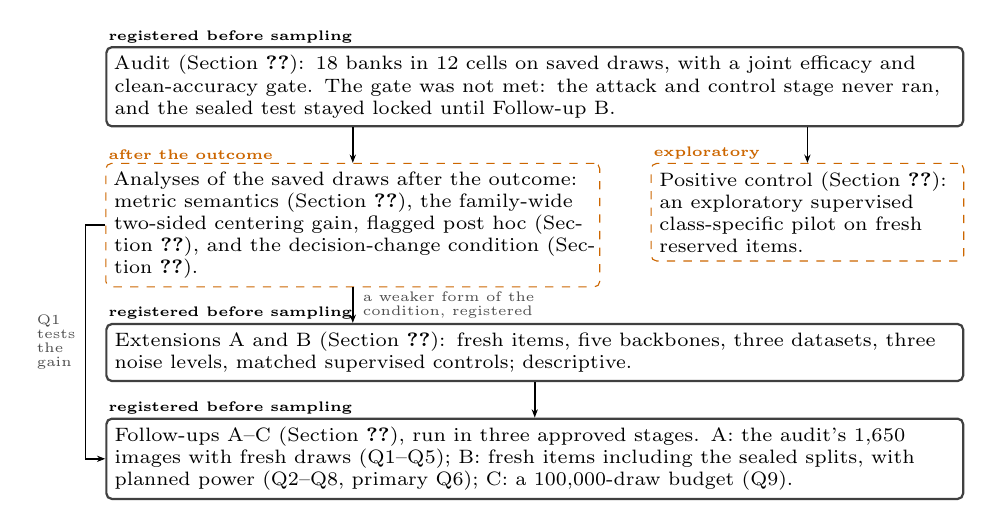
\begin{tikzpicture}[
  font=\scriptsize,
  reg/.style={draw=black!75, thick, rounded corners=2pt, align=left, inner sep=3pt, fill=white},
  post/.style={reg, draw=orange!80!black, dashed, thin},
  arr/.style={-{Stealth[length=3pt]}, semithick},
  tag/.style={font=\tiny\bfseries, anchor=south west, inner sep=1pt},
  lab/.style={font=\tiny, text=black!70, align=left},
]
\node[reg, text width=0.88\columnwidth] (audit) at (0,0) {Audit (Section~\ref{sec:results}):
  \ExpCandidates{} banks in \ExpCells{} cells on saved draws, with a joint efficacy and clean-accuracy
  gate. The gate was not met: the attack and control stage never ran, and the sealed test
  stayed locked until Follow-up B.};
\node[post, text width=0.5\columnwidth, below=4.5mm of audit.south west, anchor=north west] (posthoc)
  {Analyses of the saved draws after the outcome: metric semantics (Section~\ref{sec:semantics}), the
  family-wide two-sided centering gain, flagged post hoc (Section~\ref{sec:grclip}), and the
  decision-change condition (Section~\ref{sec:flip}).};
\node[post, text width=0.31\columnwidth, below=4.5mm of audit.south east, anchor=north east] (control)
  {Positive control (Section~\ref{sec:control}): an exploratory supervised class-specific pilot on
  fresh reserved items.};
\node[reg, text width=0.88\columnwidth, below=4.5mm of posthoc.south west, anchor=north west] (ext)
  {Extensions A and B (Section~\ref{sec:extension}): fresh items, five backbones, three datasets, three
  noise levels, matched supervised controls; descriptive.};
\node[reg, text width=0.88\columnwidth, below=4.5mm of ext.south west, anchor=north west] (fu)
  {Follow-ups A--C (Section~\ref{sec:followup}), run in three approved stages.
  A: the audit's \FUImagesA{} images with fresh draws (Q1--Q5); B: fresh items including the sealed
  splits, with planned power (Q2--Q8, primary Q6); C: a \FUBudgetDraws{}-draw budget (Q9).};
\draw[arr] (audit.south -| posthoc.north) -- (posthoc.north);
\draw[arr] (audit.south -| control.north) -- (control.north);
\draw[arr] (posthoc.south) -- (posthoc.south |- ext.north) node[lab, midway, right] {a weaker form of the\\[-1pt] condition, registered};
\draw[arr] (ext.south) -- (fu.north);
\draw[arr] (posthoc.west) -- ++(-2.5mm,0) |- (fu.west) node[lab, pos=0.25, left] {Q1\\[-1pt]tests\\[-1pt]the\\[-1pt]gain};
\node[tag] at (audit.north west) {registered before sampling};
\node[tag, text=orange!80!black] at (posthoc.north west) {after the outcome};
\node[tag, text=orange!80!black] at (control.north west) {exploratory};
\node[tag] at (ext.north west) {registered before sampling};
\node[tag] at (fu.north west) {registered before sampling};
\end{tikzpicture}
\caption{The studies and what builds on what. Solid boxes were registered,
with their analysis, before any outcome was sampled; dashed boxes followed an
outcome or are exploratory, and are labeled so wherever used. An arrow means
that the later study builds on the earlier one, not the order of execution.}
\label{fig:flow}
\end{figure}


\paragraph{Findings}
\emph{Main result.} In the follow-up, registered before its sampling with
\FUImagesB{} fresh images per noise level, the registered magnitude test
places every primary shared contrast within the $\pm\FUSESOI$-point margin of
no correction at both noise levels under the registered item-pooled mixture of
three datasets, and no interval reaches a gain above $\FUQSixMaxUpper$ points.
This is not confined to collapsed cells: on CIFAR-100 at
$\sigma=\FUSigmaLow$, where the smoothed classifier is not collapsed, two-sided
centering changes certified accuracy by $\FUGRCifarLowPoint$ points. Supervised
class-specific controls, diagnostics rather than matched comparators, gain
$\FUQFiveClassLo$ to $\FUQFiveClassHi$ points (Section~\ref{sec:followup}). In
the descriptive registered extension (five backbones, three datasets, three
noise levels) the largest macro increase among the 17 shared banks was
$\ExtBMaxGridDelta$ points.

\emph{The one exception is setting-dependent.} In the preregistered audit the
registered family did not establish an improvement under the joint efficacy
and clean-accuracy rule. Post hoc, a
GR-CLIP-style two-sided centering, the only operator that also recenters the
image feature, raised standard certified accuracy at radius 0.25 by
$\GRStdDelta$ points (simultaneous 95\% band $[\GRStdLower,\GRStdUpper]$,
conditional on the saved draws); it was excluded because one
\ExpEurosatItemsPerCell-image cell lost \GRWorstCellImages{} images. The
follow-up reproduces this gain under fresh noise on the audit's items; on
fresh items it is not uniform: at $\sigma=\FUSigmaHigh$ it recurs,
descriptively, on sealed EuroSAT for the audit's OpenAI backbones and reverses
on Imagenette and for the LAION-2B-trained OpenCLIP ViT-B/32.

\emph{Mechanism.} For a common text-side translation followed by
per-prototype renormalization, Proposition~\ref{prop:identity} shows that
relative scores can change only through class-dependent renormalization, and
Proposition~\ref{prop:flip} gives a necessary condition for a noisy vote to
change. For the projected-gap translation of Chowers et
al.~\cite{chowers2026bug} all renormalization factors are equal, so
Corollary~\ref{cor:chowers} gives exact decision invariance under hard-label
smoothing. We derived it after the
audit; a weaker form, registered before the extension's sampling, held on fresh
noise with \NthreeCPone{} exceptions.

\emph{Stability is not correctness.} Standard and anchored certified accuracy
differ by \StdAnchGapMin{} to \StdAnchGapMax{} points across candidates at radius 0.25, and
under the uncorrected model \CertifiedWrongRate\% of the audit's positions carry
a certificate for a wrong class at radius 0.25, more than are certified
correct.

\paragraph{Scope}
The audit covers OpenAI CLIP ViT-B/32 and ViT-L/14, CIFAR-100 and
EuroSAT, three folds, Gaussian noise with $\sigma=\ExpSigma$ in the
$224\times224$ model-input space, and shared prototype corrections under a
frozen clean-accuracy eligibility gate. This regime is hard: the
uncorrected smoothed classifier is often collapsed, with smoothed accuracy
between \RangeSmoothedLo\% and \RangeSmoothedHi\% across cells. The extension and
the follow-up add a regime where it is not (CIFAR-100 at $\sigma=\FUSigmaLow$;
Imagenette is near ceiling); EuroSAT remains difficult at every noise level. The audit is not
an equivalence study, it identifies no causal mechanism, and it says nothing
about class-specific, prompt-learned, noise-adapted or image-side methods beyond
the positive control.

\section{Background and Definitions}
\label{sec:background}

\paragraph{Zero-shot prototype classifier}
Let $\phi$ be a frozen CLIP image encoder that maps a model input
$x\in\mathbb R^{3\times224\times224}$ to a unit feature $z=\phi(x)\in\mathbb
S^{d-1}$ (clean inputs lie in $[0,1]^{3\times224\times224}$; noisy inputs are
not clipped),
and let $t_1,\dots,t_K\in\mathbb S^{d-1}$ be unit text prototypes obtained by
encoding one or more prompts per class and renormalizing their mean. The base
classifier is $f(x)=\argmax_k\,\langle\phi(x),t_k\rangle$. A prototype
\emph{operator} replaces the bank $\{t_k\}$ by $\{t'_k\}$ and, for two-sided
operators, also transforms $z$; the base classifier changes accordingly. We
write $\mu_I$ for the mean image feature over a development split and $\mu_T$
for the mean of the $K$ prototypes, and call $\mu_T-\mu_I$ the global modality
gap.

\paragraph{Adversary and noise coordinates}
The adversary is white-box and perturbs the model-input tensor $x$ in
$\ell_2$ norm; it does not control the Gaussian noise draws, the prompts, or
the prototype bank. Noise is added to the $224\times224$ RGB tensor after
deterministic bicubic resizing and center cropping and before channel
standardization, and samples are not clipped. All radii in this paper are
$\ell_2$ distances in that model-input space: a radius of $r=0.25$ over
$3\times224\times224$ coordinates is a root-mean-square per-coordinate change
of $\ExpRadiusPerCoordinate$, below one 8-bit intensity level. Because the
CIFAR and EuroSAT images are upsampled from $32\times32$ and $64\times64$
pixels, these radii are not native-resolution radii and are not comparable to
certificates reported on native CIFAR pixels; Figure~\ref{fig:noise}
(Appendix~\ref{app:followup}) shows one image per dataset at each noise level.
A conservative native-resolution
bound through the operator norm of the resize map is possible but we do not
claim one, because the resize acts on quantized images.

\paragraph{Cohen certification}
For $\varepsilon\sim\mathcal N(0,\sigma^2 I)$ the smoothed classifier is
$g(x)=\argmax_c \Pr[f(x+\varepsilon)=c]$~\cite{cohen2019smoothing}. The
\textsc{Certify} procedure draws $n_0$ noise samples to select a class
$\hat c$ (the first maximum of the selection counts, so an exact tie goes to
the lowest class index), then draws $n$ independent samples to count votes
$k$ for $\hat c$
and forms the one-sided Clopper--Pearson lower confidence bound $p_L$ at
confidence level $1-\alpha$~\cite{clopper1934}. It abstains if $p_L\le\tfrac12$ and otherwise
certifies radius $R=\sigma\,\Phi^{-1}(p_L)$: every $x'$ with
$\lVert x'-x\rVert_2<R$ satisfies $g(x')=\hat c$ with probability at least
$1-\alpha$ over the sampling. This paper uses $n_0=\ExpSelDraws$,
$n=\ExpConfDraws$, $\alpha=\ExpAlpha$, and $\sigma=\ExpSigma$ throughout the
immutable audit. The confidence statement is pointwise: it holds per input, not
simultaneously over a dataset.

\paragraph{Outcome definitions}
Fix a target radius $r$ and a labeled input $(x,y)$ with raw clean prediction
$y_0=f(x)$. Standard Cohen certified accuracy counts the input when the
procedure does not abstain, the selected class equals the label, and the radius
reaches the target:
\begin{equation}
\CA(r)=\Pr\big[\text{no abstain},\;\hat c=y,\;R\ge r\big].
\label{eq:stdca}
\end{equation}
The preregistered audit instead governed selection with a stricter operational
metric that additionally requires the certified class to equal the candidate's
own raw clean prediction:
\begin{equation}
\aCA(r)=\Pr\big[\text{no abstain},\;\hat c=y,\;\hat c=y_0,\;R\ge r\big].
\label{eq:anchca}
\end{equation}
We call \eqref{eq:anchca} anchored certified accuracy. It is a
predicted-label-preservation outcome, not the standard definition, and the two
are reported separately everywhere. The audit used the anchored quantity for its
registered selection rule; standard Cohen certified accuracy is the primary
scientific estimand in the analyses reported here. In \eqref{eq:stdca}, \eqref{eq:anchca} and
below, $\Pr[\cdot]$ is a rate over the evaluated inputs. We also report smoothed accuracy
$\Pr[\hat c=y]$ (the selected class is correct, whether or not the procedure
abstains), the abstention rate, the raw/smoothed agreement rate
$\Pr[\hat c=y_0]$, and the certified-wrong rate
$\Pr[\text{no abstain},\;\hat c\ne y,\;R\ge r]$, the fraction of inputs whose
certificate protects an incorrect class.

\paragraph{Aggregation}
A \emph{cell} is one model--dataset--fold combination. Unless stated otherwise,
a macro value is the unweighted mean over the \ExpCells{} cells, which was the
preregistered estimand. Because CIFAR-100 cells contain
\ExpCifarItemsPerCell{} items and EuroSAT cells \ExpEurosatItemsPerCell{}, we
also report item-pooled values where the weighting matters, and we say which
weighting a number uses.

\section{What a Shared Prototype Operator Can Do to a Noisy Vote}
\label{sec:operators}

% Pipeline schematic (D-146): where the adversary, the noise and each registered operator family act. No data.
\begin{figure*}[t]
\centering
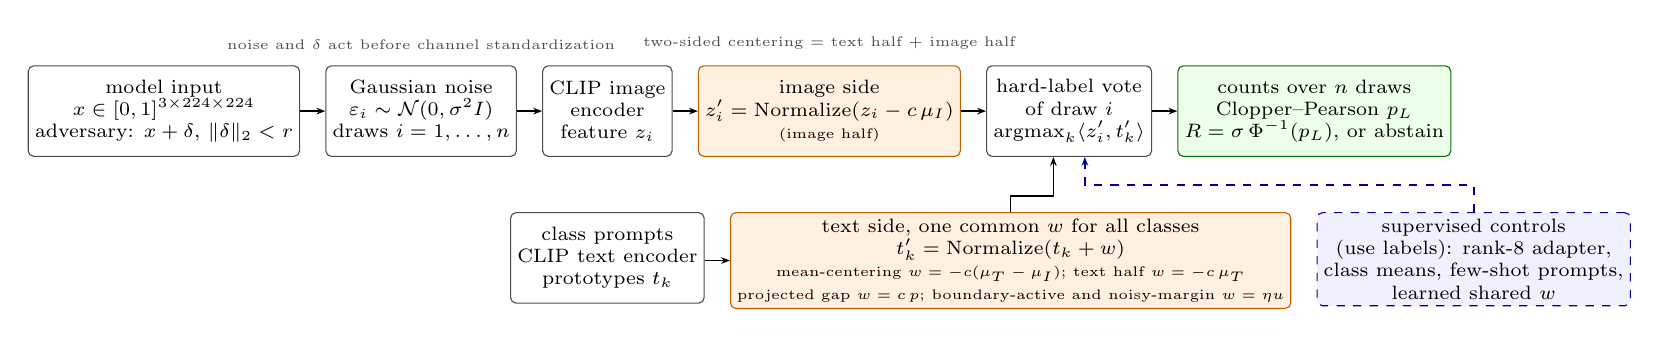
\begin{tikzpicture}[
  font=\scriptsize,
  box/.style={draw=black!70, rounded corners=2pt, align=center, inner sep=2.4pt, minimum height=11.5mm, fill=white},
  op/.style={box, fill=orange!12, draw=orange!75!black},
  sup/.style={box, fill=blue!6, draw=blue!60!black, dashed},
  cert/.style={box, fill=green!8, draw=green!45!black},
  arr/.style={-{Stealth[length=3.2pt]}, semithick},
  note/.style={align=center, font=\tiny, text=black!70},
  node distance=3.2mm,
]
% row 1: the certified path of one input
\node[box] (in) {model input\\ $x\in[0,1]^{3\times224\times224}$\\ adversary: $x+\delta$, $\lVert\delta\rVert_2<r$};
\node[box, right=of in] (noise) {Gaussian noise\\ $\varepsilon_i\sim\mathcal N(0,\sigma^2 I)$\\ draws $i=1,\dots,n$};
\node[box, right=of noise] (enc) {CLIP image\\ encoder\\ feature $z_i$};
\node[op, right=of enc] (imgop) {image side\\ $z'_i=\Normalize(z_i-c\,\mu_I)$\\ {\tiny (image half)}};
\node[box, right=of imgop] (vote) {hard-label vote\\ of draw $i$\\ $\argmax_k\langle z'_i,t'_k\rangle$};
\node[cert, right=of vote] (cert) {counts over $n$ draws\\ Clopper--Pearson $p_L$\\ $R=\sigma\,\Phi^{-1}(p_L)$, or abstain};
\foreach \a/\b in {in/noise, noise/enc, enc/imgop, imgop/vote, vote/cert} {\draw[arr] (\a) -- (\b);}
% row 2: prototypes and the operators that replace them
\coordinate (row2) at ($(in.south)+(0,-7mm)$);
\node[box, anchor=north] (txt) at (row2 -| enc) {class prompts\\ CLIP text encoder\\ prototypes $t_k$};
\node[op, anchor=north west, right=of txt.north east, anchor=north west] (textop) {text side, one common $w$ for all classes\\
  $t'_k=\Normalize(t_k+w)$\\
  {\tiny mean-centering $w=-c(\mu_T-\mu_I)$; text half $w=-c\,\mu_T$}\\
  {\tiny projected gap $w=c\,p$; boundary-active and noisy-margin $w=\eta u$}};
\node[sup, anchor=north west, right=of textop.north east, anchor=north west] (sup) {supervised controls\\ (use labels): rank-8 adapter,\\ class means, few-shot prompts,\\ learned shared $w$};
\draw[arr] (txt.east |- textop.west) -- (textop.west);
\draw[arr] (textop.north) -- ++(0,2mm) -| ($(vote.south)+(-2mm,0)$);
\draw[arr, dashed, blue!60!black] (sup.north) -- ++(0,3.4mm) -| ($(vote.south)+(2mm,0)$);
\node[note, above=0.8mm of noise] {noise and $\delta$ act before channel standardization};
\node[note, above=0.8mm of imgop] {two-sided centering = text half + image half};
\end{tikzpicture}
\caption{Where each registered operator acts. The adversary's perturbation
$\delta$ and the Gaussian noise live in the $224\times224$ model-input space.
Every shared text-side operator translates all prototypes by one common vector $w$
before renormalization, so by Proposition~\ref{prop:flip} it can change a
draw's vote only through the renormalization factors; image-side centering
changes the feature itself. The supervised controls (dashed) use labels; the
class-specific ones bound what is recoverable outside the shared family.}
\label{fig:pipeline}
\end{figure*}


\subsection{The registered operator family}
\label{sec:family}

All operators are fixed per cell from development data only and then frozen;
Figure~\ref{fig:pipeline} shows where each acts. With $\Normalize(v)=v/\lVert
v\rVert$, a coefficient $c\in\{0.25,0.5,1\}$ or a step
$\eta\in\{0.0025,0.005,0.01,0.02,0.04\}$, they are:
\begin{itemize}
\item \emph{Text mean-centering}: $t'_k=\Normalize\big(t_k-c\,(\mu_T-\mu_I)\big)$.
\item \emph{Projected-gap translation} (Chowers et al.~\cite{chowers2026bug}):
$t'_k=\Normalize(t_k+c\,p)$, where $p=(I-VV^{\top})(\mu_I-\mu_T)$ is the
component of $\mu_I-\mu_T$ orthogonal to all differences $t_i-t_j$
($V$ an orthonormal basis of their span).
\item \emph{GR-CLIP-style two-sided centering}: $t'_k=\Normalize(t_k-c\,\mu_T)$
together with $z'=\Normalize(z-c\,\mu_I)$ for every clean or noisy image
feature; the audit used $c=1$, and the follow-up also evaluates its text half
(prototypes only) and its image half ($z$ only).
\item \emph{Clean boundary-active translation}: $t'_k=\Normalize(t_k+\eta u)$
with a unit direction $u$ that increases the normalized clean margin of the
development items' own raw predictions.
\item \emph{Noisy-margin translation}: the same form with a unit direction fitted
to increase a soft noisy-margin objective over Gaussian draws of the development
items at the audit noise level.
\end{itemize}
Together with the identity this gives the \ExpCandidates{} registered banks per
cell. Ground-truth labels are never used to build a direction; the two proposal
directions target each item's own raw clean prediction.

\subsection{Per-draw identity and a decision-change condition}
\label{sec:flip}

Every text-side operator above has the form $t'_k=(t_k+w)/n_k$ with one common
translation $w$ and per-prototype renormalization factors
$n_k=\lVert t_k+w\rVert$. We derived
them after the audit outcome was known, so they explain the audit in hindsight
rather than predicting it; a weaker form of Proposition~\ref{prop:flip} was
registered as a conformance prediction for the extension of
Section~\ref{sec:extension} before its sampling.

% sections/theory_decision_change.tex
% Input from sections/operators.tex inside the subsection labeled sec:flip; no sectioning command here.
% Environments proposition/corollary/remark and the macros \Normalize, \argmax are defined in main.tex.
% Full proofs: sections/appendix_proofs.tex (the Proofs appendix, label app:proofs).
% Derivations, exact code references and the numerical tests behind every statement:
% research/DECISION_CHANGE_CONDITION.md. No result value is typed in this file.

Throughout, $z\in\mathbb S^{d-1}$ is one image feature (the clean feature or
one normalized noisy draw), $s_k=\langle z,t_k\rangle$ are its original scores,
$\omega=\langle z,w\rangle$, and every $n_k$ is positive.

\begin{proposition}[Per-draw identity]
\label{prop:identity}
For every $z$, $\langle z,t'_k\rangle=(s_k+\omega)/n_k$. Hence for every pair
$(j,k)$
\begin{align}
\langle z,t'_j\rangle-\langle z,t'_k\rangle
&=\frac{n_k(s_j+\omega)-n_j(s_k+\omega)}{n_j\,n_k},
\label{eq:identity}\\
n_j-n_k&=\frac{2\,\langle t_j-t_k,\,w\rangle}{n_j+n_k}.
\label{eq:normalizer}
\end{align}
\end{proposition}
\noindent\emph{Sketch.} Expand $\langle z,t_k+w\rangle$, and
$n_j^2-n_k^2=\lVert t_j+w\rVert^2-\lVert t_k+w\rVert^2=2\langle t_j-t_k,w\rangle$
because $\lVert t_j\rVert=\lVert t_k\rVert=1$.

\begin{proposition}[Necessary condition for a decision change]
\label{prop:flip}
Let $s_j\ge s_k$ and suppose that after the translation
$\langle z,t'_k\rangle\ge\langle z,t'_j\rangle$. Then
\begin{align}
0\le s_j-s_k
&\le (n_j-n_k)\,\langle z,t'_j\rangle
\le\lvert n_j-n_k\rvert
\nonumber\\
&=\frac{2\,\lvert\langle t_j-t_k,w\rangle\rvert}{n_j+n_k}
\le\min\{1,\lVert w\rVert\}\,\lVert t_j-t_k\rVert .
\label{eq:flip}
\end{align}
Consequently, for $\lVert w\rVert=\eta$ any pair whose order changes has
original cosine margin at most $\eta\lVert t_j-t_k\rVert\le 2\eta$, and if
the top-1 label of $z$ changes from $j$ to $k$, then the original top-1 margin
of $z$ (winner minus runner-up) is at most
$\lvert n_j-n_k\rvert\le\max_{i,l}\lvert n_i-n_l\rvert$.
\end{proposition}
\noindent\emph{Sketch.} Rearranging the hypothesis with
\eqref{eq:identity}--\eqref{eq:normalizer} gives the first two inequalities,
$\lvert\langle z,t'_j\rangle\rvert\le1$ gives the third, and the last one is
Ptolemy's inequality for the points $t_j$, $t_k$, $-w$, $0$ together with the
reverse triangle inequality (Appendix~\ref{app:proofs}). The second inequality
also carries a direction: when $\langle z,t'_j\rangle>0$ and $s_j>s_k$, the original winner
can lose only to a class whose translated raw norm is strictly smaller,
$n_k<n_j$.

\begin{corollary}[Projected-gap translation is decision-invariant]
\label{cor:chowers}
If $\langle w,t_i-t_j\rangle=0$ for all $i,j$, as for the projected-gap
translation $w=c\,p$ at every coefficient $c$, then all $n_k$ equal one value
$n$ and $\langle z,t'_k\rangle=(s_k+\omega)/n$ with $n$ and $\omega$ independent of $k$,
so the $\argmax$ (including ties) is unchanged for every $z$. In exact
arithmetic with a fixed tie rule, on any fixed set of noisy draws the operator
therefore reproduces the uncorrected hard labels,
vote counts, selected classes, certified radii, and accuracies exactly: it is
an exact invariance control, not a competing method.\footnote{This is the
mechanism behind the identical aggregates of the three projected-gap
coefficients and of the uncorrected bank in the saved audit record; in
floating-point arithmetic only numerical ties could differ.}
\end{corollary}
\noindent\emph{Sketch.} $n_k^2=1+2\langle t_k,w\rangle+\lVert w\rVert^2$ and
$\langle t_k,w\rangle=\langle t_1,w\rangle$ for every $k$.

\begin{corollary}[Finite flip budget]
\label{cor:budget}
Fix $N$ draws $z_1,\dots,z_N$, let $v_i$ be the number of draws whose original
$\argmax$ is $i$, let $k_0=\max_i v_i$, and let $E_F$ be the number of draws
whose original winner $j$ has a competitor $k\ne j$ with
$s_j-s_k\le\lvert n_j-n_k\rvert$; $E_F$ is at most the number of draws whose
original top-1 margin is at most $\max_{i,l}\lvert n_i-n_l\rvert$. After the
translation the counts $v'_i$ satisfy $v'_i\le v_i+E_F$ for every $i$, hence
$\max_i v'_i\le k_0+E_F$. In particular, if $k_0+E_F<k_{\min}$ for a
confirmation threshold $k_{\min}$, then no class reaches $k_{\min}$ on these
draws after the translation.
\end{corollary}
\noindent\emph{Sketch.} By Proposition~\ref{prop:flip} every flipped draw is
one of the $E_F$ eligible draws, and a class gains at most one vote per flipped
draw. Because $E_F$ depends only on the original scores and on the normalizers
$n_k$ recorded when a bank is built, the corollary can rule out a threshold
crossing on these draws, without rescoring, whenever $k_0+E_F<k_{\min}$; when
the inequality fails, it does not show that a crossing occurs. Saved top-1
margins give a looser upper bound on $E_F$, and the exact pairwise count needs
the original score differences. The certificate itself is still computed only
from the hard-label counts by the separate Cohen procedure; the bound is not a
certificate.

\begin{remark}[Two-sided operators]
\label{rem:twosided}
The GR-CLIP-style operator also maps $z\mapsto z'=\Normalize(z-\mu_I)$; we write the
audit's coefficient $c=1$, and a general $c$ replaces $\mu_I$ and $\mu_T$ by $c\mu_I$ and $c\mu_T$.
Renormalizing $z$ never changes an $\argmax$, but the shift does. Assume
$z\neq\mu_I$ and $t_k\neq\mu_T$ for every class $k$, so that both
normalizations are defined. With $n_k=\lVert t_k-\mu_T\rVert>0$,
\begin{align}
\langle z',t'_k\rangle
&=\frac{\langle z-\mu_I,\,t_k-\mu_T\rangle}{\lVert z-\mu_I\rVert\,n_k}
\nonumber\\
&\propto
\frac{s_k-\langle z,\mu_T\rangle-\langle\mu_I,t_k\rangle+\langle\mu_I,\mu_T\rangle}{n_k},
\label{eq:twosided}
\end{align}
where the proportionality constant is common to all classes. The
class-dependent term $-\langle\mu_I,t_k\rangle$ is a per-class bias that no
common text translation produces, so
Propositions~\ref{prop:identity}--\ref{prop:flip} do not bound this operator:
it can change the label of a draw whose original margin exceeds every bound in
\eqref{eq:flip}. This is why, within the audit's registered family, it is the only operator
that can act where the text-only translations cannot.
\end{remark}

\begin{remark}[Engine boundary]
Nothing in this section is a certificate; certified radii are computed
separately from hard-label counts as in Section~\ref{sec:background}.
\end{remark}


Two consequences matter for reading the results. A step of $\eta=0.0025$ can
flip a noisy draw only if its original top-1 margin is at most
$\lvert n_j-n_k\rvert\le2\eta$. The bound defines which draws are eligible;
how many are eligible depends on the empirical margin distribution, and on the
saved draws the registered steps changed very few certified outcomes
(Section~\ref{sec:nearidentity}). The projected-gap
translation leaves every hard label unchanged for every coefficient, so under
hard-label smoothing it is an exact negative control rather than a competing
method; this is a property of the projection Chowers et al.\ designed to
preserve nearest neighbors, made explicit for the smoothed classifier. Within
the audit's registered family, only the two-sided operator, which also shifts
the image feature, escapes the bound.

\subsection{Why a clean global-gap summary cannot settle the question}
\label{sec:nonident}

One might hope to predict a certificate from the clean geometry alone. It cannot
be done in general. Appendix~\ref{app:nonident} gives an explicit smooth
normalized encoder and two binary prototype banks that share the encoder, the
clean feature of the certified input, the complete global-gap vector under any
common image-reference distribution, the clean margin and the prototype
correlation, yet have population Cohen radii that differ by an arbitrary factor.
The two banks are mirror images of one another, and the only asymmetry is how
the encoder's response direction meets each decision boundary; the listed clean
summaries do not contain that response. This is a scoping remark, not a theorem about
CLIP: it motivates measuring noisy votes rather than clean gaps.

\section{Preregistered Audit Design}
\label{sec:design}

\paragraph{Models, data and roles}
The audit, registered in a development stage and a validation stage whose
results were then frozen, uses OpenAI CLIP ViT-B/32 and ViT-L/14 with frozen weights and
frozen prompts: the single OpenAI CIFAR-100 prompt and a three-template EuroSAT
ensemble~\cite{radford2021clip,krizhevsky2009cifar,helber2019eurosat}. From the
CIFAR-100 training split and the EuroSAT image folder we drew three folds, each
with five development and five validation images per class, giving
\ExpCifarItemsPerCell{} validation items per CIFAR-100 cell and
\ExpEurosatItemsPerCell{} per EuroSAT cell, \ExpCells{} cells and
\ExpPositions{} validation positions in total. Development items served only to
build operators, and validation items to select and evaluate them. The
CIFAR-100 test split and a EuroSAT holdout were sealed and were not read by the
audit, the positive control or the extension, whose CIFAR-10 items also come
from the training split; the
registered follow-up of Section~\ref{sec:followup} later spent the sealed
EuroSAT holdout (\FUItemsEurosatB{} items) and \FUItemsCifarB{} CIFAR-100
official-test items once, as its registration specifies.

\paragraph{Certification}
Every candidate bank in every cell was certified on every validation item with
independent selection and confirmation noise streams derived from separate base
seeds, so all \ExpCandidates{} banks of a cell see identical draws (a paired
design), while selection draws are never reused for confirmation. In total the
audit evaluated \ExpRows{} candidate--item positions with \ExpSelVotes{}
selection votes and \ExpConfVotes{} confirmation votes. Radii are reported at
$r\in\{0,0.1,0.25,0.5\}$ with $r=0.25$ preregistered as primary.

\paragraph{Selection and efficacy rule}
The protocol selected one proposal objective and step by the macro
\emph{anchored} certified accuracy at $r=0.25$ over the \ExpCells{} cells, with
frozen tie-breaks, and selected one coefficient per tunable baseline by the same
metric. A candidate was eligible only if its macro clean-accuracy drop relative
to the uncorrected model was at most one point and no single cell dropped by
more than two points. The efficacy gate then required the selected proposal to
exceed the eligible mean-centering comparator on the macro metric and on every
model and dataset marginal. If the gate failed, the protocol stopped: the
preregistered attack and control stage and the sealed test remained
locked, and the project committed to reporting the negative in full. That
stage never ran; the sealed test was later allocated, by a registration hashed
before sampling, to the follow-up
(Section~\ref{sec:followup}).

\paragraph{Custody}
Configurations, split assignments, seeds, prompts and every bank were hashed
before sampling; the reconstruction checks are in
Appendix~\ref{app:deviations}.

\paragraph{Post-hoc audits of the immutable result}
Three analyses were specified after the outcome was known and are labeled as
such. (i) \emph{Metric semantics}: standard certified accuracy
\eqref{eq:stdca} was reconstructed beside the anchored metric \eqref{eq:anchca}
for all candidates, cells and radii. (ii) \emph{Complete-family bands}: a paired
item bootstrap, stratified by dataset, fold and class, resampled the same items
across both models, all candidates, radii and metrics, and produced one
unstudentized 95\% simultaneous max-absolute-deviation band over all
\BandContrasts{} candidate--radius--metric contrasts against the uncorrected
model (\BandReplicates{} replicates, \BandStrata{} strata, seed fixed before
execution). The band is a conditional compatibility statement about the saved
sample; it is not an equivalence test. (iii) \emph{Exact-count adjudication}:
the clean gate was recomputed with integer counts because the implementation
compared floating-point percentages.

\section{Audit Results}
\label{sec:results}

% Complete-family contrast figure at radius 0.25. Data generated by
% scripts/generate_satml2027_figure_data.py from immutable artifacts.
\begin{figure}[t]
\centering
% Generated by scripts/generate_satml2027_figure_data.py; do not edit.
\pgfplotsset{familyaxis/.style={
  ytick={1,2,3,4,5,6,7,8,9,10,11,12,13,14,15,16,17},
  yticklabels={{Mean-centering c=0.25},{Mean-centering c=0.5},{Mean-centering c=1},{Projected gap c=0.25},{Projected gap c=0.5},{Projected gap c=1},{Two-sided centering c=1},{Boundary-active 0.0025},{Boundary-active 0.005},{Boundary-active 0.01},{Boundary-active 0.02},{Boundary-active 0.04},{Noisy-margin 0.0025},{Noisy-margin 0.005},{Noisy-margin 0.01},{Noisy-margin 0.02},{Noisy-margin 0.04}}}}

\begin{tikzpicture}
\begin{axis}[
  width=0.9\columnwidth,
  height=0.72\columnwidth,
  xlabel={Change in certified accuracy at $r=0.25$ vs.\ no correction (points)},
  ylabel={},
  y dir=reverse,
  ymin=0.5, ymax=17.5,
  familyaxis,
  yticklabel style={font=\tiny},
  xticklabel style={font=\tiny},
  xlabel style={font=\scriptsize},
  legend style={font=\tiny, at={(0.02,0.02)}, anchor=south west, draw=none, fill=white, fill opacity=0.85},
  grid=major,
  grid style={gray!25},
  every axis plot/.append style={mark size=1.4pt},
]
\draw[gray!60, dashed] (axis cs:0,0.5) -- (axis cs:0,17.5);
\addplot+[only marks, mark=*, color=black, error bars/.cd, x dir=both, x explicit, error mark options={rotate=90, mark size=1.2pt}]
  table[x=std_delta, y=y, x error=std_err] {generated/fig_family_r025.dat};
\addlegendentry{Standard Cohen CA}
\addplot+[only marks, mark=o, color=blue!70!black, error bars/.cd, x dir=both, x explicit, error mark options={rotate=90, mark size=1.2pt}]
  table[x=anch_delta, y expr=\thisrow{y}+0.3, x error=anch_err] {generated/fig_family_r025.dat};
\addlegendentry{Anchored CA}
\end{axis}
\end{tikzpicture}
\caption{Change in certified accuracy against the identity (no correction) for
each of the \ExpOperatorBanks{} other registered banks, at the primary radius,
under both metrics. Bars are the common 95\% simultaneous
max-absolute-deviation band over all \BandContrasts{} contrasts. At this
radius only the two-sided centering operator's band excludes zero; the
projected-gap banks are exactly zero; the proposal banks change at most
\ChangedPositionsProposalsMax{} of the \ExpPositions{} certified outcomes.}
\label{fig:family}
\end{figure}


\subsection{The preregistered gate failed}
\label{sec:gate}

Figure~\ref{fig:family} and Table~\ref{tab:family} (Appendix~\ref{app:tables})
report every registered bank at the primary radius under both metrics with its
post-hoc simultaneous band. The saved selection was
the clean boundary-active bank at step 0.0025, with anchored certified accuracy
\SavedAnchCA\% against \NoCorrAnchCA\% for no correction, and standard
certified accuracy \SavedStdCA\% against \NoCorrStdCA\%. No mean-centering
coefficient passed the clean gate, so the protocol's fallback comparator was
the projected-gap bank at coefficient 0.5, which is identical to no correction
in every decision in exact arithmetic (Corollary~\ref{cor:chowers}); the saved proposal exceeded it
by one position in anchored certified accuracy, the protocol's selection metric,
while its standard certified accuracy was lower. The efficacy rule also required strictly positive margins
against mean-centering on every model and dataset marginal; computed for the
exact-count proposal against each of the three mean-centering coefficients,
all \ForcedComparisonFailures{} of these forced contrasts failed on at least one
marginal, one only by a single position. The negative decision is therefore a failure
to establish efficacy under the frozen joint rule. It is not evidence that the
effect is zero.

\paragraph{Exact-count adjudication}
The implementation compared percentage differences in floating point, so a
one-image drop in a \ExpEurosatItemsPerCell-image cell was represented as
$\FloatGateArtifact$ rather than $2.0$ and was rejected. Recomputing the written
rule with integer counts makes \FloatGateRejectedCandidates{} further banks
eligible and changes the selected proposal to step 0.04 (standard
\ExactStdCA\%, anchored \ExactAnchCA\%). The gate decision does not change under
either reading; the saved selection is preserved and both readings are reported.

\subsection{The proposal banks were near-identity operators}
\label{sec:nearidentity}

Proposition~\ref{prop:flip} gives a necessary condition for vote changes, which
the follow-up finds loose (Section~\ref{sec:followup}); the proposals were also
small. The saved proposal
moved the prototype bank by a macro Frobenius displacement of \DispSaved{},
against \DispGMCOne{} for text mean-centering at coefficient one and \DispGR{}
for two-sided centering; the largest step reaches \DispExact{}. On the saved
draws, the six proposal banks with steps up to 0.01 change the standard
certified outcome at $r=0.25$ of at most \ChangedPositionsSmallSteps{} of the
\ExpPositions{} positions, the boundary-active step-0.04 bank changes
\ChangedPositionsExactStep{}, and the two-sided operator changes
\ChangedPositionsGR{}. The three projected-gap banks give the same certified
outcomes and reported aggregates as the uncorrected model, as
Corollary~\ref{cor:chowers} predicts in exact arithmetic; a few saved
confirmation counts differ slightly, consistent with floating-point numerical
ties (on fresh draws the follow-up bounds every such change by a registered
tie budget, Q4 in Section~\ref{sec:followup}), and their largest absolute contrast is
\ChowersMaxAbsDelta{} points. The registered family thus contained \ExpDistinctClassifiers{} distinct
classifiers, of which the text-only proposals changed very few saved certified
outcomes and the largest text-only translations damaged clean accuracy.

The common band, a single-step resampling band in the sense of Westfall and
Young~\cite{westfall1993resampling}, has a half-width of \BandHalfWidth{}
points set by the noisiest contrasts (the large-displacement comparators at
small radii), many times the paired standard error of the proposal contrasts;
it is uninformative about the proposals, and the counts above describe them.

\subsection{One shared operator did move certified correctness}
\label{sec:grclip}

In this post-hoc complete-family analysis, whose bands are simultaneous and
conditional on the saved draws, the GR-CLIP-style two-sided centering is, at the
primary radius, the only bank whose simultaneous interval excludes zero under
either metric: $\GRStdDelta$ points of standard certified accuracy at
$r=0.25$ with band $[\GRStdLower,\GRStdUpper]$, and $\GRAnchDelta$ points
anchored with band $[\GRAnchLower,\GRAnchUpper]$. Across the whole family,
\BandExclZero{} contrasts exclude zero: \BandExclZeroGR{} of the eight
contrasts of this operator, all positive, and \BandExclZeroOther{} negative
standard-metric contrasts of text mean-centering at $r=0$
(Section~\ref{sec:semantics}). It is therefore the only bank with a positive
interval that excludes zero. Its macro clean accuracy rose to \GRClean\% from \NoCorrClean\%, and
clean accuracy improved in \GRCellsImproved{} of \ExpCells{} cells. It was
ineligible because one cell (\GRWorstCell) lost \GRWorstCellDrop{} points, that
is \GRWorstCellImages{} of \ExpEurosatItemsPerCell{} images.

Three qualifications bound the size of this effect without removing it. The
gain is $\GRStdDeltaCifar$ points on the six CIFAR-100 cells, where
\GRStdCifarCellsNegative{} of six cells move down, and $\GRStdDeltaEurosat$
points on the six \ExpEurosatItemsPerCell-image EuroSAT cells; the band that
excludes zero is carried by the EuroSAT cells (Appendix~\ref{app:tables}).
Second, every bootstrap stratum contains five items, and resampling five items
with replacement understates the variance by a factor of $4/5$; inflating the
band accordingly gives $[\GRStdLowerSens,\GRStdUpperSens]$, which still
excludes zero. Third, the preregistered estimand weights the \ExpCells{} cells
equally, so the EuroSAT cells carry half the estimand (Kish design effect
\KishDesignEffect{}, effective sample size \EffectiveN{}); the item-pooled gain
is $\GRStdDeltaPooled$ points. The operator is also the only one in the audit's registered family that
transforms the image feature, which is exactly the case that
Proposition~\ref{prop:flip} does not bound. We do not conclude that two-sided
centering is effective in general: within the audit, the registered clean gate
rather than the certificate excluded it, and the follow-up finds it in its
original setting, while on fresh items it lies within the $\pm\FUSESOI$-point
margin under the pooled estimand and changes sign across datasets and
checkpoints (Section~\ref{sec:followup}).

\subsection{Stability is not correctness}
\label{sec:semantics}

For every candidate, at $r=0.25$ anchored certified accuracy lies \StdAnchGapMin{} to
\StdAnchGapMax{} points below standard certified accuracy, because the anchored
metric additionally discards positions whose stable class is correct but
differs from the raw clean prediction: for the uncorrected model,
\CertifiedCorrectAnchorMismatch{} of the \PartCertifiedCorrect{}
certified-correct positions at $r=0.25$ are such anchor mismatches. The two
metrics can also disagree. Text mean-centering at
coefficient one has a standard contrast of $\GMCStdDeltaRZero$ points at $r=0$
with band $[\GMCStdLowerRZero,\GMCStdUpperRZero]$, which excludes zero, while
its anchored contrast at the same radius is $\GMCAnchDeltaRZero$ points with
band $[\GMCAnchLowerRZero,\GMCAnchUpperRZero]$; it raises raw/smoothed
agreement to \GMCAgreement\% from \NoCorrAgreement\% while lowering clean
accuracy to \GMCClean\%. An evaluation that reports only one of the two metrics
can therefore reach a different conclusion about the same operator.

% Generated by scripts/generate_satml2027_paper_assets.py; do not edit by hand.
% Failure partition at radius 0.25 (no correction and GR-CLIP).
% Sources (SHA-256):
%   results/EXP-20260906-017/cells/openai-clip-vit-b32-quickgelu__cifar100__fold0/cohen_sufficient_statistics.pt  6a92e1fa347b69bf86177d8c83f1b56d86fa44cac18973888534ccfdcbe4ed24
%   results/EXP-20260906-017/cells/openai-clip-vit-b32-quickgelu__cifar100__fold1/cohen_sufficient_statistics.pt  b93944f38e875849b3c6bd7f801da17437cef4f6bc01e08fb170f24afde6c741
%   results/EXP-20260906-017/cells/openai-clip-vit-b32-quickgelu__cifar100__fold2/cohen_sufficient_statistics.pt  6a3ec93e8c02bba40951201fe4db41ee4de606f64e90dc3d5cad11408eaf566e
%   results/EXP-20260906-017/cells/openai-clip-vit-b32-quickgelu__eurosat__fold0/cohen_sufficient_statistics.pt  72209d45477462c72d81581621fc78d45905c0cf04a8f6f2af5de72e9b714be8
%   results/EXP-20260906-017/cells/openai-clip-vit-b32-quickgelu__eurosat__fold1/cohen_sufficient_statistics.pt  3b7041dcf554efa8cf0b0bf1d04939171871c44cb09c14f77fc434a0b35db802
%   results/EXP-20260906-017/cells/openai-clip-vit-b32-quickgelu__eurosat__fold2/cohen_sufficient_statistics.pt  c777fdc36b84e306d4a35df39394a19f978e928c778626c11ba4a46d0d5e5adf
%   results/EXP-20260906-017/cells/openai-clip-vit-l14-quickgelu__cifar100__fold0/cohen_sufficient_statistics.pt  78370b2e707dd1978d5c6af28ada0b6a1f00026997ada5065d68c5040d5d8e8e
%   results/EXP-20260906-017/cells/openai-clip-vit-l14-quickgelu__cifar100__fold1/cohen_sufficient_statistics.pt  b16b30871366d8eb30d671fb2b4637448686d2651b84da57166c35d128e20e3c
%   results/EXP-20260906-017/cells/openai-clip-vit-l14-quickgelu__cifar100__fold2/cohen_sufficient_statistics.pt  fb526b42b45fa8f5c056e6617a17531fe7a2b6b0e8b4de8c71d4dec48ebe4e2e
%   results/EXP-20260906-017/cells/openai-clip-vit-l14-quickgelu__eurosat__fold0/cohen_sufficient_statistics.pt  e30909c6244b8e85ccb18ea41a084ef606aad7c93dbaae8ee46b17a3987fcb98
%   results/EXP-20260906-017/cells/openai-clip-vit-l14-quickgelu__eurosat__fold1/cohen_sufficient_statistics.pt  97ac1ff7f79cc60e6bb4e11375d45f15abbb196bd42a4a635fff7e344af02def
%   results/EXP-20260906-017/cells/openai-clip-vit-l14-quickgelu__eurosat__fold2/cohen_sufficient_statistics.pt  9bd16331a58fd0801251624d2fe4d5ea6e037d8a413ea8478887b1b268cbb106
%   artifacts/negative_paper/exp017_scientific_soundness_audit_v1.json  1e8676e0a999c4bba2130106bdfe786dc082f803573929ce5701be48928349b0
\begin{table}[t]
\centering
\scriptsize
\setlength{\tabcolsep}{3pt}
\caption{Failure partition at radius 0.25 pooled over 3,300 positions for no correction and the GR-CLIP-style two-sided candidate, under the standard metric and the anchored metric. Counts come from the audit's saved per-example sufficient statistics and reproduce its per-cell failure categories.}
\label{tab:partition}
\begin{tabular}{lrrrr}
\toprule
Outcome at $r=0.25$ & No corr.\ $n$ & \% & GR-CLIP $n$ & \% \\
\midrule
\multicolumn{5}{l}{\emph{Standard metric}} \\
Abstained & 821 & 24.88 & 815 & 24.70 \\
Nonabstaining, wrong smoothed class & 1,677 & 50.82 & 1,681 & 50.94 \\
\quad of which certified wrong at 0.25 & 706 & 21.39 & 719 & 21.79 \\
Correct smoothed class, radius $<0.25$ & 303 & 9.18 & 271 & 8.21 \\
Certified correct at 0.25 & 499 & 15.12 & 533 & 16.15 \\
\midrule
\multicolumn{5}{l}{\emph{Anchored metric}} \\
Abstained & 821 & 24.88 & 815 & 24.70 \\
Nonabstaining anchor mismatch & 1,688 & 51.15 & 1,635 & 49.55 \\
Anchor preserved, raw class wrong & 103 & 3.12 & 112 & 3.39 \\
Anchor correct, radius $<0.25$ & 255 & 7.73 & 246 & 7.45 \\
Anchored certified correct at 0.25 & 433 & 13.12 & 492 & 14.91 \\
\bottomrule
\end{tabular}
\end{table}


Table~\ref{tab:partition} partitions the \ExpPositions{} positions of the
uncorrected model at $r=0.25$ (item-pooled). Abstentions account for
\PartAbstain{} positions; \PartWrongClass{} nonabstaining positions select a
class other than the label, and \PartCertifiedWrong{} of them carry a
certificate at this radius; \PartCorrectBelowRadius{} select the correct class
but do not reach the radius; and \PartCertifiedCorrect{} are certified correct.
Under the anchored metric, \PartAnchorMismatch{} nonabstaining positions are
anchor mismatches and \PartAnchoredCorrect{} remain anchored and certified
correct. Wrong smoothed classes are the dominant loss, and the certified-wrong
rate, \CertifiedWrongRate\% of all positions, exceeds the certified-correct
rate. Within a cell, the single most frequent class among certified-wrong
positions accounts for \CWTopClassShareLo\% to \CWTopClassShareHi\% of them.
Across cells, raw clean accuracy ranges from \RangeCleanLo\% to
\RangeCleanHi\%, smoothed accuracy from \RangeSmoothedLo\% to
\RangeSmoothedHi\%, raw/smoothed agreement from \RangeAgreementLo\% to
\RangeAgreementHi\%, the share of positions with zero radius under the anchored
metric from \RangeZeroRadiusLo\% to \RangeZeroRadiusHi\%, and the largest
single smoothed-class share from \RangeTopClassLo\% to \RangeTopClassHi\%.
These are descriptions of where certificates are lost in this regime,
consistent with the high-noise degradation reported by~\cite{nirala2024ovc};
the controlled experiments that would identify a cause were never run, and we
make no causal claim.

\paragraph{Finite confirmation budget}
Every estimate here concerns the finite-budget procedure. With
\ExpConfDraws{} confirmation draws, fewer than the $10^5$ of Cohen et
al.~\cite{cohen2019smoothing}, the exact bound censors radii: at $r=0.25$,
\CensoredNoCorrRQuarter{} uncorrected positions and \CensoredSavedRQuarter{}
for the saved proposal. Pairing does not equalize this censoring; Q9 measures
a larger confirmation budget directly (Section~\ref{sec:followup}).

\section{Positive Control: Is Certified Correctness Recoverable at All?}
\label{sec:control}

A negative result for shared operators says little unless some intervention
can move the certificate in the same regime. We therefore report a separate, exploratory, supervised
\FarlaShots-shot class-specific pilot, originally developed as a candidate class-specific method and
used here only as a positive control, on fresh reserved items of the same two
backbones, datasets and noise level, with \FarlaCifarConfirmItems{} CIFAR-100
and \FarlaEurosatConfirmItems{} EuroSAT confirmation items per cell and the same
certification budget. Using \FarlaShots{} labeled images per class, it trained
class-specific low-rank tangent adjustments of the prototype bank in the spirit
of parameter-efficient adaptation~\cite{hu2022lora} under a noisy-and-clean
cross-entropy objective. Seven variants were evaluated (Table~\ref{tab:farla}):
a supervised \emph{shared} translation (one common correction, the
comparator); a \emph{low-rank} adapter with the cross-entropy objective only; a
\emph{tail-only} variant that adds a loss on the vote fraction near the
certification threshold; the \emph{full} objective at rank 8, at rank 4, and in
a direct (non-tangent) parametrization; and a \emph{pseudo-label} variant of the
full objective trained on the model's own clean predictions instead of labels.
The pilot was registered with its own configuration and
custody package, but its planned smoke run was skipped, so we call it
exploratory.

% Generated by scripts/generate_satml2027_paper_assets.py; do not edit by hand.
% Positive-control pilot candidates and planned contrasts.
% Sources (SHA-256):
%   FARLA/downloaded_results/EXP-20260917-020-FARLA-FULL/analysis/report.json  dd123e618475ebb498583fb569e26040f45cf051b6d8338224d61af37a2777c4
%   FARLA/downloaded_results/EXP-20260917-020-FARLA-FULL/config_snapshot.json  57b79923fd333c01fb128e7dc88f81f9aefce7e6b3aafff4d373d5c5d5511620
%   FARLA/downloaded_results/EXP-20260917-020-FARLA-FULL/splits/manifest.json  cdda5225e1220b207d084a57a23c6771e396c0ba5dda57d3f7223710097d960d
\begin{table*}[t]
\centering
\scriptsize
\setlength{\tabcolsep}{4pt}
\caption{Positive-control pilot: macro standard CA, anchored CA and certified-wrong rate at radius 0.25 and macro clean accuracy over 4 cells (1,000 CIFAR-100 and 100 EuroSAT confirmation items per cell, 20 supervised shots per class), with all five planned paired contrasts and their class-stratified percentile bootstrap 95\% intervals (10,000 replicates). Clean gate: macro drop at most 1 point and every cell drop at most 2 points.}
\label{tab:farla}
\begin{tabular}{lrrrrc}
\toprule
Candidate & Std CA & Anch.\ CA & Clean & Cert.-wrong & Clean gate \\
\midrule
No correction & 11.60 & 8.43 & 60.88 & 34.18 & pass \\
Shared translation (noisy CE) & 11.75 & 8.68 & 61.28 & 33.43 & pass \\
Low-rank r=8 (noisy CE) & 27.10 & 23.35 & 72.50 & 13.58 & pass \\
Tail-only r=8 & 36.50 & 28.75 & 70.80 & 9.05 & pass \\
Full objective r=4 & 33.35 & 24.60 & 62.15 & 11.78 & pass \\
Full objective r=8 & 35.05 & 29.55 & 68.58 & 10.43 & pass \\
Full objective, direct & 34.60 & 31.20 & 66.23 & 11.43 & fail \\
Full objective r=8, pseudo-labels (no ground truth) & 27.10 & 21.15 & 46.98 & 17.75 & fail \\
\bottomrule
\end{tabular}
\par\vspace{4pt}
\begin{tabular}{lrrr}
\toprule
Planned contrast (Std CA) & $\Delta$ & 95\% lower & 95\% upper \\
\midrule
Full objective r=8 vs.\ no correction & $+23.45$ & $+20.25$ & $+26.63$ \\
Full objective r=8 vs.\ tail-only r=8 & $-1.45$ & $-4.05$ & $+1.13$ \\
Full objective r=8 vs.\ full objective r=4 & $+1.70$ & $-0.65$ & $+4.00$ \\
Full objective r=8 vs.\ low-rank r=8 (noisy CE) & $+7.95$ & $+4.73$ & $+11.15$ \\
Low-rank r=8 (noisy CE) vs.\ shared translation (noisy CE) & $+15.35$ & $+12.70$ & $+18.03$ \\
\bottomrule
\end{tabular}
\end{table*}


Table~\ref{tab:farla} shows that class-specific adaptation recovers a large
share of certified correctness in a regime where shared translations did not:
standard certified accuracy at $r=0.25$ rises from \FarlaIdentityStdCA\% to
\FarlaFullStdCA\% for the full rank-8 variant, a paired macro gain of
$\FarlaVsNoCorrDelta$ points with 95\% interval
$[\FarlaVsNoCorrLower,\FarlaVsNoCorrUpper]$, while the supervised shared
translation reaches only \FarlaSharedStdCA\%. The certified-wrong rate falls
from \FarlaIdentityCW\% to \FarlaFullCW\%. Four qualifications bound the
reading. The tail-only ablation reaches \FarlaTailStdCA\%, above the full variant's
point estimate, with a certified-wrong rate of \FarlaTailCW\%, and the full
variant's contrast against it is
$\FarlaVsTailDelta$ points with interval
$[\FarlaVsTailLower,\FarlaVsTailUpper]$; that interval does not establish a
difference, so the additional certificate-aware terms are not shown to be
necessary. Clean accuracy also rises, from
\FarlaIdentityClean\% to \FarlaFullClean\% (and to \FarlaTailClean\% for the
tail-only variant), so these results do not isolate a benefit specific to
certificate targeting from ordinary accuracy improvement under supervised
adaptation. The pseudo-label variant, the only one that uses no
ground truth, reaches \FarlaPseudoStdCA\% standard certified accuracy
($\FarlaPseudoVsNoCorrDelta$ points,
$[\FarlaPseudoVsNoCorrLower,\FarlaPseudoVsNoCorrUpper]$) but lowers clean
accuracy to \FarlaPseudoClean\%, a drop of \FarlaPseudoCleanDrop{} points that
fails the clean gate: it buys certified stability at the cost of clean
correctness, which is the trade this paper argues must be reported explicitly.
Finally, the pilot itself was not compared with noise-aware prompt
learning~\cite{hussein2024promptsmooth}, the natural baseline for any text-side
adaptation; the follow-up adds a few-shot prompt control inspired by it
(Section~\ref{sec:followup}). The control therefore establishes a scope boundary: the certificate
in this regime is movable by class-specific supervised adaptation, and the
result of Section~\ref{sec:results} concerns shared operators only.

\section{Registered Extension: Five Backbones, Three Datasets, Three Noise Levels}
\label{sec:extension}

After the audit, we registered a separate extension with hashed
configurations (Table~\ref{tab:extension}, Appendix~\ref{app:tables}) before
sampling any of its evaluation outcomes, to probe the scope of the earlier
findings; every registered cell completed and is reported regardless of sign.
It re-estimates the same
\ExpCandidates{} banks on a fresh development split, adds four prospectively
trained supervised controls with \FarlaShots{} labels per class (a learned
shared translation in two forms, a noisy class-mean bank, and a
rank-8 class-specific tangent adapter), and evaluates all \ExtBanks{} banks on
fresh items in two registered experiments: Extension A, the two audit backbones at $\sigma\in\{0.12,0.5\}$ on CIFAR-100,
EuroSAT and CIFAR-10 (\ExtPrimaryCellsA{} primary cells plus two CIFAR-10
bridge cells at $\sigma=0.25$), and Extension B, OpenAI ViT-B/16, OpenAI RN50 and an
OpenCLIP ViT-B/32 trained on LAION-2B~\cite{schuhmann2022laion5b,cherti2023openclip} at
$\sigma\in\{0.25,0.5\}$ (\ExtCellsB{} cells), with \ExtItemsCifar{} items per
CIFAR cell and \ExtItemsEurosat{} per EuroSAT cell and the same
\ExtUniqueItems{} unique items reused across cells. The registered primary
outcome per experiment is the equal-cell macro change in standard certified
accuracy at $r=\sigma$ against no correction, with one shared-item
class-stratified simultaneous band over the 21 contrasts.

\paragraph{Regime}
Table~\ref{tab:ext-regime} (Appendix~\ref{app:tables}) reports the uncorrected
model in every cell. At
$\sigma=0.12$ the CIFAR cells are far from collapsed: smoothed accuracy ranges
from \ExtSmoothedTwelveCifarLo\% to \ExtSmoothedTwelveCifarHi\% and standard
certified accuracy at $r=\sigma$ from \ExtStdCATwelveCifarLo\% to
\ExtStdCATwelveCifarHi\%, while the EuroSAT cells remain difficult
(\ExtSmoothedTwelveEurosatLo\% to \ExtSmoothedTwelveEurosatHi\% smoothed).
At $\sigma=0.5$ every dataset collapses. The extension therefore contains the
non-degenerate regime that the immutable audit lacked.

\paragraph{Outcomes}
Table~\ref{tab:ext-contrasts} (Appendix~\ref{app:tables}) lists every
registered contrast. In the audit
backbones (Extension A) the largest increase among the 17 banks of the shared
grid is $\ExtAMaxGridDelta$ points (\ExtAMaxGridId{}) and the smallest change is
$\ExtAMinGridDelta$ points (\ExtAMinGridId{}, with clean accuracy
$\ExtAMinGridCleanDelta$ points); at a common half-width of \ExtACritical{}
points, \ExtAGridExclZero{} of the 17 grid bands excludes zero
(\ExtAGridExclZeroIds{}). Two-sided
centering changes standard certified accuracy by $\ExtAGRDelta$ points
($[\ExtAGRLower,\ExtAGRUpper]$) and clean accuracy by $\ExtAGRCleanDelta$
points. In the three further backbones (Extension B) the largest increase in the
shared grid is $\ExtBMaxGridDelta$ points (\ExtBMaxGridId{}), the smallest
$\ExtBMinGridDelta$ (\ExtBMinGridId{}), \ExtBGridExclZero{} of 17 grid
bands exclude zero with half-width \ExtBCritical{} points, and two-sided
centering changes standard certified accuracy by $\ExtBGRDelta$ points
($[\ExtBGRLower,\ExtBGRUpper]$). Against the registered
$\pm\ExtRegionPoints$-point reporting region (prediction X1; the registrations
number their predictions X1 and X3 to X5), \ExtAInsideRegion{} and
\ExtBInsideRegion{} of the 17 grid changes lie inside it
(Table~\ref{tab:ext-contrasts}). In the two CIFAR-10 bridge cells at the
audit's noise level two-sided centering changes certified accuracy by
$\ExtBridgeGRDeltaBthirtytwo$ points (ViT-B/32) and
$\ExtBridgeGRDeltaLfourteen$ points (ViT-L/14).

The supervised controls behave differently. The learned shared translation,
which like the shared family applies one common vector to every prototype
(its tangent form rescales each prototype by a factor fixed by that vector;
Appendix~\ref{app:proofs}) but is fitted with labels, changes certified
accuracy by $\ExtASharedTangentDelta$ points
($[\ExtASharedTangentLower,\ExtASharedTangentUpper]$) in Extension A and
$\ExtBSharedTangentDelta$ points in Extension B, so prediction X3 (the shared
control stays inside the band), scored as registered on the tangent form, was
\ExtXthreeSummary{}; the pure form, which reuses its vector, changes it by $\ExtASharedPureDelta$
($[\ExtASharedPureLower,\ExtASharedPureUpper]$) and $\ExtBSharedPureDelta$
points ($[\ExtBSharedPureLower,\ExtBSharedPureUpper]$). The
class-specific rank-8 adapter changes certified accuracy by
$\ExtALowrankDelta$ points ($[\ExtALowrankLower,\ExtALowrankUpper]$, clean
$\ExtALowrankCleanDelta$ points) and $\ExtBLowrankDelta$ points
($[\ExtBLowrankLower,\ExtBLowrankUpper]$), and the noisy class-mean bank,
which replaces text prototypes by image-side class means, by
$\ExtANoisyMeanDelta$ points while changing clean accuracy by
$\ExtANoisyMeanCleanDelta$ points; prediction X4 (at least one per-class
control leaves the band upward) was \ExtXfourSummary{}, and \ExtXfourFlags{}.
Prediction X5 (the identity bank's
top-class share and predicted-class Gini rise with $\sigma$ in every model and
dataset) was \ExtXfiveSummary{}: in Extension B the share fell between
$\sigma=0.25$ and $\sigma=0.5$ in several RN50 and ViT-B/16 cells; we report the
decline without an explanation.

\paragraph{Reading}
On fresh items, across five backbones and three noise levels, including cells
where the smoothed classifier is not collapsed, the largest macro increase in
the 17-bank shared grid was $\ExtAMaxGridDelta$ points (audit backbones) and
$\ExtBMaxGridDelta$ points (further backbones), and the separately trained
shared tangent control changed the macro by
$\ExtASharedTangentDelta$ and $\ExtBSharedTangentDelta$ points, with bands
containing zero in both experiments. The largest grid decrease in Extension A,
$\ExtAMinGridDelta$ points, came from the largest text-side translation, which
also lost clean accuracy; in Extension B that translation changed certified
accuracy by $\ExtBGMCOneDelta$ points and clean accuracy by
$\ExtBGMCOneCleanDelta$ points. Class-specific
capacity fitted with the same supervision moved certified accuracy by
$\ExtALowrankDelta$ and $\ExtBLowrankDelta$ points. The extension is descriptive:
its cell sizes of \ExtItemsCifar{} and \ExtItemsEurosat{} items were fixed
without a registered power calculation, the power of any contrast depends on
the paired discordance and on the dependence between repeated items, its bands
are conditional on the realized draws, and no equivalence is claimed.
Execution deviations and verification status are in
Appendix~\ref{app:deviations}.

\paragraph{Fresh-noise mechanism diagnostic}
The four-cell diagnostic at $\sigma=0.25$ records per-draw features so that
the flip condition can be checked directly. Its registered conformance
prediction (every draw whose label changes under a shared translation
satisfies the inequality of Proposition~\ref{prop:flip}) recorded
\NthreeCPone{} exceptions; the descriptive flip-budget partition and the
useful/harmful taxonomy are in Table~\ref{tab:n3c} (Appendix~\ref{app:tables}).

% Prospective follow-up (EXP-021), brought into the paper by D-145. Every number is a macro from
% generated/macros.tex (design: the three registrations; results: the registered analysis outputs).

\section{Prospective Follow-Up: Fresh Noise, Fresh Items, Larger Budget}
\label{sec:followup}

After the extension we registered a three-part follow-up
(Table~\ref{tab:followup-design}) before sampling any
of its outcomes, to answer the questions the audit left open. Follow-up A
re-certifies the audit's \FUImagesA{} images with the
audit's saved bank tensors, fresh certification draws and a fresh pipeline; it
is a same-item re-certification, not an independent replication. Follow-up B
uses fresh, never-used items: \FUBackbonesB{} backbones (the two
audit backbones and an OpenCLIP ViT-B/32 trained on
LAION-2B~\cite{schuhmann2022laion5b,cherti2023openclip}), CIFAR-100 test
(\FUItemsCifarB{} items), sealed EuroSAT (\FUItemsEurosatB{}) and Imagenette,
a ten-class ImageNet subset~\cite{howard2019imagenette} (\FUItemsImagenetteB{}), at
$\sigma\in\{\FUSigmaLow,\FUSigmaHigh\}$. Its registered planning calculation
(Table~\ref{tab:followup-design}; not the operating power of the bootstrap)
gives the pooled family at each $\sigma$ (\FUImagesB{} unique images) a minimum
detectable effect of \FUPooledMDE{} points and the EuroSAT family alone \FUEurosatMDE{}. Its primary
estimand is item-pooled, whereas the audit's was equal-cell; both are reported.
Follow-up C re-certifies \FUItemsC{} items per dataset with \FUBudgetDraws{}
confirmation draws to test the \FUConfDraws{}-draw budget. Every cell of
Follow-ups A and B evaluates the same \FUBanks{} banks (Follow-up C, three of them):
the identity; text mean-centering, the projected-gap translation, two-sided
centering and its text-only and image-only halves at \FUCoefficients{}
coefficients each; both proposal objectives at \FUSteps{} steps up
to \FUStepMax{}; and \FUControls{} supervised controls. Inference uses a
class-stratified shared-item bootstrap with \FUReplicates{} replicates,
Holm-adjusted direction tests, and practical-magnitude classes against a
smallest effect of interest of \FUSESOI{} points, fixed with the planning
calculation before sampling; the margin is a registered convention, not a
claim that smaller changes are unimportant.

The registered questions are: whether the post-hoc two-sided gain persists
under fresh draws (Q1); how much of it the text and image halves carry (Q2);
whether text-side steps change only draws that Proposition~\ref{prop:flip}
allows, and whether the projected-gap bank is decision-invariant draw by draw
(Q3, Q4); what the supervised controls achieve (Q5); whether any shared
operator changes standard certified accuracy on fresh items, and by at least
\FUSESOI{} points (Q6, primary); whether the result persists where the
smoothed classifier is not collapsed (Q7); whether the radii are comparable to
the literature (Q8); and how many certificates change with the larger budget
(Q9). Every question is reported below or in Appendix~\ref{app:followup},
whatever its outcome. The registered analysis ran once, unchanged, after a
recorded analysis-stage approval; cells not run: \FUNotRunA{} of \FUCellsA{} in
Follow-up A and \FUNotRunB{} of \FUCellsB{} in Follow-up B
(Appendix~\ref{app:deviations}).

% Results (D-145). Outcome-neutral text written before the analysis ran: every number, verdict and bank name is a
% macro from the registered analysis outputs (analysis/exp021/021{a,b,c}); only the Reading paragraph interprets.
% EXP-021B registered contrasts at both noise levels (D-146). Rows fixed before any outcome existed. Data:
% generated/fig_followup_forest_{primary,shared,supervised}.dat, written by scripts/generate_satml2027_paper_assets.py
% from the pooled families of analysis/exp021/021b/analysis_ext.json; a framed placeholder until that output exists.
\begin{figure}[t]
\centering
% Generated by scripts/generate_satml2027_paper_assets.py; do not edit by hand.
\def\FUForestReady{1}
\def\FUForestXmin{-8.38}
\def\FUForestXmax{11.49}
\def\FUForestRows{11}
\pgfplotsset{fuforestaxis/.style={xmin=-8.38, xmax=11.49, ytick={1,2,3,4,5,6,7,8,9,10,11}, yticklabels={{Two-sided centering $c{=}1$},{\quad its text half},{\quad its image half},{Boundary-active step 0.16},{Noisy-margin step 0.16},{Text mean-centering $c{=}1$},{Projected gap $c{=}1$},{Learned shared translation},{Rank-8 tangent adapter},{Few-shot prompt bank},{Noisy class-mean bank}}}}
\def\FUForestSeparators{5.5,7.5}

\ifnum\FUForestReady=1
\begin{tikzpicture}
\begin{axis}[
  width=0.78\columnwidth,
  height=0.66\columnwidth,
  fuforestaxis,
  y dir=reverse,
  ymin=0.4, ymax=11.6,
  set layers,
  xlabel={Change in standard certified accuracy at $r=\sigma$ vs.\ no correction (points)},
  yticklabel style={font=\tiny},
  xticklabel style={font=\tiny},
  xlabel style={font=\scriptsize},
  legend style={font=\tiny, at={(0.5,1.02)}, anchor=south, draw=none, legend columns=2,
                /tikz/every even column/.append style={column sep=6pt}},
  legend cell align=left,
  grid=major,
  grid style={gray!25},
  every axis plot/.append style={mark size=1.4pt},
  error bars/error mark options={rotate=90, mark size=1.2pt},
]
\addplot[draw=none, fill=gray!18, on layer=axis background, forget plot]
  coordinates {(-\FUSESOI,0.4) (\FUSESOI,0.4) (\FUSESOI,11.6) (-\FUSESOI,11.6)} \closedcycle;
\addplot[gray!60, dashed, forget plot] coordinates {(0,0.4) (0,11.6)};
\foreach \sep in \FUForestSeparators {
  \edef\temp{\noexpand\addplot[gray!55, forget plot] coordinates {(\FUForestXmin,\sep) (\FUForestXmax,\sep)};}
  \temp
}
% sigma low: filled black; sigma high: open blue, offset 0.3 down; marker shape by group
\pgfplotsset{
  fulo/.style={only marks, black, mark options={fill=black}, error bars/x dir=both, error bars/x explicit},
  fuhi/.style={only marks, blue!70!black, mark options={fill=white}, error bars/x dir=both, error bars/x explicit},
}
\addplot[fulo, mark=*] table[x=lo, y=y, x error minus=lo_minus, x error plus=lo_plus]
  {generated/fig_followup_forest_primary.dat};
\addlegendentry{$\sigma=\FUSigmaLow$}
\addplot[fuhi, mark=o] table[x=hi, y expr=\thisrow{y}+0.3, x error minus=hi_minus, x error plus=hi_plus]
  {generated/fig_followup_forest_primary.dat};
\addlegendentry{$\sigma=\FUSigmaHigh$}
\addplot[fulo, mark=diamond*, forget plot] table[x=lo, y=y, x error minus=lo_minus, x error plus=lo_plus]
  {generated/fig_followup_forest_shared.dat};
\addplot[fuhi, mark=diamond, forget plot] table[x=hi, y expr=\thisrow{y}+0.3, x error minus=hi_minus, x error plus=hi_plus]
  {generated/fig_followup_forest_shared.dat};
\addplot[fulo, mark=square*, forget plot] table[x=lo, y=y, x error minus=lo_minus, x error plus=lo_plus]
  {generated/fig_followup_forest_supervised.dat};
\addplot[fuhi, mark=square, forget plot] table[x=hi, y expr=\thisrow{y}+0.3, x error minus=hi_minus, x error plus=hi_plus]
  {generated/fig_followup_forest_supervised.dat};
\end{axis}
\end{tikzpicture}
\else
\framebox[0.95\columnwidth]{\parbox[c][0.45\columnwidth][c]{0.85\columnwidth}{\centering\scriptsize
  Placeholder: this figure is drawn from the registered Follow-up B analysis output\\
  (the five primary contrasts, two unsupervised reference banks and the four supervised
  controls at both noise levels).}}
\fi
\caption{Registered Follow-up B contrasts on fresh items, pooled over datasets and
backbones: change in standard certified accuracy at $r=\sigma$ against no
correction, with unadjusted 95\% bootstrap intervals, at
$\sigma=\FUSigmaLow$ (filled) and $\sigma=\FUSigmaHigh$ (open). The shaded band
is the registered smallest effect of interest, $\pm\FUSESOI$ points. Circles
are the registered primary family (magnitude classes in
Table~\ref{tab:followup}); diamonds are two unsupervised reference banks;
squares are the supervised controls, which use labels. The rows were fixed
before any outcome existed.}
\label{fig:followup-forest}
\end{figure}


\paragraph{Audit items under fresh draws (Follow-up A)}
Under fresh draws, two-sided centering changes the audit items' equal-cell
macro certified accuracy by $\FUQOnePoint$ points
($[\FUQOneLower,\FUQOneUpper]$), against $\FUQOneSaved$ points on the saved
draws; the registered Q1 verdict is \emph{\FUQOneVerdict}: a positive
direction (\FUQOnePDirection) and no detected shortfall (\FUQOnePShortfall),
which is not a claim of equality. Item-pooled, the change is
$\FUQOnePooledPoint$ points ($[\FUQOnePooledLower,\FUQOnePooledUpper]$)
against $\FUQOnePooledSaved$ (\FUQOnePooledVerdict). In the item-pooled
decomposition (Q2) the text half alone changes certified accuracy by
$\FUQTwoAText$ points, the image half by $\FUQTwoAImage$, and their
interaction is $\FUQTwoAInter$.

\paragraph{Fresh items (Follow-up B, primary)}
Figure~\ref{fig:followup-forest} shows the registered primary family (Q6):
two-sided centering at $c=1$, its text half, its image half, and the two
proposals at step 0.16, each against no correction; Table~\ref{tab:followup}
(Appendix~\ref{app:followup}) gives both estimands and the adjusted classes.
Two-sided centering changes standard certified accuracy at $r=\sigma$ by
$\FUGRLowPoint$ points ($[\FUGRLowLower,\FUGRLowUpper]$) at
$\sigma=\FUSigmaLow$ and by $\FUGRHighPoint$ ($[\FUGRHighLower,\FUGRHighUpper]$)
at $\sigma=\FUSigmaHigh$ (equal-cell $\FUGRLowMacroPoint$ and
$\FUGRHighMacroPoint$); its Holm-adjusted classes are \FUGRClasses{}. At
$\sigma=\FUSigmaLow$ the Holm-adjusted direction is positive for
\FUQSixLowPositiveIds{} and negative for \FUQSixLowNegativeIds{}; at
$\sigma=\FUSigmaHigh$ it is negative for \FUQSixHighNegativeIds{}. Direction
and magnitude answer different questions: a contrast can be resolved in sign
and still lie inside the margin. Descriptively, the unadjusted 95\% intervals of
all ten primary pooled contrasts lie within $\pm\FUQSixMaxAbsBound$ points,
and none reaches a gain above $\FUQSixMaxUpper$ points. Across the \FUQSixLowN{} primary contrasts the magnitude
classes are \FUQSixLowGain{} gain, \FUQSixLowLoss{} loss, \FUQSixLowEquiv{}
practically equivalent and \FUQSixLowIncon{} inconclusive at
$\sigma=\FUSigmaLow$, and \FUQSixHighGain{}, \FUQSixHighLoss{},
\FUQSixHighEquiv{} and \FUQSixHighIncon{} at $\sigma=\FUSigmaHigh$. Among all
unsupervised banks the largest point estimates are $\FUQSixLowMaxPoint$
(\FUQSixLowMaxId) and $\FUQSixHighMaxPoint$ points (\FUQSixHighMaxId), and the
smallest $\FUQSixLowMinPoint$ (\FUQSixLowMinId) and $\FUQSixHighMinPoint$
(\FUQSixHighMinId). The text half alone changes certified accuracy by
$\FUQTwoLowText$ and $\FUQTwoHighText$ points at the two noise levels, the
image half by $\FUQTwoLowImage$ and $\FUQTwoHighImage$, and their interaction
is $\FUQTwoLowInter$ and $\FUQTwoHighInter$ (Q2; every coefficient in
Table~\ref{tab:followup-registered}). The supervised controls (Q5), the regime
of the uncorrected model (Q7), the orientation against published radii (Q8)
and, descriptively, the certified-accuracy curves of four banks fixed in
advance (Figure~\ref{fig:followup-curves}) are in Appendix~\ref{app:followup}.

\paragraph{Draw-level checks and budget}
Q3 (text-side steps change only draws that Proposition~\ref{prop:flip}
allows) \FUQThreeSummary{}. Its coarse form is necessary but loose: on the
audit's items the coarse flip budget admits \FUQThreeBudgetLo\% of draws at step
\FUQThreeStepMin{} and \FUQThreeBudgetFour\% at step 0.04, whereas
\FUQThreeChangedLo\% to \FUQThreeChangedFour\% change, and useful and harmful
changes nearly cancel (\FUQThreeUsefulFour{} against \FUQThreeHarmfulFour{} for
the boundary-active proposal at step 0.04; Table~\ref{tab:followup-steps}).
Q4 (the projected-gap bank is decision-invariant draw by draw)
\FUQFourSummary{}, with \FUQFourChangedA{} (A) and \FUQFourChangedB{} (B) changed
draws, all within the
registered numerical tie budget: no correction's margin between the two
classes involved was at most $\FUQFourMarginA$ and $\FUQFourMarginB$ (the
tolerance plus the largest renormalization difference), a bound that does not
identify the cause of a change. With
\FUBudgetDraws{} instead of \FUConfDraws{} confirmation draws (Q9, Follow-up C),
the uncorrected model's certified-correct count at $r=\sigma$ over its
\FUCellsC{} cells moves from \FUQNineIdFour{} to \FUQNineIdFull{} of
\FUQNineItems{} (\FUQNineIdGained{} gained, \FUQNineIdLost{} lost); over the
\FUBanksC{} registered banks \FUQNineAllChanged{} of \FUQNineAllCerts{}
certificates change, at most \FUQNineMaxChanged{} for \FUQNineMaxId. The two
registered determinism checks, exact identity with Follow-up B of the
confirmation prefix and of the full certificate inputs, returned
\emph{\FUQNinePrefixIdentity} and \emph{\FUQNineInputIdentity}.

% Reading: written after the registered outputs existed (D-152), revised after the review of 2026-09-28 (D-153) to
% report the dataset and backbone heterogeneity; it interprets Q1, Q6, Q5 and Q7 only.
\paragraph{Reading}
Under fresh draws the post-hoc two-sided gain on the audit's items persists
($\FUQOnePoint$ against $\FUQOneSaved$ points), matching its registered
prediction, so it is not specific to the saved certification draws; it is
carried by the image half and, descriptively, by the EuroSAT cells
($\FUQOneEurosat$ against $\FUQOneCifar$ points on CIFAR-100). On fresh items
it does not transport as a uniform gain. Under the registered item-pooled
mixture of the three datasets (weights $3{:}1{:}3$) it lies within the
registered $\pm\FUSESOI$-point margin at both noise levels and, in an unregistered
comparison, below the fresh-draw estimates on the audit's items at
$\sigma=\FUSigmaHigh$ (item-pooled $\FUGRHighPoint$ against
$\FUQOnePooledPoint$ points, equal-cell $\FUGRHighMacroPoint$ against
$\FUQOnePoint$); the sign of this small aggregate even depends on the
weighting. Its dataset and backbone estimates range from positive to negative:
on sealed EuroSAT at that $\sigma$ its direction is positive
($\FUGREurosatHighPoint$ points; descriptively $\FUGREurosatHighOBthirtytwo$ and
$\FUGREurosatHighOLfourteen$ for the two audit backbones but
$\FUGREurosatHighLBthirtytwo$ for the LAION-2B-trained model), and on Imagenette it
is negative ($\FUGRImagenetteHighPoint$). All five registered primary contrasts
are classified as practically equivalent to no correction at both noise
levels, with small resolved effects of both signs, and no unsupervised bank's
pooled estimate exceeds $\FUQSixMaxBoth$ points; the only contrast classified
as a dataset-level gain under its registered within-family procedure,
$\FUQSixDsMaxPoint$ points for \FUQSixDsMaxId{} on \FUQSixDsMaxData{} at
$\sigma=\FUQSixDsMaxSigma$, comes with a clean-accuracy change of
$\FUQSixDsMaxFamilyClean$ points there, and the clean rule flags it. Where the classifier is not collapsed and supervision
moves the certificate, on CIFAR-100 at $\sigma=\FUSigmaLow$ (smoothed accuracy
\FUQSevenCifarLowSmoothedLo\% to \FUQSevenCifarLowSmoothedHi\%), two-sided
centering changes certified accuracy by $\FUGRCifarLowPoint$ points; Imagenette
is near ceiling (at least \FUQSevenImagenetteStdCALo\% certified correct at
$r=\sigma$), and even the supervised controls move it by only
$\FUQFiveClassImagenetteLo$ to $\FUQFiveClassImagenetteHi$ points. The controls
that change the prototypes class by class gain $\FUQFiveClassLo$ to
$\FUQFiveClassHi$ points pooled, mostly on EuroSAT and with clean-accuracy
changes of their own (Appendix~\ref{app:followup}), whereas one label-fitted
shared vector changes certified accuracy by $\FUQFiveLowSharedPoint$ and
$\FUQFiveHighSharedPoint$ under the item-pooled estimand but by
$\FUQFiveSharedEurosatLow$ and $\FUQFiveSharedEurosatHigh$ on EuroSAT. The
follow-up therefore delimits the audit's post-hoc exception rather than
overturning it: the gain persists in its original setting but has no stable,
transportable direction on fresh items, and the pooled result places it
within the registered margin without implying a zero effect in every dataset
or checkpoint.

% Related Work for the SaTML 2027 submission (IEEEtran conference, 10pt).
% Bib keys are restricted to the approved list. No result value is typed here;
% if a number is ever needed it must come from generated/macros.tex.

\section{Related Work}

\paragraph{Randomized smoothing and certified accuracy}
Randomized smoothing certifies an $\ell_2$ radius for the Gaussian-smoothed classifier, which returns the class most probable under input noise \cite{lecuyer2019pixeldp,li2019certified,cohen2019smoothing}. Cohen et al.\ give the radius $\sigma\,\Phi^{-1}(p_L)$ from a lower confidence bound $p_L$ and the \textsc{Certify} procedure, which selects a class from one set of draws and bounds its probability from a second \cite{cohen2019smoothing}. Salman et al.\ train the base classifier against attacks on the smoothed model \cite{salman2019provably}; Yang et al.\ characterize the radii attainable under other norms and noise shapes \cite{yang2020randomized}; Kumar et al.\ certify average class scores and margins \cite{kumar2020certifying}, so the use of confidence or margin information inside smoothing is established. In this literature, certified accuracy counts an input only when the smoothed class equals the label and its radius reaches the target; it does not ask whether the smoothed class agrees with the noise-free prediction of the base model. We keep this estimand and report the raw-clean-anchored variant as a separate operational quantity. That smoothing shrinks decision regions unevenly across classes is known \cite{mohapatra2021hidden}, and abstention-aware certified metrics exist for segmentation \cite{anani2024adaptive}; the certified-wrong rate we report is a reporting recommendation grounded in these observations, not a new metric.

\paragraph{Certified vision-language classification}
Nirala et al.\ certify open-vocabulary CLIP classifiers with randomized smoothing, reuse earlier computation when prompts change, and report that certified accuracy degrades sharply as the noise grows \cite{nirala2024ovc}. Our audit runs in a high-noise regime of the kind they describe, and we do not present that degradation as a finding. Seferis et al.\ certify generative vision-language models by mapping their outputs to an oracle classification task \cite{seferis2025randomized}; we study frozen prototype classifiers. PromptSmooth learns textual prompts \cite{zhou2022coop} under Gaussian noise so that a frozen medical vision-language model certifies better \cite{hussein2024promptsmooth}; it is the direct precedent for any text-side adaptation of a smoothed CLIP classifier, and the shared operators we audit are far more constrained than learned prompts. Carlini et al.\ denoise the input with a diffusion model before a pretrained classifier \cite{carlini2023dds}; this image-side route lies outside our operator family and is not evaluated. In embedding space, Pautov et al.\ smooth normalized embeddings and convert an embedding-boundary distance into an $\ell_2$ radius for prototype classifiers \cite{pautov2022smoothed}, and RetrievalGuard certifies smoothed nearest-neighbor retrieval \cite{wu2022retrievalguard}. Xia et al., in a preprint under review, bound cosine feature deviation by a Gaussian robustness score and convert it into a top-one prototype certificate through the clean margin and prototype correlation \cite{xia2026feature}. None of these feature certificates enters our estimates; every certificate we report is a hard-label Cohen certificate of the smoothed version of its frozen classifier (the supervised controls are not zero-shot).

\paragraph{The modality gap and its corrections}
Liang et al.\ define the modality gap of contrastive encoders such as CLIP \cite{radford2021clip}, attribute it to initialization and contrastive optimization, and show that shifting it changes zero-shot behavior in a task-dependent way \cite{liang2022mind}. Schrodi et al.\ find that a few dimensions drive the gap and that its influence on accuracy is often overshadowed by other factors \cite{schrodi2025twoeffects}, and Fahim et al.\ show that contrastive training separates even samples of one modality \cite{fahim2024contrastive}; Levi and Gilboa show that CLIP's image and text embeddings lie on linearly separable ellipsoid shells not centered at the origin \cite{levi2025double}. That the global gap magnitude does not explain accuracy is therefore established. Post-hoc corrections form the operator families we audit. Text-side mean-centering and the two-sided variant that also recenters image features are normalized zero-shot adaptations of the GR-CLIP calibration \cite{li2025closing}. Chowers et al.\ treat the gap as a robustness feature: under a centered-orthogonality assumption and additive noise in embedding space, translating one modality toward the other provably improves a nearest-neighbor stability measure, and a projected translation preserves clean nearest neighbors \cite{chowers2026bug}. Our audit does not contradict that theorem. It concerns a different object, the hard-label vote of a classifier smoothed with pixel noise, and shows that the normalized zero-shot adaptation of their projected operator cannot change any such vote. Sato et al.\ show that clean gap reduction can change class-relative decisions and induce prediction hubness \cite{sato2026hubness}; the certified-wrong class concentration we report arises without any correction and under Gaussian pixel noise, and must not be read as correction-induced clean hubness. Empirical robustness work aligns image and text representations during robust fine-tuning or by training-free projection \cite{dong2025stabilizing,zhu2025cola,dong2025pathsimplices,dong2025subspaces} or fine-tunes the vision encoder adversarially \cite{schlarmann2024robustclip}. These methods target attack accuracy rather than Cohen certificates and lie outside our frozen shared operator family.

\paragraph{Preregistration and post-selection inference}
Nosek et al.\ argue that preregistration separates hypothesis generation from hypothesis testing \cite{nosek2018preregistration}. Kuchibhotla et al.\ review the bias that arises when the same data select a candidate and estimate its effect, and the simultaneous-inference remedies \cite{kuchibhotla2022postselection}. Our validation split both selected and evaluated candidates, so we report the complete family under one simultaneous band and describe the selected candidate rather than test it. Lakens notes that an equivalence claim needs a prespecified smallest effect of interest and a dedicated procedure \cite{lakens2017equivalence}; the audit registered neither and claims no absence of effect, and the follow-up registered both before its sampling (Section~\ref{sec:followup}).

\paragraph{What is and is not new}
New here are a necessary decision-change condition for a renormalized common text-side translation under hard-label smoothing, stated per draw, with the corollary that the projected-gap operator is decision-invariant; a metric-semantics audit that keeps standard certified accuracy, raw-clean-anchored stability, abstention, and certified-wrong concentration separate and shows that these estimands rank operators differently; and a preregistered audit that reports the complete operator family with simultaneous bands, including the one operator whose band excludes zero at the primary radius, followed by a follow-up, registered with a planning power calculation before its sampling, that delimits that operator's gain on fresh items. Not new, and not claimed, are certified zero-shot or open-vocabulary VLM classifiers and their degradation at high noise \cite{nirala2024ovc}; mean-centering and projected gap corrections \cite{li2025closing,chowers2026bug}; noise-aware prompt adaptation \cite{hussein2024promptsmooth}; finite-sample certification machinery \cite{cohen2019smoothing}; class-specific low-rank adaptation \cite{hu2022lora}, used here only as a supervised positive control; and feature-space or embedding certificates \cite{xia2026feature,pautov2022smoothed}.

% Limitations and lessons for the SaTML 2027 submission.
% Every number in this file is a macro from generated/macros.tex; see
% paper/satml2027/MACROS_CONTRACT.md. No result value is typed by hand.

\section{Limitations and Lessons for Certified-VLM Evaluation}

\subsection{Limitations}

The extension and the follow-up address the audit's main gaps (a non-collapsed
regime, fresh items, a planned sample size); the limitations that remain are these.

\begin{itemize}
\item \textit{Noise regime.} In the audit, Gaussian noise with $\sigma=\ExpSigma$ is added in the model-input space after bicubic upsampling of small native images. Our radii are distances in that model-input space; because the resize acts on quantized images, no exact conversion to native-resolution radii exists, and our radii are not comparable with certificates reported at native resolution. Smoothed accuracy collapses in this regime, as Nirala et al.\ observed for CLIP at larger noise \cite{nirala2024ovc}: without correction it ranges across cells from \RangeSmoothedLo\% to \RangeSmoothedHi\%, and raw/smoothed agreement from \RangeAgreementLo\% to \RangeAgreementHi\%.
\item \textit{Breadth.} The audit covers two OpenAI CLIP backbones, two datasets, frozen prompt templates, and one noise level in \ExpCells{} cells. The registered extension and follow-up add backbones, datasets, and noise levels; the extension's cell sizes were fixed without a registered power calculation, and its cells reuse the same \ExtUniqueItems{} items, so its contrasts are dependent; it is reported descriptively and regardless of sign. In the follow-up, the non-collapsed evidence rests on CIFAR-100 at $\sigma=\FUSigmaLow$: Imagenette is near ceiling, where even the supervised controls barely move the certificate, and the dataset families are secondary. The follow-up spent the sealed EuroSAT holdout, so a later confirmatory study needs new items. Nothing here transfers to other prompts, class-conditioned or prompt-level methods, image-side denoising, native-resolution regimes, or certificates other than hard-label Cohen certificates, such as soft-score or feature-space ones.
\item \textit{Power.} The audit's band (half-width \BandHalfWidth{} points) is uninformative about the proposals, which moved standard certified accuracy by $\SavedStdDelta$ and $\ExactStdDelta$ points; underpowered paired comparisons are common in this field \cite{card2020power}. The band conditions on the realized votes and establishes neither equivalence nor a uniform minimum detectable effect; a finite-stratum correction widens it to \BandHalfWidthSens{} points. Equal-cell weighting has Kish design effect \KishDesignEffect{} (effective sample size \EffectiveN{} of \ExpPositions{} positions), so item-pooled aggregates are reported alongside. The follow-up registered a planning power calculation before sampling; it assumes a paired discordance and is not the operating power of its bootstrap analysis.
\item \textit{Gate design.} The per-cell clean rule's two-point tolerance is one image in a \ExpEurosatItemsPerCell{}-image cell, and it decided the two-sided operator's exclusion. The production gate compared in floating point and rejected exact two-point drops for \FloatGateRejectedCandidates{} candidates (exact-count re-adjudication is reported alongside), and the positive decision path required an eligible mean-centering comparator, none of which existed, so the forced fallback comparison was decided at single-image resolution.
\item \textit{Post-selection.} The validation split both selected candidates and produced the reported outcomes. We therefore report all \ExpCandidates{} registered candidates under one simultaneous band, and describe rather than test the selected candidate. The audit registered no smallest effect of interest, so it makes no equivalence or evidence-of-absence claim \cite{lakens2017equivalence}; the follow-up registered one (\FUSESOI{} points) before sampling, and only its registered magnitude classes use it.
\item \textit{Confirmation budget.} Each position used \ExpConfDraws{} confirmation draws at $\alpha=\ExpAlpha$. At radius $r=\sigma$, \CensoredNoCorrRQuarter{} no-correction positions have a plug-in estimate that would certify the radius but a finite-sample lower bound that does not; at radius zero, \CensoredNoCorrRZero{} positions select the correct class but abstain. In Follow-up C, \FUBudgetDraws{} instead of \FUConfDraws{} draws changed \FUQNineAllChanged{} of \FUQNineAllCerts{} certificates at $r=\sigma$; the selection budget was not varied.
\item \textit{Positive control.} The class-specific low-rank control is supervised with \FarlaShots{} labeled images per class. Its clean accuracy rises from \FarlaIdentityClean\% to \FarlaFullClean\%, so its certified gain is not isolated from ordinary clean-accuracy improvement under supervision, and the full-versus-tail-only interval does not establish a difference ($\FarlaVsTailDelta$ points, interval $\FarlaVsTailLower$ to $\FarlaVsTailUpper$). It bounds what remains recoverable outside the shared family; it does not rescue that family and is not proposed as a method. In the follow-up, a few-shot prompt control inspired by noise-aware prompt learning \cite{hussein2024promptsmooth} gains about as much as its rank-8 adapter.
\item \textit{Causal identification.} Active, inactive, random, and sign-reversed control interventions were never run. Anchor disagreement, certified-wrong concentration, candidate displacement, and vote collapse are descriptive observations, not identified causes.
\item \textit{Certificate confidence.} Each certificate holds with probability at least $1-\alpha$ for its own position. The fraction of certified positions is not a family-wise event, and no simultaneous coverage across positions is claimed.
\item \textit{Verification.} All verification was internal to the author team: other authors re-evaluated or replayed every result, several checks with AI assistance, labeled as such in the review ledger; no party outside the team has reproduced the chain (Appendix~\ref{app:deviations}).
\end{itemize}

\subsection{Lessons}
\label{sec:lessons}

The audit suggests a minimal reporting template for certified vision-language classifiers.
\begin{enumerate}
\item Report standard certified accuracy in the sense of Cohen et al.\ \cite{cohen2019smoothing}, and label any raw-clean-anchored or predicted-label-stability variant as a separate quantity.
\item Report abstention and the certified-wrong rate at every radius, together with the class concentration of certified-wrong predictions.
\item Report raw/smoothed agreement per cell.
\item Report both equal-cell and item-pooled aggregates, with the design effect of the chosen weighting, and per-dataset and per-backbone effects beside pooled ones.
\item State eligibility rules as exact counts, state the per-cell granularity in images, and never compare thresholds in floating point.
\item Report the complete registered family with simultaneous bands, including inert and ineligible members.
\item State the noise coordinate system and the native resolution, and say whether reported radii are comparable across resolutions.
\end{enumerate}

\section{Conclusion}
\label{sec:conclusion}

We audited whether shared corrections of CLIP's prototype geometry improve the
certified correctness of a frozen zero-shot classifier under randomized
smoothing. A per-draw identity shows that a renormalized common text-side
translation can change a hard-label vote only through the difference between
prototype renormalization factors, which makes the projected-gap translation
exactly inert under hard-label smoothing. The preregistered audit did not
establish an improvement under its joint rule; its one post-hoc exception,
two-sided centering, persisted under fresh noise on the audit's items. A
follow-up registered before its sampling delimits that exception: on fresh
items every primary shared contrast lies within the $\pm\FUSESOI$-point margin
under the registered item-pooled estimand, while at $\sigma=\FUSigmaHigh$ the
gain recurs, descriptively, on sealed EuroSAT for the audit's backbones and
reverses on Imagenette and for the LAION-2B-trained model. Supervised
class-specific controls raise certified accuracy, with clean-accuracy changes
of their own; a label-fitted shared vector does not. The evidence marks a
transportability boundary rather than an impossibility: shared corrections can
move certified correctness in particular settings, but not as a consistent
gain across datasets and checkpoints. A certificate supports trust only when an
evaluation also reports whether the stabilized prediction is correct and how
the conclusion varies across data and models
(Section~\ref{sec:lessons}).\label{body:end}%
% body:end marks the last line of the page-limited body (scripts/check_satml2027_submission.py).


% Open Science section for the SaTML 2027 submission. Unnumbered; the
% disclosure order is Open Science, LLM usage considerations, Ethical
% Considerations, references (V5 review 1). Per the call it does not count
% towards the page limit. The anonymous repository link is entered in HotCRP, not here.
% V3-audit correction M5 (2026-09-26): the section states the release boundary
% per claim group; hashes of omitted files identify them but do not make them
% replayable.

\section*{Open Science}

\paragraph{Release boundary}
The anonymous artifact linked from the submission form is assembled from
hash-identified files by the artifact deadline, and its manifest lists every
file with its SHA-256. The table below states, for each group of claims, the
inputs the artifact provides, what those inputs let a reviewer recompute on a
CPU, and what is omitted. A hash identifies an omitted file; it does not make
that file replayable.

\begin{center}
\footnotesize
\begin{tabular}{@{}p{0.19\columnwidth}p{0.47\columnwidth}p{0.24\columnwidth}@{}}
\toprule
\raggedright Claims & \raggedright Released inputs; recomputable on a CPU & \raggedright Omitted, listed by hash\tabularnewline
\midrule
\raggedright Audit metrics, bands and gate (Sec.~\ref{sec:results}) & \raggedright Protocol and registrations; per-example selection and confirmation counts, certified radii and clean predictions for all \ExpCandidates{} candidates in all \ExpCells{} cells; candidate metadata, bank hashes and development tensors; the simultaneous-analysis configuration and output. Recomputes every audit table and macro, the complete-family band and the exact-count gate. & \raggedright None\tabularnewline
\addlinespace
\raggedright Theory (Sec.~\ref{sec:flip}, App.~\ref{app:nonident}--\ref{app:proofs}) & \raggedright Decision-change note, verification scripts and tests, non-identification constructions. Recomputes every numerical check of the propositions. & \raggedright None\tabularnewline
\addlinespace
\raggedright Positive control (Sec.~\ref{sec:control}) & \raggedright Configuration snapshot, split indices, trained adapters, confirmation outputs, analysis report and custody manifest. Recomputes every aggregate and the paired bootstrap. & \raggedright Feature cache (about 0.8\,GB)\tabularnewline
\addlinespace
\raggedright Extension (Sec.~\ref{sec:extension}) & \raggedright Registrations and code; per-item vote counts of all 36 cells with receipts and recovery records; prototype banks; registered analysis outputs; reconstruction package. Recomputes every extension aggregate and band. & \raggedright Development and control-training caches (about 5.8\,GB)\tabularnewline
\addlinespace
\raggedright Fresh-noise diagnostic (Table~\ref{tab:n3c}) & \raggedright Registration, code and the recorded diagnostic outputs. Regenerates the table from those outputs only. & \raggedright Per-draw features (about 3.0\,GB); independent recomputation needs them\tabularnewline
\addlinespace
\raggedright Follow-up (Sec.~\ref{sec:followup}) & \raggedright Registrations, the three recorded stage approvals (approver names redacted in the anonymous version), code, data preflight and bank manifest; per-item vote counts of every cell with their custody manifests; registered analysis outputs. Recomputes every registered output from the vote counts. & \raggedright Prepared prototype banks and preparation caches, if they exceed the repository limit; recomputing them needs the public checkpoints and datasets\tabularnewline
\bottomrule
\end{tabular}
\end{center}

\paragraph{What else is not released, and why}
The omitted archives exceed the anonymous repository's size limits and will be
deposited in an archival repository with the final version. Model weights and
datasets are public third-party assets: the OpenAI CLIP checkpoints
\cite{radford2021clip} and the LAION-2B-trained one \cite{schuhmann2022laion5b}
are loaded through OpenCLIP \cite{cherti2023openclip}, and the CIFAR-100,
EuroSAT, CIFAR-10 and Imagenette \cite{howard2019imagenette} images are
obtained from their public distributions. The artifact references them by hash rather than
redistributing them. The sealed EuroSAT holdout and the CIFAR-100 official test
split were not read by the audit, the positive control or the extension. The
registered follow-up spent the sealed EuroSAT holdout in full and \FUItemsCifarB{}
CIFAR-100 official-test items, each once and for evaluation only, and their
item lists are released with that experiment; no later experiment may use them
for selection.

\paragraph{Preregistration}
The preregistration underlying this audit is voluntary and self-enforced
through hashed registrations and fail-closed launch guards; it was checked
within the author team, not by a venue. The design follows the
pre-registration format used at machine-learning
workshops~\cite{bertinetto2021preregistration}: hypotheses, analysis rules and
stop rules were fixed and hashed before sampling, and every registered outcome
is reported regardless of its direction.

\paragraph{Layout}
The artifact is organized as \texttt{registrations/} (protocol, pre-analysis
and extension registrations with hashes), \texttt{results/exp017/} (per-cell
sufficient statistics, candidate metadata and bank hashes),
\texttt{analysis/} (the metric-semantics audit, the simultaneous-band output
and configuration, the exact-count adjudication), \texttt{paper/} (source,
generators, generated tables and figure data, tests, lint),
\texttt{theory/} (decision-change note and verification tests),
\texttt{control/} (the positive-control release), \texttt{extension/} (code,
registrations, per-item vote counts, prototype banks, registered analysis
outputs and the reconstruction package), \texttt{followup/} (registrations,
stage approvals, per-item vote counts with their custody manifests, and the
registered analysis outputs), and \texttt{review/} (the review
ledger: for every check, its reviewer, the reviewed version, its scope, its
date, and whether it was AI-assisted; the anonymous version names reviewers by
role). Files that could identify the authors
(project trackers, logs, hostnames) are excluded.

\paragraph{Study names}
The artifact's README maps each study named in the paper (the audit, the
positive control, Extensions A and B, the fresh-noise diagnostic, and
Follow-ups A to C) to its files.

\paragraph{Reproduction without a GPU}
The generators rebuild every table, macro and figure from the released
analysis outputs and record the hash of each source. The audit's aggregates
and bands are recomputed from its per-example sufficient statistics, the
positive control's from its confirmation outputs, and the extension's from its
vote counts; independent recomputation of the fresh-noise diagnostic needs the
separately archived per-draw features. None of these steps downloads a model,
opens a sealed split, or draws a new scientific sample. A GPU is needed only
to regenerate the features and votes themselves; the pinned environment,
seeds, and hashes for that step are recorded, and regenerated prototype banks
can be checked against the released hashes. Regenerating the audit's
per-example tables needs CPU PyTorch to read the saved statistics; every other
step needs only NumPy and SciPy. The follow-up's outputs are recomputed from
its vote counts. The released bundles carry no version-control history, so
their hashes identify the released bytes but do not by themselves attest when
or by whom those bytes were produced. Each registered cell was sampled under
its registration, and no run was repeated or extended after outcomes were
inspected; the recoveries and the recomputation described in
Appendix~\ref{app:deviations} preceded any inspection of outcomes.

% LLM usage considerations for the SaTML 2027 submission. Unnumbered; placed
% after Open Science and before Ethical Considerations, which immediately
% precedes the references (V5 review 1); it does not count towards the page limit. The call titles the section
% "LLM usage considerations" (sentence case). IEEEtran sets section headings
% in small caps, where the casing is visible; switch the heading below to
% sentence case if exact matching to the call's wording is preferred. The
% first sentence is the editorial statement required verbatim by the call.
% 2026-09-27 (D-142/D-143): motivation, limitations and compute added as the call
% requires (V5 reviews 1 and 2), from the authors' own statement of which tools
% they used, why, for what, and on which hardware. No number is estimated here.

\section*{LLM Usage Considerations}
\setcounter{paragraph}{0}
\let\satmlSavedTheHparagraph\theHparagraph
\renewcommand{\theHparagraph}{llmusage.\arabic{paragraph}} % unique PDF anchors (review, 2026-09-29)

LLMs were used for editorial purposes in this manuscript, and all outputs were inspected by the authors to ensure accuracy and originality.

Beyond editing, large language model assistants were used during this project, through chat interfaces (Claude and ChatGPT) and as coding agents (Claude Code and Codex). They drafted code, derivations, documentation and review packaging, edited text, and performed adversarial technical reviews of the code, the review packages and drafts of this paper. The authors therefore state the boundary of that use. The authors determined the research questions, the experimental design, the acceptance criteria and the final theoretical claims, made every decision, and checked the assistants' outputs, including the drafted code and derivations. No reported numerical result is an LLM-generated value: all reported values are produced by deterministic scripts from recorded experimental data, and each generated value records the hash of its source. Model-drafted analysis code was tested before use and is released with the artifact. No large language model was used to generate, select, or filter experimental data, and no such model is part of the certification procedure. The review ledger released with the artifact lists, for every check reported in this paper, who performed it (by role in the anonymous version), on which immutable version, with what scope and on which date, and marks each AI-assisted review as such. The human authors are responsible for all submitted content and results.

\paragraph{Motivation}
We chose these assistants for their strength in coding, writing and technical checking, and used them for the tasks listed above: code, drafts of derivations and documentation, review packaging, text editing and adversarial technical review.

\paragraph{Limitations}
Hosted-model outputs are not deterministic and cannot be replayed; the models' sizes, weights and serving hardware are not public; and their outputs can be wrong in ways that read as plausible. For these reasons no model output is evidence in this paper: every reported value comes from deterministic scripts over recorded data, model-drafted code is tested before use, and AI-assisted reviews are labeled as such and are not counted as human verification.

\paragraph{Compute and environmental footprint}
No language model was trained or fine-tuned for this work, and none ran on the authors' own hardware; all use went through the providers' hosted services. The providers do not disclose the hardware or the energy behind a query, so we cannot report either. Keeping the research questions, the design and the decisions with the authors limited the queries to tasks whose outputs the authors could check.

The experiments themselves used no language model. Their compute is reported in Appendix~\ref{app:tables}: the audit took \ExpElapsedHours{} GPU-hours on one RTX 4090, the extension was planned at 23 GPU-hours on the same GPU, and the follow-up sampled for \FUMainHours{} hours on seven RTX 5090 GPUs and \FUExtraHours{} hours on one more. This compute follows from the certification procedure, in which every certificate needs \ExpSelDraws{} selection and \ExpConfDraws{} confirmation encodings of noisy inputs, and from the follow-up's planning calculation, which fixed its sample size. We limited it by encoding each noisy draw once and scoring every bank of a follow-up cell on that encoding, by restricting the $10^5$-draw budget study to \FUCellsC{} cells of \FUItemsC{} items and \FUBanksC{} banks, and by releasing vote counts and sufficient statistics, so that every table is recomputed on a CPU without new sampling.
\let\theHparagraph\satmlSavedTheHparagraph % later paragraphs keep their default anchors

% Ethical Considerations for the SaTML 2027 submission. Unnumbered and placed
% immediately before the references, after LLM usage considerations (V5 review 1).
\section*{Ethical Considerations}

This work uses only publicly distributed third-party datasets (CIFAR-10,
CIFAR-100, EuroSAT, and Imagenette, a ten-class ImageNet subset) and public
model checkpoints, involves no human subjects, and develops no offensive
capability. Its findings concern the evaluation of certified classifiers: a
certificate that protects a wrong class can create unwarranted trust, and the
reporting template in Section~\ref{sec:lessons} is intended to reduce that
risk. The negative result is reported in full, including the one registered
operator with a positive simultaneous band that excludes zero at the primary
radius, so that the paper does not understate what shared corrections can do.


\bibliographystyle{IEEEtran}
\bibliography{references,references_extra}

\appendices
\raggedbottom % float-heavy appendix pages: no stretched gaps between paragraphs (layout review, 2026-09-28)
\section{Clean-Gap Non-Identification Constructions}
\label{app:nonident}

This appendix records the Cohen construction of Section~\ref{sec:nonident} and
a companion example for a feature-space certificate. Both are scoping remarks:
they show that clean summaries cannot determine a certificate, not that any
correction fails.

\subsection{Binary Cohen construction}
\label{app:cohen}

\begin{proposition}[Clean-gap non-identification for Cohen smoothing]
\label{prop:nonident}
Let $0<\gamma<1$, $s=\sqrt{1-\gamma^2}$, $b,d>0$, and
$\kappa>0$ with $\kappa\neq1$.  Put
\[
 z_0=\frac{(b,b,d)}{\sqrt{2b^2+d^2}},\qquad
 q=\frac{b}{\sqrt{2b^2+d^2}},
\]
and use the shared scalar-input encoder
\[
 f(u)=\Normalize\!\left(z_0+u(e_1+\kappa e_2)\right).
\]
Consider the two binary unit-prototype banks
\[
 t_{1,\pm}=\gamma e_3\pm s e_1,
 \qquad
 t_{2,\pm}=\gamma e_3\pm s e_2.
\]
Let $P_X$ be any common fixed image-reference distribution for which
$\mu_I=\mathbb E_{X\sim P_X}[f(X)]$ exists, and define the global gap as the
prototype mean minus $\mu_I$.  The banks have the same prototype mean and
hence the same complete global-gap vector.  At $u=0$ they also have the same
positive clean pairwise margin and within-bank prototype correlation.  Under
$u=\epsilon\sim\mathcal N(0,\sigma^2)$, however, their population Cohen
randomized-smoothing radii are $R_1=q$ and $R_2=q/\kappa$.  Thus these shared
clean summaries do not identify the population Cohen radius.
\end{proposition}

\begin{proof}
All prototypes have norm one and both bank means equal $\gamma e_3$.  Because
the encoder and $P_X$ are common, $\mu_I$ is common, so both global gaps equal
$\gamma e_3-\mu_I$.  Their clean positive margins at $u=0$ are both $2sq>0$,
and both prototype correlations equal $\gamma^2-s^2$.  Since normalization has
a positive common denominator, bank one predicts the positive class exactly
when $q+u>0$, whereas bank two does so exactly when $q+\kappa u>0$.  Hence
their positive-class probabilities are $p_1=\Phi(q/\sigma)$ and
$p_2=\Phi(q/(\kappa\sigma))$.  In the binary case the population Cohen radius
is $\frac{\sigma}{2}[\Phi^{-1}(p)-\Phi^{-1}(1-p)]=\sigma\Phi^{-1}(p)$, giving
the stated radii.  The unnormalized encoder vector has constant third
coordinate $d/\sqrt{2b^2+d^2}>0$, so the normalization is globally defined and
the encoder is smooth and globally Lipschitz.
\end{proof}

\paragraph{Reading the construction honestly}
The reflection that swaps $e_1$ and $e_2$ fixes $z_0$ and maps bank one onto
bank two, so the clean query and the two banks are reflection-related: the
prototype geometry and the listed clean summaries at $u=0$ coincide, and the
global-gap vectors coincide because the two systems share the image mean $\mu_I$
(one encoder) and both bank means equal $\gamma e_3$; the reflection itself need
not fix $\mu_I$. This does not make arbitrary clean statistics of the two
systems equal, because the shared encoder is not reflected. It responds to the
input along $e_1+\kappa e_2$, and at $u=0$ the derivatives of the two banks'
pairwise margins differ by $2s(1-\kappa)\neq0$. This local response, relative to
each decision boundary, is the quantity the listed summaries omit.
Moreover $R_1=q$ for every $\sigma$: in this one-dimensional setting the
smoothed classifier equals the base threshold classifier and the radius is the
distance to the threshold. The proposition therefore says precisely that the
listed clean feature-space summaries do not contain the encoder's local
response, which is all the audit needs it to say.

\paragraph{Class-balanced reference set}
For a finite empirical convention, take $u_+=0$ and $u_-=-L$ with
$L>\max\{q,q/\kappa\}$, label them positive and negative, and weight the two
classes uniformly.  Both banks classify both reference inputs correctly and
share $\mu_I=[f(0)+f(-L)]/2$; hence their class-balanced global-gap vectors are
identical while the certified query at $u=0$ retains the unequal radii. The
released tests verify the probabilities, radii, Lipschitz bound and reference
set numerically, including an encoder-level Monte Carlo check.

\paragraph{Finite-sample distinction}
The proposition concerns population class probabilities.  A finite-sample
Cohen certificate replaces the unknown selected-class probability by an exact
one-sided confidence lower bound and is therefore conservative and random.

\subsection{Feature-space certificate example}
\label{app:fss}

The feature-space smoothing certificate of~\cite{xia2026feature}, an
under-review preprint, certifies a prototype prediction from a Gaussian
robustness score of the image feature and a geometric threshold of the
prototype bank. A scalar-input step encoder with two prototype banks that are
rotations of one another holds the complete global gap and the exact
population robustness score fixed while the geometric threshold, and hence the
certified lower bound, varies with the rotation angle. In that example the
smoothed decision itself is the same for every angle, so the true robust
radius does not change; only the certificate's slack does. We record the
example as certificate-bound variation and do not use it to make any claim
about robustness. Neither construction transfers any feature-space threshold
or decomposition to the Cohen certificate, and the smoothed-embedding
certificates of~\cite{pautov2022smoothed} are a third, separate engine.

% sections/appendix_proofs.tex
% Full proofs of the statements in sections/theory_decision_change.tex.
% Companion note with code references and numerical tests: research/DECISION_CHANGE_CONDITION.md.
\section{Proofs}
\label{app:proofs}

Throughout, $t_1,\dots,t_K\in\mathbb S^{d-1}$, $w\in\mathbb R^d$,
$n_k=\lVert t_k+w\rVert>0$, $t'_k=(t_k+w)/n_k$, $z\in\mathbb S^{d-1}$,
$s_k=\langle z,t_k\rangle$ and $\omega=\langle z,w\rangle$; all norms are
$\ell_2$ norms.

\begin{proof}[Proof of Proposition~\ref{prop:identity}]
By linearity, $\langle z,t'_k\rangle=\langle z,t_k+w\rangle/n_k=(s_k+\omega)/n_k$.
Subtracting the expressions for $j$ and $k$ over the common denominator
$n_jn_k$ gives \eqref{eq:identity}. For \eqref{eq:normalizer},
$n_k^2=\lVert t_k\rVert^2+2\langle t_k,w\rangle+\lVert w\rVert^2
=1+2\langle t_k,w\rangle+\lVert w\rVert^2$, so
$n_j^2-n_k^2=2\langle t_j-t_k,w\rangle$; dividing by $n_j+n_k>0$ gives
$n_j-n_k=2\langle t_j-t_k,w\rangle/(n_j+n_k)$.
\end{proof}

\begin{proof}[Proof of Proposition~\ref{prop:flip}]
\emph{Step 1 (rearrangement).} By Proposition~\ref{prop:identity} the
hypothesis reads $(s_k+\omega)/n_k\ge(s_j+\omega)/n_j$. Multiplying by $n_k>0$ gives
$s_k+\omega\ge(n_k/n_j)(s_j+\omega)$, and subtracting $s_j+\omega$ from both sides,
\begin{align*}
s_k-s_j&\ge\Big(\frac{n_k}{n_j}-1\Big)(s_j+\omega)\\
&=(n_k-n_j)\,\frac{s_j+\omega}{n_j}=(n_k-n_j)\,\langle z,t'_j\rangle ,
\end{align*}
that is, $s_j-s_k\le(n_j-n_k)\langle z,t'_j\rangle$. Multiplying the
hypothesis by $n_j$ instead of $n_k$ gives the companion bound
$s_j-s_k\le(n_j-n_k)\langle z,t'_k\rangle$. The lower bound $0\le s_j-s_k$
is the assumption $s_j\ge s_k$.

\emph{Step 2 (Cauchy--Schwarz).} Since $z$ and $t'_j$ are unit vectors,
$\lvert\langle z,t'_j\rangle\rvert\le1$, hence
$(n_j-n_k)\langle z,t'_j\rangle\le\lvert n_j-n_k\rvert$.

\emph{Step 3 (exact form).} By \eqref{eq:normalizer},
$\lvert n_j-n_k\rvert=2\lvert\langle t_j-t_k,w\rangle\rvert/(n_j+n_k)$.

\emph{Step 4 (reverse triangle inequality).}
$\lvert n_j-n_k\rvert=\big\lvert\,\lVert t_j+w\rVert-\lVert t_k+w\rVert\,\big\rvert
\le\lVert t_j-t_k\rVert$.

\emph{Step 5 (Ptolemy's inequality).} We claim
$\lvert n_j-n_k\rvert\le\lVert w\rVert\,\lVert t_j-t_k\rVert$. This is
trivial for $w=0$. For $w\ne0$ use the inversion $x\mapsto x^{\ast}=x/\lVert
x\rVert^2$ of nonzero vectors, which satisfies
$\lVert x^{\ast}-y^{\ast}\rVert=\lVert x-y\rVert/(\lVert x\rVert\,\lVert
y\rVert)$ (expand both squared norms). Apply the triangle inequality to the
images of the three nonzero points $t_j$, $t_k$ and $-w$; since
$t_j^{\ast}=t_j$ and $t_k^{\ast}=t_k$,
\begin{align*}
\frac{\lVert t_j+w\rVert}{\lVert w\rVert}
&=\lVert t_j^{\ast}-(-w)^{\ast}\rVert\\
&\le\lVert t_j^{\ast}-t_k^{\ast}\rVert+\lVert t_k^{\ast}-(-w)^{\ast}\rVert\\
&=\lVert t_j-t_k\rVert+\frac{\lVert t_k+w\rVert}{\lVert w\rVert}.
\end{align*}
Multiplying by $\lVert w\rVert$ gives $n_j-n_k\le\lVert w\rVert\lVert
t_j-t_k\rVert$, and exchanging $j$ and $k$ gives the absolute value. (This is
Ptolemy's inequality for the four points $t_j$, $t_k$, $-w$, $0$.) The
Cauchy--Schwarz route
$2\lvert\langle t_j-t_k,w\rangle\rvert/(n_j+n_k)\le
2\lVert w\rVert\lVert t_j-t_k\rVert/(n_j+n_k)$ proves the claim only when
$n_j+n_k\ge2$, which fails for translations such as $w=-\beta t_k$ with
$\beta$ near one; the inversion argument needs no such condition. The claim
is sharp: for unit $t_j,t_k$ with $\lVert t_j-t_k\rVert=6/5$ and
$w=-t_k+\tfrac{7}{20}\,(t_j+t_k)/\lVert t_j+t_k\rVert$ one has
$n_k=7/20$, $n_j=5/4$, $\lVert w\rVert=3/4$, and both sides equal $9/10$.
Steps 4 and 5 together give the factor $\min\{1,\lVert w\rVert\}$.

\emph{Step 6 (consequences).} With $\lVert w\rVert=\eta$ and
$\lVert t_j-t_k\rVert\le2$ the chain gives
$s_j-s_k\le\eta\lVert t_j-t_k\rVert\le2\eta$. If the top-1 label of $z$
changes from $j$ to $k$, then $s_j\ge s_i$ and
$\langle z,t'_k\rangle\ge\langle z,t'_i\rangle$ for all $i$, so the pair
$(j,k)$ satisfies the hypotheses and the original top-1 margin obeys
$s_j-\max_{i\ne j}s_i\le s_j-s_k\le\lvert n_j-n_k\rvert
\le\max_{i,l}\lvert n_i-n_l\rvert$. Finally, if $\langle z,t'_j\rangle>0$ and
$s_j>s_k$, Step 1 forces $n_j-n_k>0$.
\end{proof}

\begin{proof}[Proof of Corollary~\ref{cor:chowers}]
For the projected-gap translation, $p=(I-VV^{\top})(\mu_I-\mu_T)$ with $V$ an
orthonormal basis of $\operatorname{span}\{t_k-\mu_T\}$. Since
$t_i-t_j=(t_i-\mu_T)-(t_j-\mu_T)$ lies in that span,
$\langle p,t_i-t_j\rangle=0$ for all $i,j$, and every multiple $w=c\,p$
inherits this. Now
$\langle t_k,w\rangle=\langle t_k-t_1,w\rangle+\langle t_1,w\rangle
=\langle t_1,w\rangle$ for every $k$, so
$n_k^2=1+2\langle t_1,w\rangle+\lVert w\rVert^2$ is the same number $n^2$ for
every class. By Proposition~\ref{prop:identity},
$\langle z,t'_k\rangle=(s_k+\omega)/n$ is a strictly increasing affine function of
$s_k$ whose coefficients do not depend on $k$, so the set of maximizers, and
in particular the hard label, is unchanged for every $z$. On a fixed set of
draws the translated bank therefore produces identical hard labels, and the
vote counts, the selected class, the one-sided confidence bound, the radius,
and every accuracy computed from them coincide with those of the uncorrected
bank.
\end{proof}

\begin{proof}[Proof of Corollary~\ref{cor:budget}]
Let $F$ be the set of draws whose $\argmax$ changes and, for $m\in F$, let
$j_m$ and $k_m\ne j_m$ be the original and translated winners. Then
$s_{j_m}\ge s_{k_m}$ and
$\langle z_m,t'_{k_m}\rangle\ge\langle z_m,t'_{j_m}\rangle$, so
Proposition~\ref{prop:flip} gives
$s_{j_m}-s_{k_m}\le\lvert n_{j_m}-n_{k_m}\rvert$: every $m\in F$ is eligible
and $\lvert F\rvert\le E_F$. A draw that is eligible through the pair $(j,k)$
has top-1 margin $s_j-\max_{i\ne j}s_i\le s_j-s_k\le\lvert n_j-n_k\rvert
\le\max_{i,l}\lvert n_i-n_l\rvert$, which gives the stated upper bound on
$E_F$. Class $i$ loses the votes of the draws in $F$ with $j_m=i$ and gains
those with $k_m=i$, so
$v'_i\le v_i+\lvert\{m\in F:k_m=i\}\rvert\le v_i+E_F\le k_0+E_F$, and likewise
$v'_i\ge v_i-E_F$. If $k_0+E_F<k_{\min}$, then $\max_i v'_i<k_{\min}$.
\end{proof}

\begin{proof}[Derivation of \eqref{eq:twosided}]
With $t'_k=(t_k-\mu_T)/n_k$ and $z'=(z-\mu_I)/\lVert z-\mu_I\rVert$ the inner
product equals $\langle z-\mu_I,t_k-\mu_T\rangle/(\lVert z-\mu_I\rVert\,n_k)$.
The positive factor $1/\lVert z-\mu_I\rVert$ is common to all $k$ and does not
affect the $\argmax$, and expanding the numerator gives
$s_k-\langle z,\mu_T\rangle-\langle\mu_I,t_k\rangle+\langle\mu_I,\mu_T\rangle$.
The first two terms are exactly the text-only identity of
Proposition~\ref{prop:identity} with $w=-\mu_T$, and the last term is common to
all $k$; the third term is a per-class bias that a common text translation
cannot create, so the argument of Proposition~\ref{prop:flip} does not apply.
An explicit instance in which the two-sided operator changes a label whose
original margin exceeds every bound in \eqref{eq:flip} is verified in the
released tests.
\end{proof}

\paragraph{Per-class scales}
The learned shared translation in its tangent form has $t'_k=(a_kt_k+v)/n_k$ with
$a_k=1-\langle v,t_k\rangle>0$ and $n_k=\lVert a_kt_k+v\rVert$. Repeating
Step 1 with $a_ks_k$ in place of $s_k$ gives, for a pair whose order changes,
$a_js_j-a_ks_k\le(n_j-n_k)\langle z,t'_j\rangle\le\lvert n_j-n_k\rvert$, and
therefore
$a_j(s_j-s_k)=a_js_j-a_ks_k+(a_k-a_j)s_k\le\lvert n_j-n_k\rvert+\lvert a_j-a_k\rvert$
because $\lvert s_k\rvert\le1$. This is the per-class-scale form of the
registered fresh-noise prediction for that control.

\section{Additional Tables and Protocol Details}
\label{app:tables}

\subsection{The complete audit family at the primary radius}

% Moved from Section V to make room for the study map in the body (reviews of V11, D-160).
% Generated by scripts/generate_satml2027_paper_assets.py; do not edit by hand.
% Complete candidate family at radius 0.25.
% Sources (SHA-256):
%   artifacts/negative_paper/exp017_scientific_soundness_audit_v1.json  1e8676e0a999c4bba2130106bdfe786dc082f803573929ce5701be48928349b0
%   artifacts/negative_paper/gate_n2_simultaneous_analysis_v1.json  ea4e48028d08d7b134a5ad6edfcc8670512b3c23c88602f4d2879d6399b6545e
%   results/EXP-20260906-017/selection.json  824e063ba2afe5856b068dca19488b581deee2aa3f82b3e4fdacab1658f3d827
%   artifacts/gate3/phase3_exp017_negative_diagnostics_v1.json  dd9ab299f55ff7343cf55e37e9a7f1950d1f4eb34d3dd6b06810ed9f47ef76f1
%   results/EXP-20260906-017/cells/openai-clip-vit-b32-quickgelu__cifar100__fold0/cell_metrics.json  39e2ae61ead11e10c5e9785250175536e65b31df9e51dcc083eee8ca0e139d77
%   results/EXP-20260906-017/cells/openai-clip-vit-b32-quickgelu__cifar100__fold1/cell_metrics.json  590ee42ecaa5425d7ee65781e1f61e7fcb34c11513ef6178ab2cdf65a15aec03
%   results/EXP-20260906-017/cells/openai-clip-vit-b32-quickgelu__cifar100__fold2/cell_metrics.json  b3e17bea9f2958b388b4073d89a692503b1e2119cd6dc8a74d14fde06613f62c
%   results/EXP-20260906-017/cells/openai-clip-vit-b32-quickgelu__eurosat__fold0/cell_metrics.json  a2aa4ad1a6c249691558d25daf06842418ad7e641b16ba617aa354716fecc3e1
%   results/EXP-20260906-017/cells/openai-clip-vit-b32-quickgelu__eurosat__fold1/cell_metrics.json  9a7b06c84e72e11899d12f923e7d3f70754b1745e84a696d11001db76e3632d8
%   results/EXP-20260906-017/cells/openai-clip-vit-b32-quickgelu__eurosat__fold2/cell_metrics.json  b898c8b35dd0c50570670973eb4b59de98f82ffa79415c2e583751bb731cb985
%   results/EXP-20260906-017/cells/openai-clip-vit-l14-quickgelu__cifar100__fold0/cell_metrics.json  8d57882deae77c52b84c8738b4943da21ca2f866b1fe2e9b6e4c8ec68bdb78a5
%   results/EXP-20260906-017/cells/openai-clip-vit-l14-quickgelu__cifar100__fold1/cell_metrics.json  fb868ab09877e2111c63b4366e0dc19dd2e638be57e5ffca698493b40a3d6b12
%   results/EXP-20260906-017/cells/openai-clip-vit-l14-quickgelu__cifar100__fold2/cell_metrics.json  15db7bc5ff5d1408a18fe412b158759e1ffe7f9959101724e0a533e53f96d6f7
%   results/EXP-20260906-017/cells/openai-clip-vit-l14-quickgelu__eurosat__fold0/cell_metrics.json  d666b848623abfe6944d278f1552966d29c3585161acfb28ec658ddae8fe061e
%   results/EXP-20260906-017/cells/openai-clip-vit-l14-quickgelu__eurosat__fold1/cell_metrics.json  cc82c05ed88b5796bc3aa848c5f9dcf204265f2b5d67908dfe62d432d3dc296f
%   results/EXP-20260906-017/cells/openai-clip-vit-l14-quickgelu__eurosat__fold2/cell_metrics.json  7a5b300161a0ad6b3cc216095c53dc49fd233545cb33f9702f830337ab674387
\begin{table*}[t]
\centering
\scriptsize
\caption{Complete 18-candidate family at pixel-space $\ell_2$ radius 0.25 (equal-cell macro over 12 cells, 3,300 positions; accuracies in percent). Standard CA is standard Cohen certified accuracy; anchored CA additionally requires the selected smoothed class to equal the raw-clean prediction. The standard delta versus no correction carries the complete-family simultaneous 95\% band (common half width 1.98 points, 100,000 replicates, 136 contrasts). Float gate: historical eligibility flag as saved; exact gate: the written clean-accuracy rule recomputed with integer counts. $\dagger$ saved selection; $\ddagger$ exact-count selection.}
\label{tab:family}
\begin{tabular}{lrrrrlcc}
\toprule
Candidate & Clean acc. & Std.\ CA & Anch.\ CA & $\Delta$ std.\ (points) & 95\% simultaneous band & Eligible (float rule) & Eligible (exact rule) \\
\midrule
No correction & 60.88 & 11.47 & 8.42 & reference & -- & yes & yes \\
Mean-centering (text) c=0.25 & 62.33 & 11.40 & 8.85 & $-0.07$ & [$-2.05$, $+1.92$] & no & no \\
Mean-centering (text) c=0.5 & 59.78 & 10.08 & 8.17 & $-1.38$ & [$-3.37$, $+0.60$] & no & no \\
Mean-centering (text) c=1 & 47.33 & 10.77 & 9.42 & $-0.70$ & [$-2.68$, $+1.28$] & no & no \\
GR-CLIP-style two-sided c=1 & 64.92 & 14.43 & 11.35 & $+2.97$ & [$+0.98$, $+4.95$] & no & no \\
Projected gap c=0.25 & 60.88 & 11.47 & 8.42 & $+0.00$ & [$-1.98$, $+1.98$] & yes & yes \\
Projected gap c=0.5 & 60.88 & 11.47 & 8.42 & $+0.00$ & [$-1.98$, $+1.98$] & yes & yes \\
Projected gap c=1 & 60.88 & 11.47 & 8.42 & $+0.00$ & [$-1.98$, $+1.98$] & yes & yes \\
Boundary-active step 0.0025$^{\dagger}$ & 61.08 & 11.30 & 8.43 & $-0.17$ & [$-2.15$, $+1.82$] & yes & yes \\
Boundary-active step 0.005 & 60.93 & 11.30 & 8.43 & $-0.17$ & [$-2.15$, $+1.82$] & no & yes \\
Boundary-active step 0.01 & 60.98 & 11.15 & 8.45 & $-0.32$ & [$-2.30$, $+1.67$] & no & yes \\
Boundary-active step 0.02 & 61.63 & 12.00 & 9.12 & $+0.53$ & [$-1.45$, $+2.52$] & no & yes \\
Boundary-active step 0.04$^{\ddagger}$ & 62.32 & 12.05 & 9.35 & $+0.58$ & [$-1.40$, $+2.57$] & no & yes \\
Noisy-margin step 0.0025 & 60.90 & 11.47 & 8.42 & $+0.00$ & [$-1.98$, $+1.98$] & no & yes \\
Noisy-margin step 0.005 & 60.90 & 11.47 & 8.42 & $+0.00$ & [$-1.98$, $+1.98$] & no & yes \\
Noisy-margin step 0.01 & 60.92 & 11.32 & 8.43 & $-0.15$ & [$-2.13$, $+1.83$] & no & yes \\
Noisy-margin step 0.02 & 60.37 & 11.32 & 8.43 & $-0.15$ & [$-2.13$, $+1.83$] & no & yes \\
Noisy-margin step 0.04 & 59.75 & 11.15 & 8.58 & $-0.32$ & [$-2.30$, $+1.67$] & no & no \\
\bottomrule
\end{tabular}
\end{table*}


Table~\ref{tab:family} lists every registered bank of the audit at $r=0.25$:
clean accuracy, both certified-accuracy metrics, the standard-metric contrast
with its complete-family simultaneous band (Figure~\ref{fig:family} shows both
metrics), and eligibility under the saved floating-point and the exact-count
readings of the clean gate (Section~\ref{sec:gate}).

\subsection{Per-cell behavior of the two-sided operator}

% Generated by scripts/generate_satml2027_paper_assets.py; do not edit by hand.
% GR-CLIP versus no correction per cell.
% Sources (SHA-256):
%   artifacts/negative_paper/exp017_scientific_soundness_audit_v1.json  1e8676e0a999c4bba2130106bdfe786dc082f803573929ce5701be48928349b0
%   results/EXP-20260906-017/cells/openai-clip-vit-b32-quickgelu__cifar100__fold0/cell_metrics.json  39e2ae61ead11e10c5e9785250175536e65b31df9e51dcc083eee8ca0e139d77
%   results/EXP-20260906-017/cells/openai-clip-vit-b32-quickgelu__cifar100__fold1/cell_metrics.json  590ee42ecaa5425d7ee65781e1f61e7fcb34c11513ef6178ab2cdf65a15aec03
%   results/EXP-20260906-017/cells/openai-clip-vit-b32-quickgelu__cifar100__fold2/cell_metrics.json  b3e17bea9f2958b388b4073d89a692503b1e2119cd6dc8a74d14fde06613f62c
%   results/EXP-20260906-017/cells/openai-clip-vit-b32-quickgelu__eurosat__fold0/cell_metrics.json  a2aa4ad1a6c249691558d25daf06842418ad7e641b16ba617aa354716fecc3e1
%   results/EXP-20260906-017/cells/openai-clip-vit-b32-quickgelu__eurosat__fold1/cell_metrics.json  9a7b06c84e72e11899d12f923e7d3f70754b1745e84a696d11001db76e3632d8
%   results/EXP-20260906-017/cells/openai-clip-vit-b32-quickgelu__eurosat__fold2/cell_metrics.json  b898c8b35dd0c50570670973eb4b59de98f82ffa79415c2e583751bb731cb985
%   results/EXP-20260906-017/cells/openai-clip-vit-l14-quickgelu__cifar100__fold0/cell_metrics.json  8d57882deae77c52b84c8738b4943da21ca2f866b1fe2e9b6e4c8ec68bdb78a5
%   results/EXP-20260906-017/cells/openai-clip-vit-l14-quickgelu__cifar100__fold1/cell_metrics.json  fb868ab09877e2111c63b4366e0dc19dd2e638be57e5ffca698493b40a3d6b12
%   results/EXP-20260906-017/cells/openai-clip-vit-l14-quickgelu__cifar100__fold2/cell_metrics.json  15db7bc5ff5d1408a18fe412b158759e1ffe7f9959101724e0a533e53f96d6f7
%   results/EXP-20260906-017/cells/openai-clip-vit-l14-quickgelu__eurosat__fold0/cell_metrics.json  d666b848623abfe6944d278f1552966d29c3585161acfb28ec658ddae8fe061e
%   results/EXP-20260906-017/cells/openai-clip-vit-l14-quickgelu__eurosat__fold1/cell_metrics.json  cc82c05ed88b5796bc3aa848c5f9dcf204265f2b5d67908dfe62d432d3dc296f
%   results/EXP-20260906-017/cells/openai-clip-vit-l14-quickgelu__eurosat__fold2/cell_metrics.json  7a5b300161a0ad6b3cc216095c53dc49fd233545cb33f9702f830337ab674387
%   results/EXP-20260906-017/selection.json  824e063ba2afe5856b068dca19488b581deee2aa3f82b3e4fdacab1658f3d827
%   artifacts/gate3/phase3_exp017_negative_diagnostics_v1.json  dd9ab299f55ff7343cf55e37e9a7f1950d1f4eb34d3dd6b06810ed9f47ef76f1
\begin{table*}[t]
\centering
\scriptsize
\setlength{\tabcolsep}{3pt}
\caption{Per-cell clean accuracy, standard certified accuracy (Std CA) and anchored certified accuracy (Anch.\ CA) at radius 0.25 for no correction and the GR-CLIP-style two-sided candidate (coefficient 1). Drop is the clean-accuracy decrease in points computed from integer counts (negative values are improvements); the worst cell is ViT-L/14, EuroSAT, fold 1 at 4.00 points (2 images) and 9 of 12 cells improve. Column means equal the equal-cell macros (11.47, 14.43, 8.42, 11.35).}
\label{tab:grclip-cells}
\begin{tabular}{lllrrrrrrr}
\toprule
Model & Dataset & Fold & No corr.\ clean & GR-CLIP clean & Drop (pts) & No corr.\ Std CA & GR-CLIP Std CA & No corr.\ Anch.\ CA & GR-CLIP Anch.\ CA \\
\midrule
ViT-B/32 & CIFAR-100 & 0 & 64.60 & 65.40 & $-0.80$ & 7.40 & 7.60 & 6.40 & 6.80 \\
ViT-B/32 & CIFAR-100 & 1 & 59.40 & 63.60 & $-4.20$ & 7.00 & 7.60 & 6.60 & 7.60 \\
ViT-B/32 & CIFAR-100 & 2 & 63.40 & 63.20 & $+0.20$ & 9.20 & 8.80 & 7.40 & 7.80 \\
ViT-B/32 & EuroSAT & 0 & 50.00 & 62.00 & $-12.00$ & 4.00 & 12.00 & 2.00 & 8.00 \\
ViT-B/32 & EuroSAT & 1 & 42.00 & 48.00 & $-6.00$ & 6.00 & 14.00 & 4.00 & 8.00 \\
ViT-B/32 & EuroSAT & 2 & 46.00 & 58.00 & $-12.00$ & 2.00 & 12.00 & 2.00 & 6.00 \\
ViT-L/14 & CIFAR-100 & 0 & 73.00 & 79.60 & $-6.60$ & 24.60 & 27.40 & 21.60 & 26.00 \\
ViT-L/14 & CIFAR-100 & 1 & 74.80 & 80.20 & $-5.40$ & 21.20 & 22.20 & 19.00 & 20.80 \\
ViT-L/14 & CIFAR-100 & 2 & 75.40 & 79.00 & $-3.60$ & 26.20 & 25.60 & 24.00 & 25.20 \\
ViT-L/14 & EuroSAT & 0 & 58.00 & 60.00 & $-2.00$ & 12.00 & 14.00 & 4.00 & 8.00 \\
ViT-L/14 & EuroSAT & 1 & 66.00 & 62.00 & $+4.00$ & 8.00 & 10.00 & 2.00 & 2.00 \\
ViT-L/14 & EuroSAT & 2 & 58.00 & 58.00 & $+0.00$ & 10.00 & 12.00 & 2.00 & 10.00 \\
\bottomrule
\end{tabular}
\end{table*}


Table~\ref{tab:grclip-cells} lists clean accuracy and both certified-accuracy
metrics at $r=0.25$ for the uncorrected model and for the GR-CLIP-style
two-sided centering in every cell. The clean-gate rejection is driven by a
single EuroSAT cell; the standard-metric gain is $\GRStdDeltaCifar$ points on
the CIFAR-100 cells and $\GRStdDeltaEurosat$ points on the EuroSAT cells, which
is why the item-pooled gain ($\GRStdDeltaPooled$ points) is smaller than the
equal-cell gain ($\GRStdDelta$ points).

\subsection{Registered extension design, regime and contrasts}

Tables~\ref{tab:extension}, \ref{tab:ext-regime} and~\ref{tab:ext-contrasts}
give the extension's registered design, the uncorrected model in every cell,
and every registered contrast with its band (Section~\ref{sec:extension}).

% Generated by scripts/generate_satml2027_paper_assets.py; do not edit by hand.
% Registered extension summary.
% Sources (SHA-256):
%   configs/satml2027/exp-20260920-019a.json  80f744b12f6a8ebf2d76b10a879373ef13b87c86e4c3960062c97b9c7fef749e
%   configs/satml2027/exp-20260920-019a.sha256  ada28a51848576cb5f0bfbb9e38e2891be70d35fc9e424c8e8024cec824d9100
%   configs/satml2027/exp-20260920-019b.json  a112916a9c3c8c04d4995864100603c9b95fcf5bf57d60dfadb5afb54a32c193
%   configs/satml2027/exp-20260920-019b.sha256  b5b5f41dac82e37d751b509850c7ac2a7f4249054aa5502d8be36d5398b7979c
%   configs/satml2027/n3c_v3.json  78ac71a4bec1a1e104d01ed3c0bd8afe7971f21c83a4244ca939722fceb7e15d
%   configs/satml2027/n3c_v3.sha256  59dc1af20abe0e55a0082c677bc0f37d1430bb346b2de72d3a0bfbed9d201fbf
\begin{table*}[t]
\centering
\scriptsize
\setlength{\tabcolsep}{3pt}
\caption{Registered extension: cells, items per cell, noise scales, prototype banks (frozen grid plus learned controls), controls, primary estimand, and registration status with the first twelve hex characters of each registration SHA-256.}
\label{tab:extension}
\begin{tabular}{lp{1.3cm}p{2.2cm}p{1.2cm}p{1.1cm}rp{4.6cm}p{2.2cm}}
\toprule
Study & Cells & Items per cell & $\sigma$ & Banks & Controls & Primary estimand & Status \\
\midrule
Extension A & 14 (12 primary) & 500 (CIFAR-100, CIFAR-10); 150 (EuroSAT) & 0.12, 0.25, 0.5 & 22 (18 + 4) & 4 & paired macro standard certified accuracy at r = sigma versus no\_correction over the balanced 12 extension cells (2 models x 3 datasets x sigma in \{0.12,0.5\}), equal weight per cell & preregistered extension (\texttt{9802bf3e5f97}) \\
Extension B & 18 & 500 (CIFAR-100, CIFAR-10); 150 (EuroSAT) & 0.25, 0.5 & 22 (18 + 4) & 4 & paired macro standard certified accuracy at r = sigma versus no\_correction over all 18 backbone-extension cells (3 models x 3 datasets x sigma in \{0.25,0.5\}), equal weight per cell & preregistered extension (\texttt{3fcdbade664a}) \\
Fresh-noise diagnostic & 4 & 1,000 (CIFAR-100); 300 (EuroSAT) & 0.25 & 22 (18 + 4) & 4 & 8 conformance predictions (P1, P2, P4a, P5, P6, P7, P8, P9); no certificate is issued & preregistered diagnostic (\texttt{96fd42f268d9}) \\
\bottomrule
\end{tabular}
\end{table*}

% Generated by scripts/generate_satml2027_paper_assets.py; do not edit by hand.
% Identity-bank regime per registered extension cell.
% Sources (SHA-256):
%   results/satml2027_local/analysis/EXP-20260920-019A/cells.csv  1708cdcd193c781cbe232d3de32573cb0bbf0ff8aa8fc9d2e72c1b252295028b
%   results/satml2027_local/analysis/EXP-20260920-019A/concentration.csv  5b76e30dff6819a275102c486c67d7f0f0335b47b1090f8c5a9d138a8ae7bc5f
%   results/satml2027_local/analysis/EXP-20260920-019B/cells.csv  839528de935406beac04aebf0f2425216c92549477be4798a16e0c7f8b3654a3
%   results/satml2027_local/analysis/EXP-20260920-019B/concentration.csv  83ae9adc711220f8cda9655a5188d45d98d73784bb0c7b65869d2e119736a291
\begin{table*}[t]
\centering
\scriptsize
\caption{No correction in every registered cell of Extensions A and B: items, clean accuracy, smoothed accuracy, standard certified accuracy and certified-wrong rate at $r=\sigma$, abstention, and the top-class share of the smoothed predictions. $\dagger$ marks the two CIFAR-10 $\sigma=0.25$ bridge cells, which are reported but excluded from the primary macro. Values are primary-verified (Appendix~\ref{app:deviations}).}
\label{tab:ext-regime}
\begin{tabular}{lllrrrrrrr}
\toprule
Model & Dataset & $\sigma$ & $n$ & Clean & Smoothed & Std CA ($r=\sigma$) & Cert.-wrong ($r=\sigma$) & Abstain & Top-class share \\
\midrule
\multicolumn{10}{l}{\emph{Extension A}} \\
ViT-B/32 & CIFAR-10 & 0.12 & 500 & 90.00 & 76.60 & 58.40 & 6.00 & 8.80 & 15.20 \\
ViT-B/32 & CIFAR-10 & 0.25$^{\dagger}$ & 500 & 90.00 & 45.20 & 24.20 & 7.80 & 20.20 & 30.00 \\
ViT-B/32 & CIFAR-10 & 0.5 & 500 & 90.00 & 23.00 & 7.20 & 27.80 & 21.40 & 69.80 \\
ViT-B/32 & CIFAR-100 & 0.12 & 500 & 61.00 & 40.00 & 26.00 & 12.80 & 25.60 & 7.80 \\
ViT-B/32 & CIFAR-100 & 0.5 & 500 & 61.00 & 6.80 & 3.00 & 31.40 & 25.20 & 56.40 \\
ViT-B/32 & EuroSAT & 0.12 & 150 & 47.33 & 9.33 & 5.33 & 52.67 & 6.00 & 50.00 \\
ViT-B/32 & EuroSAT & 0.5 & 150 & 47.33 & 9.33 & 8.67 & 69.33 & 0.67 & 97.33 \\
ViT-L/14 & CIFAR-10 & 0.12 & 500 & 96.20 & 90.00 & 81.80 & 2.40 & 4.40 & 11.60 \\
ViT-L/14 & CIFAR-10 & 0.25$^{\dagger}$ & 500 & 96.20 & 71.60 & 51.00 & 4.80 & 12.40 & 16.20 \\
ViT-L/14 & CIFAR-10 & 0.5 & 500 & 96.20 & 41.20 & 16.40 & 9.20 & 23.80 & 26.40 \\
ViT-L/14 & CIFAR-100 & 0.12 & 500 & 72.40 & 63.00 & 48.20 & 8.00 & 16.20 & 5.00 \\
ViT-L/14 & CIFAR-100 & 0.5 & 500 & 72.40 & 14.60 & 6.80 & 12.00 & 36.20 & 10.80 \\
ViT-L/14 & EuroSAT & 0.12 & 150 & 66.00 & 26.67 & 16.00 & 42.00 & 6.67 & 59.33 \\
ViT-L/14 & EuroSAT & 0.5 & 150 & 66.00 & 10.00 & 9.33 & 89.33 & 0.00 & 100.00 \\
\midrule
\multicolumn{10}{l}{\emph{Extension B}} \\
RN50 & CIFAR-10 & 0.25 & 500 & 73.60 & 17.60 & 8.20 & 31.80 & 13.40 & 53.20 \\
RN50 & CIFAR-10 & 0.5 & 500 & 73.60 & 12.20 & 9.60 & 55.80 & 5.80 & 50.60 \\
RN50 & CIFAR-100 & 0.25 & 500 & 38.80 & 3.80 & 1.00 & 41.80 & 21.20 & 61.80 \\
RN50 & CIFAR-100 & 0.5 & 500 & 38.80 & 1.00 & 1.00 & 65.00 & 4.20 & 61.80 \\
RN50 & EuroSAT & 0.25 & 150 & 37.33 & 10.00 & 9.33 & 47.33 & 7.33 & 65.33 \\
RN50 & EuroSAT & 0.5 & 150 & 37.33 & 16.00 & 10.67 & 42.00 & 2.67 & 50.00 \\
ViT-B/16 & CIFAR-10 & 0.25 & 500 & 91.20 & 47.20 & 24.00 & 9.20 & 23.60 & 24.40 \\
ViT-B/16 & CIFAR-10 & 0.5 & 500 & 91.20 & 26.20 & 6.20 & 8.40 & 35.00 & 35.00 \\
ViT-B/16 & CIFAR-100 & 0.25 & 500 & 64.60 & 18.60 & 9.20 & 38.80 & 17.20 & 54.40 \\
ViT-B/16 & CIFAR-100 & 0.5 & 500 & 64.60 & 5.40 & 2.20 & 35.20 & 17.20 & 64.40 \\
ViT-B/16 & EuroSAT & 0.25 & 150 & 56.67 & 12.67 & 4.67 & 45.33 & 15.33 & 80.67 \\
ViT-B/16 & EuroSAT & 0.5 & 150 & 56.67 & 14.67 & 5.33 & 22.00 & 29.33 & 43.33 \\
ViT-B/32 (LAION-2B) & CIFAR-10 & 0.25 & 500 & 93.60 & 41.60 & 22.80 & 14.00 & 17.20 & 29.80 \\
ViT-B/32 (LAION-2B) & CIFAR-10 & 0.5 & 500 & 93.60 & 15.40 & 7.00 & 26.20 & 15.80 & 70.80 \\
ViT-B/32 (LAION-2B) & CIFAR-100 & 0.25 & 500 & 75.40 & 13.20 & 6.80 & 37.20 & 15.40 & 57.00 \\
ViT-B/32 (LAION-2B) & CIFAR-100 & 0.5 & 500 & 75.40 & 5.00 & 1.80 & 50.00 & 13.60 & 78.60 \\
ViT-B/32 (LAION-2B) & EuroSAT & 0.25 & 150 & 50.00 & 12.67 & 5.33 & 43.33 & 12.00 & 70.67 \\
ViT-B/32 (LAION-2B) & EuroSAT & 0.5 & 150 & 50.00 & 10.00 & 8.00 & 29.33 & 9.33 & 90.00 \\
\bottomrule
\end{tabular}
\end{table*}

% Generated by scripts/generate_satml2027_paper_assets.py; do not edit by hand.
% Registered extension contrasts versus no correction.
% Sources (SHA-256):
%   results/satml2027_local/analysis/EXP-20260920-019A/cells.csv  1708cdcd193c781cbe232d3de32573cb0bbf0ff8aa8fc9d2e72c1b252295028b
%   results/satml2027_local/analysis/EXP-20260920-019A/contrasts.json  6bc488a215b5724871389e68cd9ac89eec4ddf9a5457f910bc1a09f41bfeb061
%   results/satml2027_local/analysis/EXP-20260920-019B/cells.csv  839528de935406beac04aebf0f2425216c92549477be4798a16e0c7f8b3654a3
%   results/satml2027_local/analysis/EXP-20260920-019B/contrasts.json  9df4279d50c0664630cf9d2d418f23c312dfdd25ea627d6725e80c394d093644
\begin{table*}[t]
\centering
\scriptsize
\caption{Registered contrasts versus no correction in the extension: equal-cell macro change of standard certified accuracy at $r=\sigma$ over the primary cells (points), the registered shared-item class-stratified simultaneous 95\% band, the equal-cell clean-accuracy change (points), whether the band excludes zero, and whether a grid bank's change lies within the registered $\pm0.5$-point reporting region (prediction X1; a reporting region, not an equivalence margin). Seventeen frozen-grid banks precede the four controls; the controls are supervised with 20 labels per class from the disjoint control-training split. Common half widths: Extension A: 1.84 points; Extension B: 1.56 points. Values are primary-verified (Appendix~\ref{app:deviations}).}
\label{tab:ext-contrasts}
\begin{tabular}{lrlrcc}
\toprule
Candidate & $\Delta$ std.\ CA (points) & 95\% simultaneous band & $\Delta$ clean (points) & Band excludes 0 & Within $\pm0.5$ \\
\midrule
\multicolumn{6}{l}{\emph{Extension A}} \\
Mean-centering (text) c=0.25 & $-0.14$ & [$-1.98$, $+1.70$] & $+1.67$ & no & yes \\
Mean-centering (text) c=0.5 & $-0.51$ & [$-2.35$, $+1.33$] & $-1.47$ & no & no \\
Mean-centering (text) c=1 & $-2.56$ & [$-4.40$, $-0.72$] & $-12.31$ & yes & no \\
Two-sided centering c=1 & $+0.32$ & [$-1.52$, $+2.16$] & $+4.66$ & no & yes \\
Projected gap c=0.25 & $+0.00$ & [$-1.84$, $+1.84$] & $+0.00$ & no & yes \\
Projected gap c=0.5 & $+0.00$ & [$-1.84$, $+1.84$] & $+0.00$ & no & yes \\
Projected gap c=1 & $+0.00$ & [$-1.84$, $+1.84$] & $+0.00$ & no & yes \\
Boundary-active step 0.0025 & $+0.06$ & [$-1.78$, $+1.89$] & $-0.03$ & no & yes \\
Boundary-active step 0.005 & $+0.07$ & [$-1.77$, $+1.91$] & $+0.00$ & no & yes \\
Boundary-active step 0.01 & $+0.07$ & [$-1.77$, $+1.91$] & $+0.08$ & no & yes \\
Boundary-active step 0.02 & $+0.12$ & [$-1.72$, $+1.96$] & $-0.26$ & no & yes \\
Boundary-active step 0.04 & $+0.17$ & [$-1.67$, $+2.01$] & $-0.62$ & no & yes \\
Noisy-margin step 0.0025 & $-0.03$ & [$-1.87$, $+1.81$] & $-0.24$ & no & yes \\
Noisy-margin step 0.005 & $+0.04$ & [$-1.80$, $+1.88$] & $-0.27$ & no & yes \\
Noisy-margin step 0.01 & $+0.11$ & [$-1.73$, $+1.95$] & $-0.54$ & no & yes \\
Noisy-margin step 0.02 & $+0.11$ & [$-1.73$, $+1.94$] & $-0.83$ & no & yes \\
Noisy-margin step 0.04 & $+0.32$ & [$-1.52$, $+2.16$] & $-1.69$ & no & yes \\
Learned shared translation (tangent) & $-0.02$ & [$-1.86$, $+1.82$] & $+1.29$ & no & -- \\
Learned shared translation (pure) & $-3.26$ & [$-5.10$, $-1.42$] & $-11.46$ & yes & -- \\
Noisy class mean (supervised) & $+9.12$ & [$+7.28$, $+10.96$] & $-39.44$ & yes & -- \\
Rank-8 tangent adapter (supervised) & $+15.09$ & [$+13.26$, $+16.93$] & $+10.22$ & yes & -- \\
\midrule
\multicolumn{6}{l}{\emph{Extension B}} \\
Mean-centering (text) c=0.25 & $+0.26$ & [$-1.31$, $+1.82$] & $-0.15$ & no & yes \\
Mean-centering (text) c=0.5 & $+0.75$ & [$-0.81$, $+2.31$] & $-2.02$ & no & no \\
Mean-centering (text) c=1 & $+0.61$ & [$-0.96$, $+2.17$] & $-7.67$ & no & no \\
Two-sided centering c=1 & $+0.42$ & [$-1.14$, $+1.98$] & $+3.76$ & no & yes \\
Projected gap c=0.25 & $+0.00$ & [$-1.56$, $+1.56$] & $+0.00$ & no & yes \\
Projected gap c=0.5 & $+0.00$ & [$-1.56$, $+1.56$] & $+0.00$ & no & yes \\
Projected gap c=1 & $+0.00$ & [$-1.56$, $+1.56$] & $+0.00$ & no & yes \\
Boundary-active step 0.0025 & $-0.02$ & [$-1.59$, $+1.54$] & $+0.07$ & no & yes \\
Boundary-active step 0.005 & $-0.02$ & [$-1.58$, $+1.54$] & $+0.09$ & no & yes \\
Boundary-active step 0.01 & $-0.01$ & [$-1.58$, $+1.55$] & $+0.13$ & no & yes \\
Boundary-active step 0.02 & $-0.15$ & [$-1.71$, $+1.41$] & $+0.13$ & no & yes \\
Boundary-active step 0.04 & $-0.13$ & [$-1.69$, $+1.43$] & $-0.15$ & no & yes \\
Noisy-margin step 0.0025 & $+0.04$ & [$-1.53$, $+1.60$] & $+0.01$ & no & yes \\
Noisy-margin step 0.005 & $+0.03$ & [$-1.54$, $+1.59$] & $-0.01$ & no & yes \\
Noisy-margin step 0.01 & $-0.01$ & [$-1.57$, $+1.56$] & $+0.04$ & no & yes \\
Noisy-margin step 0.02 & $+0.05$ & [$-1.51$, $+1.61$] & $-0.63$ & no & yes \\
Noisy-margin step 0.04 & $+0.01$ & [$-1.55$, $+1.57$] & $-1.25$ & no & yes \\
Learned shared translation (tangent) & $+0.96$ & [$-0.60$, $+2.52$] & $-1.85$ & no & -- \\
Learned shared translation (pure) & $-0.08$ & [$-1.64$, $+1.48$] & $-9.79$ & no & -- \\
Noisy class mean (supervised) & $+7.34$ & [$+5.78$, $+8.90$] & $-42.29$ & yes & -- \\
Rank-8 tangent adapter (supervised) & $+13.67$ & [$+12.11$, $+15.24$] & $+12.88$ & yes & -- \\
\bottomrule
\end{tabular}
\end{table*}


\subsection{Fresh-noise diagnostic: flip budget and taxonomy}

% Generated by scripts/generate_satml2027_paper_assets.py; do not edit by hand.
% Fresh-noise diagnostic predictions per cell for four banks.
% Sources (SHA-256):
%   results/satml2027_local/analysis/N3C-20260920-V3/n3c_predictions.json  0702647cf72548a0ea96761f924e201e2c4f3fea357de8eac0ad658032e0b56b
\begin{table*}[t]
\centering
\scriptsize
\caption{Fresh-noise diagnostic per registered cell for four banks ($k_{\min}=456$ of 512 draws). P9: draw-level winner movements against ground truth (useful = wrong-to-correct, harmful = correct-to-wrong). P7: items whose identity-bank top count already reaches $k_{\min}$, items for which the threshold is unattainable on these draws under the candidate's flip budget, and undetermined items; n/a where the containment operator class does not apply. No certificate is issued.}
\label{tab:n3c}
\begin{tabular}{lrrrrrrr}
\toprule
Bank & P9 useful & P9 harmful & P9 wrong-to-wrong & P9 unchanged & P7 at $k_{\min}$ & P7 unattainable & P7 undetermined \\
\midrule
\multicolumn{8}{l}{\emph{ViT-B/32, CIFAR-100} (1,000 items, 512 draws, 311 items already at $k_{\min}$)} \\
Mean-centering (text) c=1 & 16,834 & 45,497 & 266,434 & 183,235 & 311 & 0 & 689 \\
Two-sided centering c=1 & 16,712 & 19,282 & 128,398 & 347,608 & n/a & n/a & n/a \\
Boundary-active step 0.04 & 3,057 & 2,253 & 24,736 & 481,954 & 311 & 101 & 588 \\
Rank-8 tangent adapter (supervised) & 73,010 & 25,318 & 296,526 & 117,146 & n/a & n/a & n/a \\
\midrule
\multicolumn{8}{l}{\emph{ViT-B/32, EuroSAT} (300 items, 512 draws, 72 items already at $k_{\min}$)} \\
Mean-centering (text) c=1 & 15,115 & 17,666 & 117,493 & 3,326 & 72 & 0 & 228 \\
Two-sided centering c=1 & 11,464 & 8,032 & 55,734 & 78,370 & n/a & n/a & n/a \\
Boundary-active step 0.04 & 1,595 & 824 & 7,010 & 144,171 & 72 & 0 & 228 \\
Rank-8 tangent adapter (supervised) & 80,601 & 8,452 & 45,227 & 19,320 & n/a & n/a & n/a \\
\midrule
\multicolumn{8}{l}{\emph{ViT-L/14, CIFAR-100} (1,000 items, 512 draws, 338 items already at $k_{\min}$)} \\
Mean-centering (text) c=1 & 18,190 & 63,401 & 165,415 & 264,994 & 338 & 0 & 662 \\
Two-sided centering c=1 & 20,363 & 30,122 & 127,393 & 334,122 & n/a & n/a & n/a \\
Boundary-active step 0.04 & 2,438 & 2,214 & 15,056 & 492,292 & 338 & 259 & 403 \\
Rank-8 tangent adapter (supervised) & 63,781 & 27,094 & 158,706 & 262,419 & n/a & n/a & n/a \\
\midrule
\multicolumn{8}{l}{\emph{ViT-L/14, EuroSAT} (300 items, 512 draws, 226 items already at $k_{\min}$)} \\
Mean-centering (text) c=1 & 12,383 & 14,882 & 88,616 & 37,719 & 226 & 0 & 74 \\
Two-sided centering c=1 & 15,054 & 6,582 & 32,895 & 99,069 & n/a & n/a & n/a \\
Boundary-active step 0.04 & 1,017 & 1,882 & 5,117 & 145,584 & 226 & 0 & 74 \\
Rank-8 tangent adapter (supervised) & 82,955 & 4,849 & 48,981 & 16,815 & n/a & n/a & n/a \\
\bottomrule
\end{tabular}
\end{table*}


Table~\ref{tab:n3c} reports, per cell and bank, the registered flip-budget
partition (items already at the confirmation threshold, items for which the
threshold is unattainable on the recorded draws, and undetermined items) and the
per-draw taxonomy of label changes against ground truth (useful
wrong-to-correct, harmful correct-to-wrong, wrong-to-wrong, unchanged), with
\NthreeCPone{} recorded exceptions to the decision-change inequality
(prediction P1). The taxonomy is descriptive; it identifies no cause. The
diagnostic's other registered predictions are as follows: P2 (the projected-gap banks) recorded an orthogonality
residual of at most $\NthreeCPtwoResidual$ and a normalizer mismatch of at most
$\NthreeCPtwoMismatch$, and all \NthreeCPtwoFlips{} of their float-level flips
satisfied the inequality (\NthreeCPtwoExceptions{} exceptions); P4a (Gaussian
calibration of the noisy margin) returned \emph{\NthreeCPfourAVerdict}, with a
mean absolute calibration error of at most \NthreeCPfourAMax{}; P5 (a class's
noisy vote share rises with its alignment to the mean noisy feature) returned
\emph{\NthreeCPfiveVerdict}, with Spearman correlations from $\NthreeCPfiveRhoLo$
to $\NthreeCPfiveRhoHi$ across the four cells; P6 (descriptive margin anatomy)
gives the items already at threshold in Table~\ref{tab:n3c}, with the per-draw
margin quantiles in the released outputs; and P8 (the extension's controls were
frozen and hash-bound before the fresh noise) is procedural and has no
numerical outcome.

\subsection{Exact-count clean-gate rule}

The registered rule declares a candidate eligible when its macro clean-accuracy
drop over the \ExpCells{} cells is at most one point and no cell drops by more
than two points, with drops measured against the same-cell uncorrected model.
For a cell with $n$ items and correct counts $c_{\mathrm{ref}}$ and
$c_{\mathrm{cand}}$, the drop in points is $100(c_{\mathrm{ref}}-c_{\mathrm{cand}})/n$,
an exact rational number. The implementation evaluated $100(a_{\mathrm{ref}}-a_{\mathrm{cand}})\le2$
with floating-point accuracies, which represents a one-image drop in a
\ExpEurosatItemsPerCell-image cell as \FloatGateArtifact{}. The released
adjudication script recomputes the rule with exact rational arithmetic, reports
both readings, and leaves every saved file unchanged.

\subsection{Compute and environment}

The immutable audit ran on one consumer GPU (an RTX 4090) under a pinned
runtime recorded in the artifact (Python 3.12, PyTorch 2.11 with CUDA 13,
OpenCLIP 3.3.0) and took \ExpElapsedHours{} GPU-hours for its \ExpConfVotes{}
confirmation votes. Encoders ran in float32 with reduced-precision matrix modes
disabled. The positive-control pilot trained its adapters and certified its
items on a rented GPU; its confirmation stage used the same budget per item.
The complete-family analysis (\BandReplicates{} replicates), the reconstruction
scripts and every table in this paper run on a CPU from the released
statistics and recorded outputs without model or dataset downloads. No experiment was
retuned or repeated in response to an inspected outcome: the same-item
re-certification of Section~\ref{sec:followup} was registered as such before its
sampling, and one partially completed follow-up job was discarded after a
hardware fault and recomputed from its first item (Appendix~\ref{app:deviations}); the extension of Section~\ref{sec:extension} was
registered before any of its conditions were sampled, and its plan, from
measured throughput, was 23 GPU-hours on the audit's GPU. The follow-up's sampling ran for
\FUMainHours{} hours on seven RTX 5090 GPUs of one rented host, after an eighth
developed a hardware fault, and for \FUExtraHours{} hours on one RTX 5090 of a
second host (Appendix~\ref{app:deviations}); its registered analysis runs on a
CPU.

\clearpage % flush each appendix's floats before the next appendix starts (float-order review, 2026-09-28)
\twocolumn % reset the column height: a flushed full-width table had left the next page's columns half height (layout)
% Follow-up (EXP-021) questions reported in the appendix for space (D-145): Q5, Q7 and Q8 of EXP-021B.
% Outcome-neutral text written before the analysis ran; every number is a macro from the registered analysis output.

\section{Follow-Up: Design, Controls, Regime and Radii}
\label{app:followup}

Table~\ref{tab:followup-design} summarizes the three registrations,
Table~\ref{tab:followup} gives both estimands and the adjusted classes of the
pooled primary family, Table~\ref{tab:followup-datasets} gives the secondary
dataset-specific families, Table~\ref{tab:followup-registered} gives the
supervised controls and the text/image decomposition at every coefficient, and
Table~\ref{tab:followup-steps} gives the step response of the proposal
objectives. The observed paired discordance stands next to every interval of
Tables~\ref{tab:followup} and~\ref{tab:followup-datasets} (for
Table~\ref{tab:followup-registered} see Appendix~\ref{app:deviations}); $-0.00$
marks a negative value that rounds to zero.

% EXP-021B descriptive certified-accuracy-versus-radius curves (D-146). Banks fixed before any outcome existed.
% Data: generated/fig_followup_curves_{low,high}.dat, written by scripts/generate_satml2027_paper_assets.py from
% analysis/exp021/021b/descriptive_radius_curves.json (scripts/exp021_radius_curves.py); a placeholder until then.
\begin{figure}[t]
\centering
% Generated by scripts/generate_satml2027_paper_assets.py; do not edit by hand.
\def\FUCurvesReady{1}
\def\FUCurvesXmaxLow{0.355}
\def\FUCurvesXmaxHigh{0.735}
\def\FUCurvesYmax{80}

\ifnum\FUCurvesReady=1
\begin{tikzpicture}
\begin{groupplot}[
  group style={group size=2 by 1, horizontal sep=6mm, y descriptions at=edge left},
  width=0.56\columnwidth,
  height=0.5\columnwidth,
  ymin=0, ymax=\FUCurvesYmax,
  xmin=0,
  xlabel={certified radius $r$},
  ylabel={certified accuracy (\%)},
  xlabel style={font=\scriptsize},
  ylabel style={font=\scriptsize},
  title style={font=\scriptsize, yshift=-1mm},
  ticklabel style={font=\tiny},
  grid=major,
  grid style={gray!25},
  every axis plot/.append style={semithick, no marks},
  legend style={font=\tiny, draw=none, legend columns=2, at={(0.5,1.14)}, anchor=south,
                /tikz/every even column/.append style={column sep=6pt}},
  legend cell align=left,
]
\nextgroupplot[title={$\sigma=\FUSigmaLow$}, xmax=\FUCurvesXmaxLow]
\addplot[black] table[x=r, y=identity] {generated/fig_followup_curves_low.dat};
\addplot[orange!80!black, densely dashed] table[x=r, y=twosided] {generated/fig_followup_curves_low.dat};
\addplot[blue!60!black, densely dotted] table[x=r, y=sharedw] {generated/fig_followup_curves_low.dat};
\addplot[green!45!black, dashdotted] table[x=r, y=lowrank] {generated/fig_followup_curves_low.dat};
\nextgroupplot[title={$\sigma=\FUSigmaHigh$}, xmax=\FUCurvesXmaxHigh,
  legend to name=fucurveslegend]
\addplot[black] table[x=r, y=identity] {generated/fig_followup_curves_high.dat};
\addlegendentry{no correction}
\addplot[orange!80!black, densely dashed] table[x=r, y=twosided] {generated/fig_followup_curves_high.dat};
\addlegendentry{two-sided centering $c=1$}
\addplot[blue!60!black, densely dotted] table[x=r, y=sharedw] {generated/fig_followup_curves_high.dat};
\addlegendentry{learned shared translation (sup.)}
\addplot[green!45!black, dashdotted] table[x=r, y=lowrank] {generated/fig_followup_curves_high.dat};
\addlegendentry{rank-8 tangent adapter (sup.)}
\end{groupplot}
\end{tikzpicture}\\[0.5mm]
\pgfplotslegendfromname{fucurveslegend}
\else
\framebox[0.95\columnwidth]{\parbox[c][0.4\columnwidth][c]{0.85\columnwidth}{\centering\scriptsize
  Placeholder: descriptive certified-accuracy-versus-radius curves, computed after the registered
  Follow-up B analysis from the custody-verified vote counts (four banks fixed in advance).}}
\fi
\caption{Descriptive, not registered: Follow-up B standard certified accuracy
against the certified radius, pooled over all cells at each noise level, for
the uncorrected model, two-sided centering and two supervised controls. The
curves use the registered certification function on the custody-verified vote
counts, and at every registered radius they equal the registered analysis
output. The four banks were fixed before any outcome existed.}
\label{fig:followup-curves}
\end{figure}

% Generated by scripts/generate_satml2027_paper_assets.py; do not edit by hand.
% EXP-021 registered design.
% Registrations (embedded registration_sha256, checked against their .sha256 sidecars):
%   configs/satml2027ext/exp-20260921-021a.json  d1fbe0a89484224625a29ce69d1a114a8dab75a6c776e4b29bb7c87414b9afe7
%   configs/satml2027ext/exp-20260921-021b.json  9a1a5c6e1a46fd0c5c0c731b32bfc2f5090e546aad7af2f4f3cc5a71e04cca94
%   configs/satml2027ext/exp-20260921-021c.json  2359b499c96ca02bfa11cca10bb4d6d4c8bd4abdd4ee1854e73daa0f2958193f
\begin{table*}[t]
\centering
\scriptsize
\setlength{\tabcolsep}{3pt}
\caption{Registered follow-up (registered before sampling; registration digests \FURegHashA{}, \FURegHashB{} and \FURegHashC{}): cells, backbones, datasets with items per cell, noise levels, banks, selection and confirmation draws, the per-example error level $\alpha$ of the one-sided Clopper--Pearson bound (confidence $1-\alpha$), registered questions, and registered power (minimum detectable effect in points at paired discordance 0.10). Inference: class-stratified shared-item bootstrap with \FUReplicates{} replicates, Holm within each family, smallest effect of interest \FUSESOI{} points.}
\label{tab:followup-design}
\begin{tabular}{lr>{\raggedright\arraybackslash}p{2.1cm}>{\raggedright\arraybackslash}p{3.2cm}lr>{\raggedright\arraybackslash}p{1.5cm}rl>{\raggedright\arraybackslash}p{2.6cm}}
\toprule
Study & Cells & Backbones & Datasets (items per cell) & $\sigma$ & Banks & Draws $n_0$ / $n$ & $\alpha$ & Questions & Power \\
\midrule
Follow-up A & 12 & ViT-B/32, ViT-L/14 & CIFAR-100 validation folds (500); EuroSAT validation folds (50) & 0.25 & 36 & 128 / 4,096 & 0.001 & Q1--Q5 & MDE 2.7 \\
Follow-up B & 18 & ViT-B/32, ViT-L/14, ViT-B/32 (LAION-2B) & CIFAR-100 test (3,000); EuroSAT sealed holdout (1,000); Imagenette-320 validation (3,000) & 0.12, 0.25 & 36 & 128 / 4,096 & 0.001 & Q2--Q8 & pooled MDE 1.3 (power 0.997 at 2); EuroSAT MDE 3.47 \\
Follow-up C & 6 & ViT-B/32, ViT-L/14 & CIFAR-100 test (100); EuroSAT sealed holdout (100); Imagenette-320 validation (100) & 0.25 & 3 & 128 / 100,000 (prefix 4,096) & 0.001 & Q9 & descriptive \\
\bottomrule
\end{tabular}
\end{table*}

% Generated by scripts/generate_satml2027_paper_assets.py; do not edit by hand.
% Follow-up B registered contrasts.
% Sources (SHA-256):
%   analysis/exp021/021b/analysis_ext.json  2c4ee634fbf0656178be1650de8c9c360f1c32b874b845af8b3c6c107afde87e
\begin{table*}[t]
\centering
\scriptsize
\setlength{\tabcolsep}{4pt}
\caption{Follow-up B (fresh items): change in standard certified accuracy at $r=\sigma$ versus no correction, in points, pooled over datasets and backbones, with unadjusted 95\% bootstrap intervals, item-pooled (the registered primary estimand) and equal-cell (the audit's estimand, reported alongside). For the five contrasts of the registered primary family, the Holm-adjusted direction (pos., neg., unres.\ = unresolved) and magnitude class against the \FUSESOI-point smallest effect of interest follow (gain, loss, equiv.\ = practically equivalent, inconcl.\ = inconclusive); an unadjusted interval can exclude zero while the adjusted direction is unresolved. $d$: the observed paired discordance (\%, the share of positions whose certified-correct outcome differs from no correction's), reported next to every interval as registered. The last three rows are reference contrasts.}
\label{tab:followup}
\begin{tabular}{lllrcc}
\toprule
Bank & Item-pooled [95\% CI] & Equal-cell [95\% CI] & $d$ (\%) & Holm dir. & Class \\
\midrule
\multicolumn{6}{l}{\emph{$\sigma=0.12$}} \\
Two-sided centering $c=1$ & $-0.18$ [$-0.50$, $+0.13$] & $-0.24$ [$-0.64$, $+0.16$] & 6.5 & unres. & equiv. \\
\quad its text half & $-0.68$ [$-0.93$, $-0.42$] & $-0.55$ [$-0.82$, $-0.28$] & 3.6 & neg. & equiv. \\
\quad its image half & $+0.30$ [$-0.00$, $+0.61$] & $+0.27$ [$-0.13$, $+0.67$] & 6.4 & unres. & equiv. \\
Boundary-active proposal, step 0.16 & $+0.08$ [$-0.14$, $+0.29$] & $+0.34$ [$+0.05$, $+0.64$] & 2.6 & unres. & equiv. \\
Noisy-margin proposal, step 0.16 & $+0.50$ [$+0.31$, $+0.68$] & $+1.21$ [$+0.88$, $+1.55$] & 2.0 & pos. & equiv. \\
\addlinespace
Projected gap $c=1$ & $+0.00$ [$+0.00$, $+0.00$] & $+0.00$ [$+0.00$, $+0.00$] & 0.0 & -- & -- \\
Rank-8 adapter (supervised) & $+9.90$ [$+9.36$, $+10.43$] & $+18.33$ [$+17.45$, $+19.21$] & 16.1 & -- & -- \\
Learned shared translation (supervised) & $-0.06$ [$-0.32$, $+0.20$] & $+0.65$ [$+0.31$, $+1.00$] & 4.1 & -- & -- \\
\midrule
\multicolumn{6}{l}{\emph{$\sigma=0.25$}} \\
Two-sided centering $c=1$ & $-0.35$ [$-0.65$, $-0.05$] & $+0.14$ [$-0.21$, $+0.48$] & 5.9 & unres. & equiv. \\
\quad its text half & $-0.93$ [$-1.14$, $-0.72$] & $-0.85$ [$-1.07$, $-0.63$] & 2.5 & neg. & equiv. \\
\quad its image half & $+0.21$ [$-0.09$, $+0.52$] & $+0.77$ [$+0.41$, $+1.12$] & 6.3 & unres. & equiv. \\
Boundary-active proposal, step 0.16 & $-1.12$ [$-1.37$, $-0.88$] & $-0.99$ [$-1.31$, $-0.68$] & 3.6 & neg. & equiv. \\
Noisy-margin proposal, step 0.16 & $-0.10$ [$-0.27$, $+0.08$] & $-0.16$ [$-0.46$, $+0.14$] & 1.9 & unres. & equiv. \\
\addlinespace
Projected gap $c=1$ & $+0.00$ [$+0.00$, $+0.00$] & $+0.00$ [$+0.00$, $+0.00$] & 0.0 & -- & -- \\
Rank-8 adapter (supervised) & $+8.97$ [$+8.40$, $+9.54$] & $+14.83$ [$+13.93$, $+15.72$] & 15.5 & -- & -- \\
Learned shared translation (supervised) & $-0.03$ [$-0.29$, $+0.22$] & $+0.54$ [$+0.16$, $+0.91$] & 4.2 & -- & -- \\
\bottomrule
\end{tabular}
\end{table*}

% Generated by scripts/generate_satml2027_paper_assets.py; do not edit by hand.
% EXP-021B dataset families.
% Sources (SHA-256):
%   analysis/exp021/021b/analysis_ext.json  2c4ee634fbf0656178be1650de8c9c360f1c32b874b845af8b3c6c107afde87e
\begin{table*}[t]
\centering
\scriptsize
\setlength{\tabcolsep}{3pt}
\caption{Secondary, dataset-specific Follow-up B families (registered, not adjudicating): change in standard certified accuracy at $r=\sigma$ versus no correction for the five primary contrasts, pooled over the backbones of each dataset, with the unadjusted 95\% interval, the Holm-adjusted magnitude class within the family, and the observed paired discordance $d$ (\%, the share of positions whose certified-correct outcome differs from no correction's), reported next to every interval as registered. Headers give each family's registered power label. Adjudication uses the pooled families (Figure~\ref{fig:followup-forest}).}
\label{tab:followup-datasets}
\begin{tabular}{llccc}
\toprule
Bank & $\sigma$ & CIFAR-100 test (powered) & EuroSAT sealed holdout (underpowered) & Imagenette-320 validation (powered) \\
\midrule
Two-sided centering $c=1$ & $0.12$ & $+0.29$ [$-0.31$,$+0.89$] equiv. $d{=}9.3$ & $-0.43$ [$-1.44$,$+0.57$] equiv. $d{=}12.5$ & $-0.57$ [$-0.86$,$-0.29$] equiv. $d{=}1.8$ \\
 & $0.25$ & $+0.23$ [$-0.21$,$+0.67$] equiv. $d{=}4.8$ & $+1.87$ [$+1.06$,$+2.67$] inconcl. $d{=}10.8$ & $-1.68$ [$-2.15$,$-1.21$] inconcl. $d{=}5.3$ \\
\addlinespace
\quad its text half & $0.12$ & $-1.23$ [$-1.75$,$-0.71$] equiv. $d{=}6.4$ & $-0.10$ [$-0.67$,$+0.47$] equiv. $d{=}3.1$ & $-0.31$ [$-0.52$,$-0.11$] equiv. $d{=}0.9$ \\
 & $0.25$ & $-0.47$ [$-0.82$,$-0.12$] equiv. $d{=}3.0$ & $-0.57$ [$-1.04$,$-0.10$] equiv. $d{=}1.6$ & $-1.51$ [$-1.83$,$-1.20$] equiv. $d{=}2.3$ \\
\addlinespace
\quad its image half & $0.12$ & $+1.29$ [$+0.71$,$+1.87$] equiv. $d{=}8.7$ & $+0.17$ [$-0.84$,$+1.17$] equiv. $d{=}13.2$ & $-0.63$ [$-0.91$,$-0.36$] equiv. $d{=}1.8$ \\
 & $0.25$ & $+0.53$ [$+0.08$,$+0.99$] equiv. $d{=}5.0$ & $+2.70$ [$+1.86$,$+3.54$] inconcl. $d{=}11.8$ & $-0.93$ [$-1.42$,$-0.44$] equiv. $d{=}5.9$ \\
\addlinespace
Boundary-active proposal, step 0.16 & $0.12$ & $+0.27$ [$-0.08$,$+0.62$] equiv. $d{=}3.0$ & $+1.27$ [$+0.50$,$+2.04$] inconcl. $d{=}5.4$ & $-0.51$ [$-0.78$,$-0.26$] equiv. $d{=}1.3$ \\
 & $0.25$ & $+0.22$ [$-0.05$,$+0.49$] equiv. $d{=}1.7$ & $-0.53$ [$-1.30$,$+0.24$] equiv. $d{=}7.3$ & $-2.67$ [$-3.11$,$-2.22$] loss $d{=}4.3$ \\
\addlinespace
Noisy-margin proposal, step 0.16 & $0.12$ & $-0.11$ [$-0.37$,$+0.15$] equiv. $d{=}1.6$ & $+3.73$ [$+2.76$,$+4.70$] gain $d{=}8.3$ & $+0.02$ [$-0.09$,$+0.13$] equiv. $d{=}0.3$ \\
 & $0.25$ & $+0.13$ [$-0.07$,$+0.34$] equiv. $d{=}1.0$ & $-0.37$ [$-1.24$,$+0.50$] equiv. $d{=}7.6$ & $-0.23$ [$-0.43$,$-0.04$] equiv. $d{=}0.9$ \\
\bottomrule
\end{tabular}
\end{table*}

% Generated by scripts/generate_satml2027_paper_assets.py; do not edit by hand.
% Follow-up Q5 and Q2 registered outputs.
% Sources (SHA-256):
%   analysis/exp021/021a/analysis_ext.json  b2c9afe4393b5fcf816e1eadf7a74c6bbb118272305a2a63432476011b60a26d
%   analysis/exp021/021b/analysis_ext.json  2c4ee634fbf0656178be1650de8c9c360f1c32b874b845af8b3c6c107afde87e
\begin{table*}[t]
\centering
\scriptsize
\setlength{\tabcolsep}{4pt}
\caption{Registered follow-up outputs summarized in the text, item-pooled at $r=\sigma$ (points). Top (Q5): each supervised control against no correction, with its Holm-adjusted direction, and against two-sided centering $c=1$ with the unadjusted 95\% interval. Bottom (Q2): two-sided centering, its text half and its image half at every registered coefficient $c$, and their interaction (two-sided minus both halves) with its unadjusted 95\% interval.}
\label{tab:followup-registered}
\begin{tabular}{llrcl}
\toprule
Study & Control & vs.\ no correction & Holm dir. & vs.\ two-sided [95\% CI] \\
\midrule
Follow-up A, $\sigma=0.25$ & Rank-8 tangent adapter & $+4.61$ & pos. & $+3.64$ [$+2.32$, $+4.95$] \\
 & Learned shared translation & $+0.00$ & unres. & $-0.97$ [$-1.66$, $-0.28$] \\
 & Few-shot prompt bank & $+6.88$ & pos. & $+5.91$ [$+4.65$, $+7.20$] \\
 & Noisy class-mean bank & $+1.06$ & unres. & $+0.09$ [$-1.38$, $+1.57$] \\
\addlinespace
Follow-up B, $\sigma=0.12$ & Rank-8 tangent adapter & $+9.90$ & pos. & $+10.08$ [$+9.51$, $+10.64$] \\
 & Learned shared translation & $-0.06$ & unres. & $+0.12$ [$-0.19$, $+0.44$] \\
 & Few-shot prompt bank & $+9.35$ & pos. & $+9.53$ [$+9.02$, $+10.05$] \\
 & Noisy class-mean bank & $+6.08$ & pos. & $+6.26$ [$+5.64$, $+6.88$] \\
\addlinespace
Follow-up B, $\sigma=0.25$ & Rank-8 tangent adapter & $+8.97$ & pos. & $+9.32$ [$+8.73$, $+9.91$] \\
 & Learned shared translation & $-0.03$ & unres. & $+0.32$ [$+0.01$, $+0.63$] \\
 & Few-shot prompt bank & $+8.03$ & pos. & $+8.39$ [$+7.86$, $+8.91$] \\
 & Noisy class-mean bank & $+5.68$ & pos. & $+6.03$ [$+5.38$, $+6.67$] \\
\bottomrule
\end{tabular}
\par\vspace{4pt}
\begin{tabular}{llrrrl}
\toprule
Study & $c$ & Two-sided & Text half & Image half & Interaction [95\% CI] \\
\midrule
Follow-up A, $\sigma=0.25$ & $0.25$ & $+0.79$ & $+0.03$ & $+0.85$ & $-0.09$ [$-0.59$, $+0.41$] \\
 & $0.5$ & $+1.09$ & $-0.21$ & $+0.82$ & $+0.48$ [$-0.14$, $+1.11$] \\
 & $1$ & $+0.97$ & $-0.27$ & $+1.55$ & $-0.30$ [$-1.09$, $+0.48$] \\
\addlinespace
Follow-up B, $\sigma=0.12$ & $0.25$ & $+0.12$ & $-0.25$ & $+0.19$ & $+0.19$ [$-0.00$, $+0.37$] \\
 & $0.5$ & $-0.09$ & $-0.68$ & $+0.21$ & $+0.38$ [$+0.12$, $+0.64$] \\
 & $1$ & $-0.18$ & $-0.68$ & $+0.30$ & $+0.19$ [$-0.11$, $+0.49$] \\
\addlinespace
Follow-up B, $\sigma=0.25$ & $0.25$ & $-0.01$ & $-0.52$ & $+0.39$ & $+0.12$ [$-0.06$, $+0.30$] \\
 & $0.5$ & $-0.30$ & $-1.33$ & $+0.45$ & $+0.58$ [$+0.32$, $+0.84$] \\
 & $1$ & $-0.35$ & $-0.93$ & $+0.21$ & $+0.36$ [$+0.09$, $+0.64$] \\
\bottomrule
\end{tabular}
\end{table*}

% Generated by scripts/generate_satml2027_paper_assets.py; do not edit by hand.
% Follow-up Q3 step response.
% Sources (SHA-256):
%   analysis/exp021/021a/analysis_ext.json  b2c9afe4393b5fcf816e1eadf7a74c6bbb118272305a2a63432476011b60a26d
%   analysis/exp021/021b/analysis_ext.json  2c4ee634fbf0656178be1650de8c9c360f1c32b874b845af8b3c6c107afde87e
\begin{table*}[t]
\centering
\scriptsize
\setlength{\tabcolsep}{4pt}
\caption{Step response of the two proposal objectives (Q3, registered to be reported whatever its shape), pooled over the cells of Follow-ups A and B: the percentage of confirmation draws whose original top-1 margin is at most $2\min\{1,\lVert w\rVert\}$, the coarse flip budget of Proposition~\ref{prop:flip} (the same for both objectives), the percentage whose vote changes, and the net percentage of useful (wrong-to-correct) minus harmful (correct-to-wrong) changes. The coarse budget is a necessary condition: it admits far more draws than change.}
\label{tab:followup-steps}
\begin{tabular}{rrrrrrrrrrr}
\toprule
 & \multicolumn{2}{c}{In flip budget} & \multicolumn{4}{c}{Boundary-active} & \multicolumn{4}{c}{Noisy-margin} \\
\cmidrule(lr){2-3}\cmidrule(lr){4-7}\cmidrule(lr){8-11}
Step & A & B & changed A & changed B & net A & net B & changed A & changed B & net A & net B \\
\midrule
0.0025 & 44.83 & 24.37 & 0.39 & 0.24 & $+0.01$ & $+0.00$ & 0.21 & 0.16 & $-0.01$ & $-0.00$ \\
0.005 & 65.98 & 36.65 & 0.77 & 0.49 & $+0.02$ & $+0.01$ & 0.41 & 0.32 & $-0.02$ & $-0.00$ \\
0.01 & 84.90 & 49.47 & 1.51 & 0.97 & $+0.04$ & $+0.01$ & 0.83 & 0.64 & $-0.04$ & $-0.01$ \\
0.02 & 95.67 & 61.29 & 2.92 & 1.91 & $+0.05$ & $+0.02$ & 1.69 & 1.28 & $-0.09$ & $-0.01$ \\
0.04 & 99.86 & 76.07 & 5.50 & 3.71 & $+0.03$ & $+0.00$ & 3.41 & 2.56 & $-0.17$ & $-0.02$ \\
0.08 & 100.00 & 97.60 & 9.85 & 6.90 & $-0.08$ & $-0.07$ & 6.76 & 4.99 & $-0.26$ & $+0.02$ \\
0.16 & 100.00 & 100.00 & 16.51 & 11.54 & $-0.36$ & $-0.42$ & 13.05 & 9.43 & $-0.43$ & $+0.13$ \\
0.32 & 100.00 & 100.00 & 26.59 & 18.61 & $-0.92$ & $-1.66$ & 25.58 & 17.11 & $-1.04$ & $+0.05$ \\
\bottomrule
\end{tabular}
\end{table*}


\paragraph{Supervised controls (Q5)}
In the pooled Follow-up B families the supervised controls change standard
certified accuracy at $r=\sigma$ by $\FUQFiveLowLowrankPoint$ points at
$\sigma=\FUSigmaLow$ and $\FUQFiveHighLowrankPoint$ at $\sigma=\FUSigmaHigh$
for the rank-8 tangent adapter (Holm-adjusted direction \FUQFiveLowLowrankDir{}
and \FUQFiveHighLowrankDir), $\FUQFiveLowSharedPoint$ and
$\FUQFiveHighSharedPoint$ for the learned shared translation
(\FUQFiveLowSharedDir, \FUQFiveHighSharedDir), $\FUQFiveLowFewshotPoint$ and
$\FUQFiveHighFewshotPoint$ for the few-shot prompt bank
(\FUQFiveLowFewshotDir, \FUQFiveHighFewshotDir), and
$\FUQFiveLowNoisyMeanPoint$ and $\FUQFiveHighNoisyMeanPoint$ for the noisy
class-mean bank (\FUQFiveLowNoisyMeanDir, \FUQFiveHighNoisyMeanDir). On the
audit's items (Follow-up A) they change it by $\FUQFiveALowrankPoint$ (rank-8
adapter, \FUQFiveALowrankDir), $\FUQFiveASharedPoint$ (learned shared
translation, \FUQFiveASharedDir), $\FUQFiveAFewshotPoint$ (few-shot prompt
bank, \FUQFiveAFewshotDir) and $\FUQFiveANoisyMeanPoint$ points (noisy class
means, \FUQFiveANoisyMeanDir). Over the Follow-up B cells their macro clean
accuracy changes by $\FUQFiveLowrankClean$, $\FUQFiveSharedClean$,
$\FUQFiveFewshotClean$ and $\FUQFiveNoisyMeanClean$ points in the same order,
and the registered clean rule flags the noisy class-mean bank in
\FUQFiveNoisyMeanCleanFlagged{} of the \FUCellsB{} cells and the learned shared
translation in \FUQFiveSharedCleanFlagged{}; as for the positive control
(Section~\ref{sec:control}), the certified gains of the controls that change
prototypes class by class are not isolated from ordinary changes in clean
accuracy. The few-shot prompt bank fits four shared context vectors through the frozen text
encoder; it is inspired by PromptSmooth~\cite{hussein2024promptsmooth} and is
not a reproduction of it.

\paragraph{Regime of the uncorrected model (Q7)}
Across the Follow-up B cells the uncorrected model's smoothed accuracy ranges
from \FUQSevenLowSmoothedLo\% to \FUQSevenLowSmoothedHi\% at
$\sigma=\FUSigmaLow$ and from \FUQSevenHighSmoothedLo\% to
\FUQSevenHighSmoothedHi\% at $\sigma=\FUSigmaHigh$, and its standard certified
accuracy at $r=\sigma$ from \FUQSevenLowStdCALo\% to \FUQSevenLowStdCAHi\% and
from \FUQSevenHighStdCALo\% to \FUQSevenHighStdCAHi\%.
Figure~\ref{fig:followup-outcomes} shows how its decisions split at
$r=\sigma$, including certificates for a wrong class. The per-cell values, with
the top-class share and the abstention rate, are in the registered analysis
output.

% How the uncorrected model's decisions split at r = sigma on the EXP-021B items (D-148). Data:
% generated/fig_followup_outcomes.dat, from the registered cells table (analysis/exp021/021b/cells_ext.csv), cross-checked
% against the report's Q7 rows by scripts/generate_satml2027_paper_assets.py; a framed placeholder until then.
\begin{figure}[t]
\centering
% Generated by scripts/generate_satml2027_paper_assets.py; do not edit by hand.
\def\FUOutcomesReady{1}
\pgfplotsset{fuoutcomesaxis/.style={ytick={1,2,3,4,5,6}, yticklabels={{CIFAR-100, $\sigma=0.12$},{CIFAR-100, $\sigma=0.25$},{EuroSAT, $\sigma=0.12$},{EuroSAT, $\sigma=0.25$},{Imagenette-320, $\sigma=0.12$},{Imagenette-320, $\sigma=0.25$}}}}

\ifnum\FUOutcomesReady=1
\begin{tikzpicture}
\begin{axis}[
  xbar stacked,
  bar width=7pt,
  width=0.72\columnwidth,
  height=0.6\columnwidth,
  xmin=0, xmax=100,
  y dir=reverse,
  ymin=0.4, ymax=6.6,
  fuoutcomesaxis,
  xlabel={share of items at $r=\sigma$ (\%)},
  yticklabel style={font=\tiny},
  xticklabel style={font=\tiny},
  xlabel style={font=\scriptsize},
  legend style={font=\tiny, at={(0.5,1.02)}, anchor=south, draw=none, legend columns=2,
                /tikz/every even column/.append style={column sep=6pt}},
  legend cell align=left,
  area legend,
]
% colorblind-safe pair (blue / orange) instead of green / red (V11 review)
\addplot[fill={rgb,255:red,0;green,114;blue,178}, draw=none] table[x=correct, y=y] {generated/fig_followup_outcomes.dat};
\addlegendentry{certified, correct}
\addplot[fill={rgb,255:red,230;green,159;blue,0}, draw=none] table[x=wrong, y=y] {generated/fig_followup_outcomes.dat};
\addlegendentry{certified, wrong class}
\addplot[fill=gray!45, draw=none] table[x=below, y=y] {generated/fig_followup_outcomes.dat};
\addlegendentry{certified only below $r=\sigma$}
\addplot[fill=white, draw=gray!60] table[x=abstain, y=y] {generated/fig_followup_outcomes.dat};
\addlegendentry{abstained}
\end{axis}
\end{tikzpicture}
\else
\framebox[0.95\columnwidth]{\parbox[c][0.35\columnwidth][c]{0.85\columnwidth}{\centering\scriptsize
  Placeholder: drawn from the registered Follow-up B cells table (the uncorrected model's certified-correct,
  certified-wrong, below-radius and abstention shares at $r=\sigma$).}}
\fi
\caption{How the uncorrected model's smoothed decisions split at $r=\sigma$ on
the fresh Follow-up B items, per dataset and noise level, pooled over backbones
(from the registered cells table, Q7): certified and correct, certified for a
wrong class, certified only at a smaller radius, or abstained.}
\label{fig:followup-outcomes}
\end{figure}


\paragraph{Orientation against published radii (Q8)}
On Imagenette at $\sigma=\FUSigmaHigh$ the uncorrected model's standard
certified accuracy is \FUQEightOBthirtytwoQuarter\%, \FUQEightOLfourteenQuarter\% and
\FUQEightLBthirtytwoQuarter\% at $r=0.25$ and
\FUQEightOBthirtytwoHalf\%, \FUQEightOLfourteenHalf\% and
\FUQEightLBthirtytwoHalf\% at $r=0.5$ (OpenAI ViT-B/32, OpenAI ViT-L/14 and
OpenCLIP ViT-B/32 trained on LAION-2B). Nirala et al.\ report certified
accuracy curves for zero-shot CLIP on ImageNet, including ViT-B/32 backbones
from OpenAI and OpenCLIP~\cite{nirala2024ovc}. They certify after CLIP's
channel standardization, whose standard deviations lie between
\FUClipStdLo{} and \FUClipStdHi{}, so the same pixel perturbation has an
$\ell_2$ norm \FUClipScaleLo{} to \FUClipScaleHi{} times larger in their
coordinates than in ours (Section~\ref{sec:background}); their class set and
sampling budget also differ. The registration makes no comparative claim, and
neither do we.

% The samples figure sits in the free space below the last paragraph (owner's layout request).
% Noise-regime strip (D-148). Tiles written by scripts/make_satml2027_noise_figure.py (224 x 224, unscaled); the images
% follow the fixed rule stated there, and generated/fig_noise_sources.json records their sources and hashes.
% Placed right after the last paragraph of Appendix D ([!hb]), in the free space below it; as a top-only float it
% had been left alone on a page of its own (owner's layout request, 2026-09-28).
\begin{figure}[!hb]
\centering
\scriptsize
\setlength{\tabcolsep}{1pt}
\renewcommand{\arraystretch}{0.6}
\newcommand{\noisetile}[1]{\includegraphics[width=0.16\columnwidth]{generated/fig_noise_#1.png}}
\begin{tabular}{@{}c@{\hspace{3pt}}cccc@{}}
 & clean & $\sigma=0.12$ & $\sigma=0.25$ & $\sigma=0.5$\\[1pt]
\rotatebox{90}{\hspace{3mm}CIFAR-100} & \noisetile{cifar100_0} & \noisetile{cifar100_1} & \noisetile{cifar100_2} & \noisetile{cifar100_3}\\
\rotatebox{90}{\hspace{4mm}EuroSAT} & \noisetile{eurosat_0} & \noisetile{eurosat_1} & \noisetile{eurosat_2} & \noisetile{eurosat_3}\\
\rotatebox{90}{\hspace{2mm}Imagenette} & \noisetile{imagenette_0} & \noisetile{imagenette_1} & \noisetile{imagenette_2} & \noisetile{imagenette_3}\\
\end{tabular}
\caption{One development image per dataset in the $224\times224$ model-input
coordinates of Section~\ref{sec:background} (before channel standardization),
clean and with one fixed Gaussian draw at each $\sigma$. The display clips to
$[0,1]$; the classifier sees unclipped samples. A fixed rule (the first
development item of a fixed class), not the outcome, chose the images.}
\label{fig:noise}
\end{figure}


% Inference of EXP-021B, from its registration (configs/satml2027ext/exp-20260921-021b.json, inference) and
% satml2027ext/analyze_ext.py (rao_wu_factor, rao_wu_bootstrap); reviews of V11 (D-160). It follows the samples
% figure so that the figure keeps its place under the Q8 paragraph.
\paragraph{Inference procedure}
The primary estimand is the item-pooled paired difference in standard
certified accuracy at $r=\sigma$, bank minus no correction, in points.
Uncertainty comes from a class-stratified, shared-item paired bootstrap with
\FUReplicates{} replicates and a registered seed. The resampling unit is the
unique evaluation image: in each replicate its multiplicity is drawn once
within its (dataset, class) stratum and shared by every backbone and noise
level in which the image appears and by every bank and radius, so the
dependence between backbones evaluated on the same image is kept. Each
replicate $\Delta_b$ adds to the point estimate the resampled deviation
rescaled by $\sqrt{m/(m-1)}$ for a stratum of $m$ images (Rao--Wu). With
$\Pr^*$ the share of replicates and the margin $\delta=\FUSESOI$ points, the
direction test uses $p=2\min\{\Pr^*(\Delta_b\le0),\Pr^*(\Delta_b\ge0)\}$; the
magnitude tests use $p=\Pr^*(\Delta_b\le\delta)$ for a gain of at least
$\delta$, $p=\Pr^*(\Delta_b\ge-\delta)$ for a loss of at least $\delta$, and
the two one-sided tests $p=\max\{\Pr^*(\Delta_b\le-\delta),\Pr^*(\Delta_b\ge\delta)\}$
for the class practically equivalent; a contrast is a gain, else a loss, else
practically equivalent, else inconclusive. Holm's procedure acts within each
family (the pooled family at each $\sigma$, which decides Q6, and each dataset
at each $\sigma$), separately for each of the four tests; it adjusts decisions
only, so the reported 95\% percentile intervals are unadjusted. The four
supervised controls form their own family against no correction, and a
Romano--Wolf step-down max-$t$ procedure covers every non-identity contrast as
a secondary family.

\clearpage
\twocolumn % the same reset before Appendix E: the flushed tables of Appendix D had left its first page half height
% Execution deviations and verification status (D-145): moved here from Sections V and VII to free body space
% for the follow-up; the moved text is unchanged. Every number is a macro from generated/macros.tex.

\section{Execution Deviations and Verification Status}
\label{app:deviations}

\subsection{Audit and positive control}

According to the archived review records, a second author within the team
reconstructed the audit's result chain before the post-hoc analyses: all
\ExpBanks{} banks from the development tensors and all \ExpRows{} outcomes from
the saved counts, with data-role separation and the absence of test access
checked. The standard-metric reconstruction, the simultaneous bands and the
per-example counts come from released scripts, and AI-assisted reviews within
the team reproduced the band output byte for byte. Other authors replayed the
positive control from its raw files, as did an AI-assisted replay. The review
ledger released with the artifact records, for every
check, its reviewer (by role in the anonymous version), version, scope, date
and AI assistance, and whether the reviewer confirmed the record in writing.

\subsection{Registered extension}

The extension's registrations have digests \ExtRegHashA{} (Extension A),
\ExtRegHashB{} (Extension B) and \ExtRegHashN{} (fresh-noise diagnostic). Its
queue completed all \ExtCellsMerged{} cells (terminal receipt
\ExtAReceiptStatus{}, \ExtResultFiles{} result files, manifest
\ExtResultManifest{}), and every cell merged and verified against its
registration. The values of Section~\ref{sec:extension} are primary-verified: a deterministic
reconstruction from the raw shards, released with the artifact, reproduces every
registered output to machine precision, and replays within the team, by other
authors and AI-assisted, repeated it. Execution deviated from the
registration text in three disclosed ways:
the preparation stage (development features, directions and controls) left one
reduced-precision convolution mode enabled, while certification ran at full
precision; the registered bootstrap names one pseudo-random
generator while the analysis code uses NumPy's default generator; and the
extension bound model checkpoints by name and pretrained tag rather than by file
hash, so the cached checkpoint files were hashed after the run (they equal the
preflight copies) but the shards do not cryptographically attest the bytes they
loaded. The queue was interrupted twice, by a server reboot and by a worker
crash, and resumed each time under a documented recovery without any protocol
change.

\subsection{Prospective follow-up}

The follow-up of Section~\ref{sec:followup} ran on GPUs of a single class under
the pinned environment of its data preflight, checked before every job. One GPU
ran far below its normal clock and was stopped; its one started job was
recomputed from its first item and its other jobs ran on GPUs of the same
class, so no reported certificate comes from it, and jobs not yet started on
slower GPUs were moved to idle ones.
Every noise draw derives from its item's registered seed, so neither change
altered a draw, a registered quantity, an approval or an item. The registered
analysis ran once, after a recorded approval that binds the run custody
manifests; its results are primary-verified and were replayed within the team
from the released vote counts.

The registered bootstrap compares floating-point replicates with each test
boundary (zero or $\pm\FUSESOI$ points), so when an estimate lies exactly on a
boundary, rounding can put tied replicates on either side. An AI-assisted
recomputation within the team with exact integer numerators found this in nine
raw tail probabilities outside the primary family; no direction or magnitude
class and no printed value changes. The registered outputs stay as released;
the exact recomputation is released with the artifact.

The registrations put the observed paired discordance next to every interval.
The registered analysis did not compute it for the derived intervals of
Table~\ref{tab:followup-registered} (a supervised control against two-sided
centering, and the text/image interaction), so they are reported without it;
this is a reporting deviation, and for the four-arm interaction no single
paired discordance is defined.


\end{document}
